\def\thelstlisting{}

%不需要区分奇偶页的请使用下面一行
\documentclass[a4paper,AutoFakeBold,oneside,12pt]{book}
%需要区分奇偶页的(即每一章第一页一定在奇数页上)请使用下面一行
%\documentclass[a4paper,AutoFakeBold,openright,12pt]{book}
\usepackage{BUPTthesisbachelor}
\usepackage{setspace}

%\lstdefinestyle{sharpc}{language=[Sharp]C, frame=lrtb, rulecolor=\color{blue!80!black}}


%%%%%%%%%%%%%%%%%%%%%%%%% Begin Documents %%%%%%%%%%%%%%%%%%%%%%%%%%
\begin{document}
% 毕业设计(论文)按下列顺序要求统一装订:
% 封面→诚信声明、关于论文使用授权的说明(一页)→成绩评定表→中文摘要(含关键词)→外文摘要(含关键词)
% →目录→正文→参考文献→致谢→附录→外文资料及译文→任务书→开题报告→中期进展情况检查表→教师指导毕业设计(论文)记录表
% →提前进行毕业设计环节申请审批表(如有)→校外完成本科毕业设计(论文)审批表(如有)→变更指导教师申请表(如有)。

% 封面
\blankmatter
\includepdf[pages=-]{docs/Cover.pdf}  

% 诚信声明
\blankmatter
\includepdf[pages=-]{docs/Statement.pdf} 

% 成绩评定表
\blankmatter
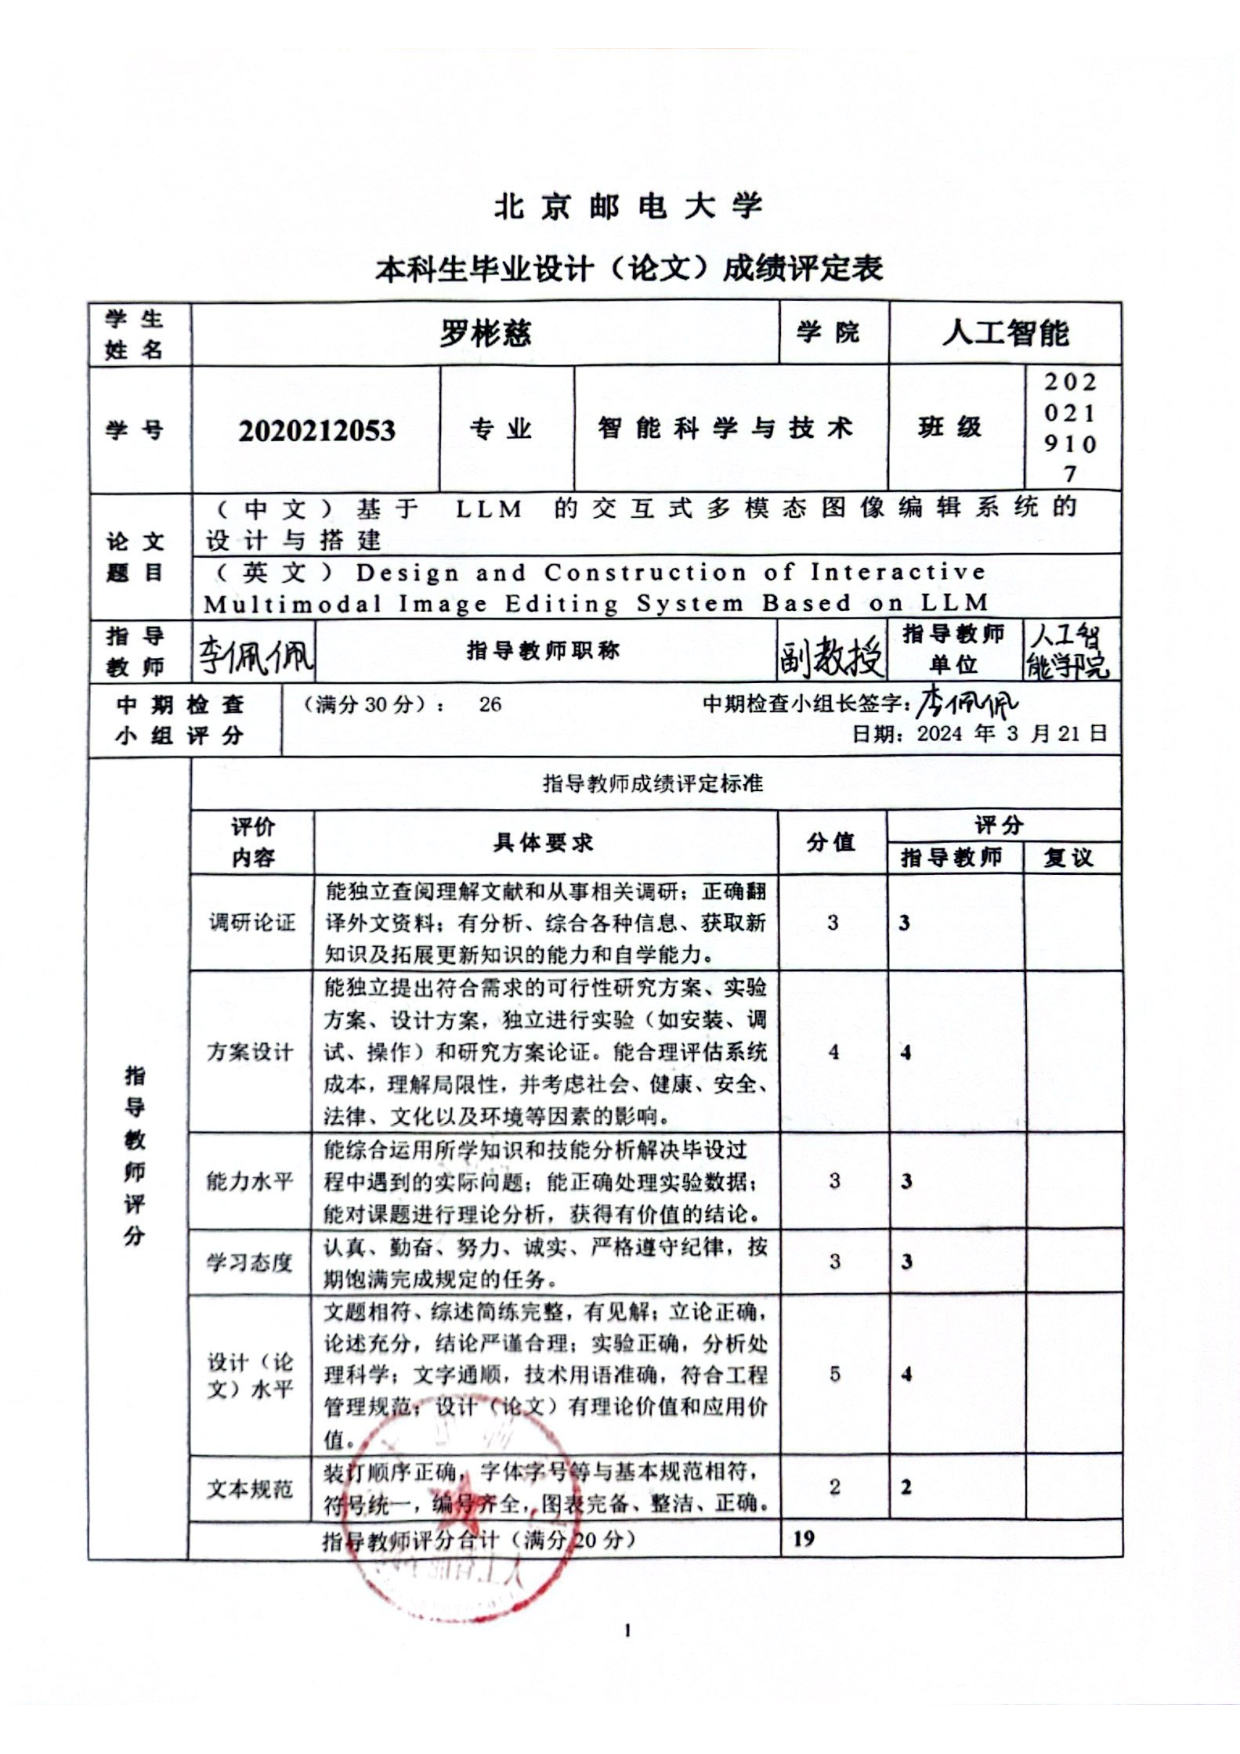
\includepdf[pages=-]{docs/ScoreTableScan.pdf}  



%%%%%%%%%%%%%%%%%%%%%%%%%%%%%%%%%%%%%%%%%%%%%%%%%%%%%%%%%%%%%%%%%%%%
%                                                                  %
%   Copyright (c) 2010 - 2011 Caspar Zhang <casparant@gmail.com>   %
%                                                                  %
%   This copyrighted material is made available to anyone wishing  %
%   to use, modify, copy, or redistribute it subject to the terms  %
%   and conditions of the GNU General Public License version 2.    %
%                                                                  %
%   This program is distributed in the hope that it will be        %
%   useful, but WITHOUT ANY WARRANTY; without even the implied     %
%   warranty of MERCHANTABILITY or FITNESS FOR A PARTICULAR        %
%   PURPOSE. See the GNU General Public License for more details.  %
%                                                                  %
%   You should have received a copy of the GNU General Public      %
%   License along with this program; if not, write to the Free     %
%   Software Foundation, Inc., 51 Franklin Street, Fifth Floor,    %
%   Boston, MA 02110-1301, USA.                                    %
%                                                                  %
%%%%%%%%%%%%%%%%%%%%%%%%%%%%%%%%%%%%%%%%%%%%%%%%%%%%%%%%%%%%%%%%%%%%

% 你只需要修改下面几行就可以完成大部分内容的填写,
% 这要求你具有一定的LaTeX基础,但是如果你足够聪明,
% 不具有LaTeX基础也可以完成。

% 论文中文题目
\def\thesistitle{基于LLM的交互式多模态图像编辑系统的设计与搭建}

% 论文英文题目
%提示:英文摘要页的标题注意格式要求。
\def\thesistitleen{Design and Construction of Interactive Multimodal Image Editing System Based on LLM}

% Thank Words
\def\thankwords{

致谢的内容。
}
    % Main items 
%%%%%%%%%%%%%%%%%%%%%%%%%%%%%%%%%%%%%%%%%%%%%%%%%%%%%%%%%%%%%%%%%%%%
%                                                                  %
%   Copyright (c) 2010 - 2011 Caspar Zhang <casparant@gmail.com>   %
%                                                                  %
%   This copyrighted material is made available to anyone wishing  %
%   to use, modify, copy, or redistribute it subject to the terms  %
%   and conditions of the GNU General Public License version 2.    %
%                                                                  %
%   This program is distributed in the hope that it will be        %
%   useful, but WITHOUT ANY WARRANTY; without even the implied     %
%   warranty of MERCHANTABILITY or FITNESS FOR A PARTICULAR        %
%   PURPOSE. See the GNU General Public License for more details.  %
%                                                                  %
%   You should have received a copy of the GNU General Public      %
%   License along with this program; if not, write to the Free     %
%   Software Foundation, Inc., 51 Franklin Street, Fifth Floor,    %
%   Boston, MA 02110-1301, USA.                                    %
%                                                                  %
%%%%%%%%%%%%%%%%%%%%%%%%%%%%%%%%%%%%%%%%%%%%%%%%%%%%%%%%%%%%%%%%%%%%

% 你只需要修改下面内容就可以完成中英文摘要,
% 这要求你具有一定的LaTeX基础,但是还是那句话,
% 如果你足够聪明,不具有LaTeX基础也可以完成。

% 中文摘要
\def\abstractzh{
%从这里开始写你的摘要,分段需要空一行。
随着深度学习技术在图像处理领域和文本生成领域的迅速发展,多模态交互系统的构建已成为研究的热点。本文介绍了一个基于最新图像生成模型和大语言模型的交互式多模态图像编辑系统的设计与搭建。系统利用了Stable Diffusion、DALL-E等图像生成模型和ChatGPT系列、ChatGLM2-6B等大语言模型,通过图形用户界面(GUI)、中间件(middleware)进行图像生成模型和大语言模型的整合,实现了一个既直观又高效的基于文本交互的多模态图像编辑系统。用户可以通过简单的文本指令控制图像编辑过程,系统能够自动解析这些指令并修改图像。本项目评估了系统在实际应用中的表现,结果显示该系统能够有效地提高图像编辑效率和用户交互体验。
%摘要结束
}

% 中文关键字 
% TODO: 改成可变长度的
\def\abszhkeyone{图像编辑}
\def\abszhkeytwo{大语言模型}
\def\abszhkeythree{多模态}
% \def\abszhkeyfour{模板}
% \def\abszhkeyfive{示例}

% ABSTRACT
\def\abstracten{
%Your abstract here, to make a new paragraph, give an extra blank line please.
With the rapid development of deep learning technology in the fields of image processing and text generation, the construction of multimodal interaction systems has become a hot topic of research. This paper introduces the design and construction of an interactive multimodal image editing system based on the latest image generation models and large language models. Utilizing image generation models such as Stable Diffusion and DALL-E, and large language models such as the ChatGPT series and ChatGLM2-6B, the system integrates these models through a graphical user interface (GUI) and middleware. This setup achieves an intuitive and efficient text-based multimodal image editing system. Users can control the image editing process through simple text commands, and the system can automatically parse these instructions and modify images. The project evaluated the system's performance in practical applications, and the results show that the system effectively improves image editing efficiency and user interaction experience.
%Abstract done
}

% Key Words 
% TODO: 改成可变长度的
\def\absenkeyone{Image Editing}
\def\absenkeytwo{Large Language Models}
\def\absenkeythree{Multimodal}
% \def\absenkeyfour{template}
% \def\absenkeyfive{example}


  % Abstract

\fancypagestyle{plain}{\pagestyle{frontmatter}}
\frontmatter
\tableofcontents % Content

% 正文
\newpage\mainmatter
\fancypagestyle{plain}{\pagestyle{mainmatter}}

%\let\cleardoublepagebak=\cleardoublepage
%\let\cleardoublepage\relax % Make new chapter stay on old page

%%%%%%%%%%%%%%%%%%%%%%%%%%%%% Main Area %%%%%%%%%%%%%%%%%%%%%%%%%%%%

\chapter{绪论} % 2085 + 66 + 25 = 2176
\section{项目背景与意义}
\subsection{项目背景}
随着技术的迅速发展,图像生成编辑在媒体娱乐、数字营销等领域等多个行业中发挥越来越重要的作用,
然而传统的图像编辑技术在交互性和生成图像质量上仍面临许多挑战。
传统图像编辑工具往往依赖于专业的技术知识和复杂的操作界面,交互性通常较差,不能很好地根据用户的具体需求进行灵活调整和响应,对于普通用户来说门槛较高,
用户需要花费大量时间学习如何使用这些工具,限制了工具的普及性和易用性。

为了改善图像编辑的交互性和灵活性,人们正在利用深度学习技术来改善图像编辑系统。
目前的研究显示扩散模型已经在图像生成领域具有巨大的潜力,其能够学习大量图像数据,自动提取复杂的特征,并生成高质量的图像。若将其运用于图像编辑,或许可以改善图像编辑的质量。
对于交互性,若将最新的GPT4Turbo等性能优异的大语言模型融入到图像编辑系统中,或许可以进一步提升系统的交互性,实现更加自然和直观的交互。

通过将图像生成模型与大语言模型结合,可以创建一个更加灵活且易用性强的图像编辑系统,
该系统不仅能够提供更加直观的编辑界面,降低用户的操作难度,还能根据用户的描述自动生成或修改图像,
极大地提升生成图像的质量和编辑效率。用户可以通过简单的语言指令,如“增加图片亮度”或“改变背景为海滩”,
直接与编辑系统交互,系统能够理解这些指令并即时作出响应。

通过整合深度学习和语言模型技术,我们有望构建出一个全新的交互式图像编辑系统,其不仅能够提供更高质量的图像编辑结果,更能够提供给用户更加自然的交互方式,为该领域的专业人士和普通用户都带好的图像编辑体验。
\subsection{项目意义}
通过融合先进的图像生成技术与大语言模型,本项目希望能搭建一个基于LLM的交互式图像编辑系统,提供更为易用、精准且高效的图像编辑工具,提升媒体娱乐、数字营销以及智能医疗等多个行业的图像处理能力。
通过实现更加智能化和用户友好型的编辑系统,为广大用户带来前所未有的图像编辑体验。这样的研究与开发,为图像编辑技术的未来提供了一种可能性和一条新的探索和实践路径。
\section{国内外研究现状}
Multimodal image synthesis and editing: A survey\cite{zhan2022multimodal}这篇论文对多模态图像合成和编辑的进展进行了综述,讨论如何有效地结合多种模态信息来创造和编辑图像。该论文提出了一种分类体系,根据数据模态和模型架构进行分类,并详细介绍了多模态图像合成和编辑的各种方法。该论文还讨论了基准数据集、评价指标以及当前研究中的挑战,并提出了未来的研究方向,强调在图像合成和编辑任务中引入跨模态指导的重要性和潜力。
\subsection{图像编辑}
ImageBART\cite{esser2021imagebart}是一种基于自回归变换的图像生成和编辑模型,灵感来源于自然语言处理中的 BART(Bidirectional and Auto-Regressive Transformers)\cite{lewis2019bart},其结合了自回归和编码-解码架构,用于高效地生成和编辑图像。
EditGAN\cite{ling2021editgan}提出了一种高精度的语义图像编辑方法,允许用户通过修改图像的详细部分分割掩模来编辑图像,其基于生成对抗网络(GAN)构建,只需要少量标记样本即可进行训练,实现了高效的编辑。
Generating images from captions with attention\cite{mansimov2015generating}介绍了一个能从自然语言描述中生成图像的模型,这个模型在关注描述中的相关词汇的同时利用深度循环注意力编写器(DRAW)迭代地在画布上绘制图像。
Object-based image editing\cite{barrett2002object}介绍了基于对象的图像编辑技术,允许用户直接在对象层面而不是像素层面进行编辑。
Faceshop: Deep sketch-based face image editing\cite{portenier2018faceshop}提供了一种利用深度学习来进行面部图像编辑的方法。
Image-based modeling and photo editing\cite{oh2001image}探讨了基于图像的建模与照片编辑技术,特别强调了分层编辑和实体分离技术的应用。
Invertible conditional gans for image editing\cite{perarnau2016invertible}探索了可逆Conditional GANs在图像编辑中的应用,这种模型结合了编码器和cGAN,可对真实图像进行精确修改。
In-domain gan inversion for real image editing\cite{zhu2020domain}研究了在领域GAN反转技术在真实图像编辑中的应用,通过GAN学习特定图像域的编辑操作。
Poisson image editing\cite{di2016poisson}探讨了泊松图像编辑技术,该技术能够无缝地将图像区域融合和编辑,并提供高质量的编辑效果。
Image editing in the contour domain\cite{elder1998image}提出了一种在轮廓域进行图像编辑的方法,这种方法直接在轮廓层面而不是像素层面进行操作。
Diffusion maps for edge-aware image editing\cite{farbman2010diffusion}使用扩散映射技术进行边缘感知图像编辑以在保持边缘清晰的同时平滑颜色和纹理。
\subsection{大语言模型微调}
Parameter-efficient fine-tuning of large-scale pre-trained language models\cite{ding2023parameter}介绍了Delta-tuning技术,它在不改变预训练大模型(PLMs)架构的基础上,通过微调少量参数来适应新任务。其主要包括以下方法:增加式、指定式和重新参数化方法,以及在变换器层添加适配器模块的实际应用,这些方法比全参数微调更节省计算资源,提高了模型的适应性和效率。
How fine can fine-tuning be? learning efficient language models\cite{radiya2020fine}分析了微调过程的效率,对在保持性能的同时减少计算成本的方法进行探索。
\# InsTag: Instruction Tagging for Analyzing Supervised Fine-tuning of Large Language Models\cite{lu2023instag}使用指令标签分析监督式微调过程,以提高大型语言模型在特定任务上的性能。
Scaling federated learning for fine-tuning of large language models\cite{hilmkil2021scaling}应用联邦学习方法来微调大型语言模型,以提高模型在多个数据源上的通用性和隐私保护。
Longlora: Efficient fine-tuning of long-context large language models\cite{chen2023longlora}针对长上下文的大型语言模型进行高效微调,以提升模型对长距离依赖信息的处理能力。
Fine-tuning pre-trained language models effectively by optimizing subnetworks adaptively\cite{zhang2022fine}通过自适应优化子网络来有效微调预训练语言模型,以提高模型的灵活性和适应新任务的能力。
Llm-adapters: An adapter family for parameter-efficient fine-tuning of large language models\cite{hu2023llm}提出一种用于大型语言模型参数高效微调的适配器家族,以减少模型调整过程中的资源消耗。
Language models are few-shot learners\cite{brown2020language}探讨语言模型在小样本学习中的表现,并分析其微调和适应新任务的能力。
Fine-tuning language models with just forward passes\cite{malladi2024fine}提出一种仅通过前向传播进行微调的新方法,以简化语言模型的调整过程。
\subsection{多模态图像编辑方法}
PixelTone: A Multimodal Interface for Image Editing\cite{laput2013pixeltone}介绍了一种结合语音和直接操作的多模态照片编辑界面,旨在简化移动设备上的图像编辑任务,通过自然语言和草图来定位图像中的具体更改区域。研究还开发了一个定制的自然语言解释器,将用户的语言指令映射到具体的图像处理操作上。通过用户研究,验证了接口的有效性,展示了其在简化编辑流程和提高用户互动体验方面的潜力。
DiffusionCLIP\cite{kim2022diffusionclip}是一种结合了扩散模型和CLIP\cite{radford2021learning}模型的新型图像编辑方法。这种方法利用了扩散模型的生成能力和CLIP的语义理解能力,以实现通过文本描述来精确控制图像的内容和属性的编辑。
Language-based image editing with recurrent attentive models\cite{chen2018language}提出一种基于语言的图像编辑方法,通过递归注意模型允许用户用自然语言描述来指导图像编辑过程。
Imagic: Text-based real image editing with diffusion models\cite{kawar2023imagic}利用扩散模型和文本描述来进行真实图像的编辑,并允许细粒度控制和高度个性化的编辑。
Sequential attention GAN for interactive image editing\cite{cheng2020sequential}介绍了一个用于交互式图像编辑的顺序注意力GAN模型,允许用户通过多轮对话逐步指导图像编辑。
Towards automatic image editing: Learning to see another you\cite{ghodrati2015towards}研究了自动图像编辑的可能性,通过机器学习方法让系统能够根据用户的需求生成或修改图像。
Instructpix2pix: Learning to follow image editing instructions\cite{brooks2023instructpix2pix}使用pix2pix模型学习遵循图像编辑指令,使得模型能够根据文字描述自动进行图像编辑。
Blended diffusion for text-driven editing of natural images\cite{avrahami2022blended}使用自然语言界面和数据驱动的图像生成技术进行文本驱动的图像编辑。
Tigan: Text-based interactive image generation and manipulation\cite{zhou2022tigan}提出了一种基于文本的交互式图像生成和操作框架。
Shape-aware text-driven layered video editing\cite{lee2023shape}对基于形状感知的文本驱动分层视频编辑方法进行探索。
Prompt tuning inversion for text-driven image editing using diffusion models\cite{dong2023prompt}使用扩散模型,为基于文本的图像编辑提供一种新的反演方法。
Lightweight text-driven image editing with disentangled content and attributes\cite{li2023lightweight}提供了通过解耦内容和属性以进行轻量级的基于文本驱动的图像编辑的方法。

\section{项目内容及创新点}
\subsection{项目内容}
\buptfigure[width=0.5\textwidth]{pictures/arch.png}{项目整体结构}{arch_TMP}

% 该项目主要实现了GUI、Middleware,并对Stable Diffusion和ChatGLM2-6B进行修改与适配。
% 各个模块之间的关系如 图1-1 所示。

% 通过在基于Stable Diffusion的开源项目stable-diffusion-webui上进行扩展,
% 本项目实现了通过API调用多种Stable Diffusion模型对图像进行修改的功能。

% 通过对ChatGLM2-6B进行微调,本项目实现了通过API调用针对本任务微调过的ChatGLM2-6B模型。

% 通过调用OpenAI的API,本项目实现了多个功能:通过GPT4V生成图像修改的建议、
% 通过GPT3.5Turbo辅助生成微调大语言模型的数据集和图像修改的指令、
% 通过DALL-E2实现在Stable Diffusion不可用时作为替代模型对图像进行修改。

% GUI主要通过python语言实现,其构建了一个直观、易于使用的用户交互界面。
% 在消耗大量计算资源的任务上,GUI会通过API对Middleware发出请求,
% 减少了用户侧对计算资源的依赖,降低了用户的使用门槛。

% Middleware使用golang语言搭建了一个后端服务,其接入了Stable Diffusion、ChatGLM2-6B、OpenAI的API,并将这些API进行整合后向GUI提供API。Middleware的建立实现了一对多服务的能力,提高了GUI调用多方API的便利性,同时通过统一配置提高了系统的可维护性。

该项目是一个多模态交互式图像编辑系统,它主要实现了GUI、Middleware、以及对Stable Diffusion和ChatGLM2-6B模型的修改与适配。在整体结构上,GUI、Middleware、以及模型修改之间的相互关系和数据流向见 图1-1。

项目基于Stable Diffusion的开源项目stable-diffusion-webui进行了扩展,增强了其功能。系统可以调用不同的Stable Diffusion模型并结合多个扩展后的功能来对图像进行精细的修改和调整。这一功能的实现大大增强了系统对图像处理的灵活性和多样性。

项目还包括了对ChatGLM2-6B模型的微调。通过利用专门为本项目的需求生成的微调数据集进行微调,进一步提升了语言模型处理特定任务的能力和准确性,且能够利用API调用这些经过微调的ChatGLM2-6B模型。

通过调用OpenAI的API,本项目实现了多项功能:利用GPT4V生成关于图像修改的建议,使用GPT3.5Turbo来辅助生成用于微调大语言模型的数据集以及图像修改指令,以及在Stable Diffusion模型不可用时,使用DALL-E2作为替代模型来进行图像修改。这些功能为基于LLM的交互式图像编辑系统提供了强大的工具。

在GUI方面,本系统主要通过Python语言实现,构建了一个直观且用户友好的交互界面。该界面简洁易用,通过API调用向Middleware发出请求,有效减轻了用户在执行计算密集型任务时对硬件资源的需求,从而降低了用户侧的使用门槛。

Middleware部分使用Golang语言构建了一个后端服务。这个服务不仅接入了Stable Diffusion、ChatGLM2-6B、OpenAI的API,还将这些API进行了有效的整合,向GUI提供了一致风格的API接口。这种设计不仅提升了GUI调用多方API的便利性,也通过统一的配置和管理,极大地增强了系统的可维护性和稳定性。

通过整合深度学习和大语言模型技术,本项目不仅能够提供更高质量的图像编辑结果,还能为用户提供更加自然的交互方式,极大地提升了图像编辑的效率和体验。此外,系统设计中还考虑了扩展性和未来技术的整合,预留了接口以适应未来可能的升级,以适应快速发展的技术需求。

\subsection{项目创新点}
本项目的方案设计充分考虑了技术实现的可行性与用户操作的便捷性,力求在满足复杂功能需求的同时,保证系统的易用性和稳定性。
本项目将复杂的模型调用参数抽象为用户可理解的模版与设置,建立了一个基于JSON的指令机制打通了大语言模型与图像生成模型,同时对多种主流大语言模型和图像编辑模型进行适配预留有接口,可随着大语言模型和图像生成模型技术的发展快速迭代。
通过系统化的设计和技术的整合,本项目实现了一个高效且用户友好的多模态交互式图像编辑系统。

\section{论文结构}
本论文共分为七个章节,每个章节的具体内容如下:

第一章,绪论。本章主要论述了基于LLM的交互式多模态图像编辑系统的项目背景与意义,总结了相关的国内外研究现状,简述了项目内容并列举了项目创新点。

第二章,相关技术研究。本章主要介绍了本项目所使用到的相关技术,包括扩散模型、基于扩散模型的可控图像生成、大语言模型、系统开发工具。

第三章,基于LLM的交互式多模态图像编辑系统的需求分析。本章主要对系统业务与用户角色进行分析,结合本项目所使用技术的特点和传统图像编辑系统的痛点,分析了系统功能需求。

第四章,基于LLM的交互式多模态图像编辑系统的设计与实现。本章主要论述系统的设计与实现方式,包括GUI与Middleware的构建、多模态的实现、LLM的微调、StableDiffusion及扩展的使用。

第五章,系统实现效果与使用。本章主要展示了系统实现效果,并对系统使用方法进行说明。

第六章,项目管理与维护。本章主要论述了项目所使用的管理与维护方法,包括代码管理、自动化测试、持续集成与持续部署。

第七章,总结及未来展望。本章对全文和开发工作进行总结与归纳,并提出基于LLM的交互式多模态图像编辑系统的未来展望。

\chapter{相关技术研究}
\section{扩散模型}
扩散模型是近年来发展起来的一种新型生成模型,与传统的生成对抗网络(GANs)和变分自编码器(VAEs)相比,扩散模型在生成图像的质量和多样性方面展现出了卓越的性能,其基本原理是模拟从高质量数据分布到高熵噪声分布的逐步转变过程,然后再逆向这一过程以生成新的数据。
扩散模型的关键优势在于其生成的图像质量较高且自然,而且在训练过程中相对稳定,不易出现生成对抗网络中常见的模式崩溃问题,
其基本原理如下:

前向过程(Forward Process)也称为扩散过程逐步将原始数据 \( x_0 \) 加入高斯噪声,最终转化为纯噪声 \( x_t \)。此过程可以表示为算法1:
\begin{algorithm}
    \floatname{algorithm}{算法}
    \caption{扩散模型的前向过程}
    \begin{algorithmic}[1]
    \State 初始化 $x_0 \sim q(x_0)$
    \For{$t = 1$ 到 $T$}
        \State $x_t \sim q(x_t|x_{t-1}) = \mathcal{N}(x_t; \sqrt{1-\beta_t}x_{t-1}, \beta_t \mathbf{I})$
    \EndFor
    \end{algorithmic}
\end{algorithm}

反向过程(Reverse Process)是前向过程的逆过程,其能通过通过训练的参数化模型 \( \epsilon_\theta(x_t, t) \) 从纯噪声状态 \( x_t \) 逐步重构出原始数据 \( x_0 \)。此过程可以表示为算法2:
\begin{algorithm}
    \floatname{algorithm}{算法}
    \caption{扩散模型的反向过程}
    \begin{algorithmic}[1]
    \State 初始化 $x_T \sim \mathcal{N}(0, \mathbf{I})$
    \For{$t = T$ 到 $1$}
        \State 如果 $t > 1$,则采样 $z \sim \mathcal{N}(0, \mathbf{I})$,否则 $z = 0$
        \State $x_{t-1} = \frac{1}{\sqrt{\alpha_t}}\left(x_t - \frac{\beta_t}{\sqrt{1-\bar{\alpha}_t}}\epsilon_\theta(x_t, t)\right) + \sigma_t z$
    \EndFor
    \State \Return $x_0$
    \end{algorithmic}
\end{algorithm}


扩散模型的优化最小化真实噪声和模型估计噪声之间的差异,其过程可以表示为算法3:
\begin{algorithm}
    \floatname{algorithm}{算法}
    \caption{扩散模型的优化过程}
    \begin{algorithmic}[1]
    \Repeat
        \State 采样 $x_0 \sim q(x_0)$,$t \sim \text{Uniform}\{1, \dots, T\}$,$\epsilon \sim \mathcal{N}(0, \mathbf{I})$
        \State $\tilde{x}_t = \sqrt{\bar{\alpha}_t}x_0 + \sqrt{1-\bar{\alpha}_t}\epsilon$
        \State 对 $\nabla_\theta \|\epsilon - \epsilon_\theta(\tilde{x}_t, t)\|^2$ 进行梯度下降
    \Until{收敛}
    \end{algorithmic}
\end{algorithm}

Stable Diffusion\cite{rombach2022high} 是一种基于扩散模型的深度学习图像生成模型,它能够根据文本描述生成高质量的图像。
该模型采用了条件生成技术,允许用户通过文本指令来引导噪声逆向还原从而生成高质量的图片,在艺术创作、媒体娱乐、广告和数字营销等多个领域具有广泛的应用。


由于本项目对于图像生成模型的要求较高且需求复杂,为了便于结合Stable Diffusion模型和其他前沿研究成果及开源社区项目,本项目在构建Stable Diffusion模块时
以开源项目stable-diffusion-webui\footnote{https://github.com/AUTOMATIC1111/stable-diffusion-webui}为基础,
结合sd-webui-controlnet和sd-webui-roop等扩展,通过 API 为Middleware提供服务。当Stable Diffusion模型不可用时,系统则会调用OpenAI的DALL-E 2模型。DALL-E 2 是一个先进的图像生成模型,可以根据用户提供的文本描述生成详细、高质量的图像,其核心优势在于其创造力和多样性,能够在遵循描述的同时,创造出独特和富有创意的视觉内容。

\section{基于扩散模型的可控图像生成}
ControlNet\cite{zhang2023adding}是一种新的神经网络架构,用于在大型预训练的文本到图像扩散模型中添加空间条件控制。ControlNet的核心是利用预训练模型的深层和健壮的编码层作为强大的支撑,学习多种条件控制。该网络通过零初始化的卷积层(zero convolutions)连接,这些层从零开始逐步增长参数,确保训练初期不会引入有害的噪声。
通过使用ControlNet,用户可以更精细地控制图像生成过程,使生成的图像更贴近用户的具体需求,尤其是在空间布局和细节表达上。这种方法能够有效地减少试错循环,提高图像生成的效率和质量。其与Stable Diffusion结合的方式如图2-1所示(图片摘自论文Adding Conditional Control to Text-to-Image Diffusion Models\cite{zhang2023adding})。
\buptfigure[width=0.5\textwidth]{pictures/SDCN.png}{ControlNet与Stable Diffusion结合}{SDCN_TMP}




\section{大语言模型}
近些年大语言模型发展异常迅猛,其通过学习大量文本数据,能够出色地完成生成文本、回答问题、翻译语言等任务。随着算力的提升和语料的增加,大语言模型已经取得了显著的进步,并在多个应用场景中展现出了强大的能力。
目前大语言模型主要使用Transformers\cite{vaswani2017attention}架构,其能够有效处理长距离依赖问题。GPT(Generative Pre-trained Transformer)、BERT(Bidirectional Encoder Representations from Transformers)等主流大语言模型,通过大规模的语料进行预训练,对语言的深层次结构和语义的理解能力有了显著的提升,在应用方面展现出广泛的适用性。
在大语言模型中,最著名的便是OpenAI的GPT系列:
GPT-3.5 Turbo 是 OpenAI 开发的一款先进的自然语言处理模型,属于 GPT-3 系列的增强版本,在处理大量文本和生成文本方面表现出色;
GPT-4\cite{achiam2023gpt} 是 GPT-3 的后续版本,代表了目前最新一代的大语言模型技术,在模型结构和训练数据量上进行了大幅扩展,能够更准确地理解和生成复杂的文本,在理解上下文、维持一致性以及生成更自然的语言方面具有显著优势;
GPT-4V 是 GPT-4 的一个特殊版本,优化了图像标注、视觉问答等视觉任务,结合文本和视觉处理能力,能够更好地理解和生成与图像相关的文本内容。

ChatGLM2-6B是由清华大学开发的第二代开源双语(中英)对话模型,基于ChatGLM-6B进行迭代并提升了性能,
这款模型经过大规模预训练,实现了显著的性能提升,并在多个数据集上表现出色。
ChatGLM2-6B支持更长的对话上下文,并提高了推理速度和降低了显存占用,
使得即使在资源有限的环境下也能有效运行。本项目使用ChatGLM2-6B模型,结合开源项目LLaMA-Factory\footnote{https://github.com/hiyouga/LLaMA-Factory},
利用本项目提供的数据自动生成功能所生成的数据集,使用LoRA\cite{hu2021lora}方法对模型进行微调以在本项目所需的任务中获得更佳的表现。微调后的模型通过fastapi提供 API 服务。

LoRA通过在每个Transformer层中注入可训练的低秩矩阵对权重进行更新,而不是更新整个权重矩阵。这种方法不仅减少了模型的存储和计算成本,还保持了与完全微调相当的模型性能。其算法可概括为算法4。
\begin{algorithm}
    \begin{spacing}{1.3}
        \floatname{algorithm}{算法}
        \caption{LoRA: 低秩适应大型语言模型} 
        \label{alg:LoRA}
        \renewcommand{\algorithmicrequire}{\textbf{输入:}}
        \renewcommand{\algorithmicensure}{\textbf{输出:}} 
        \begin{algorithmic}[1] 
            \Require 预训练模型权重 $W_0 \in \mathbb{R}^{d \times k}$,输入 $x$, 低秩 $r$
            \Ensure 适应后的输出
            \State 初始化低秩矩阵 $A \in \mathbb{R}^{d \times r}$ 和 $B \in \mathbb{R}^{r \times k}$
            \State 设定更新权重 $\Delta W = BA$
            \State 冻结预训练权重 $W_0$
            \State \textbf{for} 每一层Transformer \textbf{do}
            \State \hspace{\algorithmicindent} 使用 $W = W_0 + \Delta W$ 进行前向传播
            \State \hspace{\algorithmicindent} 优化 $A$ 和 $B$ 来最小化损失函数
            \State \textbf{end for}
            \State 输出调整后的模型结果
        \end{algorithmic}
    \end{spacing}
\end{algorithm}

\section{系统开发工具}
Gradio 是一个开源的 Python 库,旨在简化为机器学习模型创建自定义用户界面的过程。
本项目使用Gradio框架构建了GUI组件以提供简单易用的交互界面。

beego是一个使用Go语言开发的开源Web框架,它支持快速开发各种应用程序,包括API、Web应用和后端服务。该框架设计灵感来源于Tornado、Sinatra和Flask,结合了Go的接口(interface)和结构体嵌入(struct embedding)等特性,提供了高效的性能和简便的操作​ 。
本项目使用beego框架构建了Middleware组件以提供多个API服务,以便GUI可以高效地使用各种模型和工具。

\section{本章小结}
在本章中,我们深入探讨了与多模态图像编辑系统相关的关键技术,首先详细介绍了扩散模型的工作原理及其在图像生成中的应用,接着讨论了大语言模型的相关信息与LoRA微调技术,最后概述了系统开发中使用的主要工具和方法。本章不仅为理解系统的技术基础提供了理论支撑,也为后续章节中系统设计和实现的详细讨论奠定了基础。






% Middleware是项目的核心组件,通过整合多个平台的API,为GUI提供统一的、简单易接入的API服务。其主要特点包括但不限于:
% 1. API整合:Middleware整合了多个平台的API,包括图像生成模型、语言模型等,使得GUI可以通过统一的接口调用不同功能模块;
% 2. 统一风格:Middleware设计了统一的API风格和路由规范,使得GUI可以轻松使用API服务,提高开发效率;
% 3. 简单易接入:Middleware提供了简单易用的API服务,GUI无需关注具体实现细节,只需按照简单的请求规范调用API即可;
% 4. 稳定性和可靠性:Middleware基于Golang语言实现,具有高效的并发处理能力和稳定的运行性能,保证了API服务的稳定性和可靠性;
% 5. 易于维护:Middleware采用了Beego框架,具有清晰的代码结构和模块化设计,易于维护和扩展,保证了项目的长期可持续发展。
% 其向GUI提供的主要API如 表2-2 所示:
% \begin{bupttable}{Middleware 主要API}{table_gui_modules}
%     \begin{tabular}{|l|l|l|}
%         \hline \textbf{API} & \textbf{路由} & \textbf{描述} \\
%         \hline PostSDTxt2Img & /v1/pics/txt2img & 通过Stable Diffusion模型生成图片  \\
%         \hline PostSDImg2Img & /v1/pics/img2img & 通过Stable Diffusion模型修改图片 \\
%         \hline PostDALLE2Edit & /v1/pics/openai/img2img & 通过DALL-E2模型修改图片  \\
% 		\hline GetLoras & /v1/pics/loras & 获取可用的LoRA模型列表  \\
% 		\hline PostHuggingFaceImgSegment & /v1/pics/huggingface/segment & 获取图像分割结果  \\
% 		\hline PostGPT3Dot5Turbo & /v1/chat/gpt3dot5turbo & 调用GPT3.5Turbo  \\
% 		\hline PostGPT4Turbo & /v1/chat/gpt4 & 调用GPT4Turbo  \\
% 		\hline PostChatGLM2\_6B & /v1/chat/glm2\_6b & 调用ChatGLM2-6B  \\
% 		\hline PostGPT4V & /v1/chat/gpt4v & 调用GPT4V  \\
%         \hline
%     \end{tabular}
% \end{bupttable}

\chapter{基于LLM的交互式多模态图像编辑系统的需求分析}
\section{系统业务与用户角色分析}
本项目的目标是构建一个基于LLM的交互式多模态图像编辑系统,结合大语言模型和图像生成技术,提供一个友好的图形用户界面,支持用户通过自然语言指令进行复杂的图像编辑操作,使非技术用户也能轻松使用复杂的图像编辑功能。
系统需能够理解和解析用户的自然语言指令,将其转换为具体的图像编辑任务,
并利用最新的图像生成模型如Stable Diffusion根据由用户的指令生成的相关参数修改图像。

本项目的目标用户群体包括设计师、营销专业人员、教育工作者和普通消费者。设计师可以利用系统快速实现创意构思,改善设计流程的效率。营销专业人员可以使用该系统快速调整广告图像,以适应不同的市场需求。教育工作者可以使用此系统来创建或修改教学资料中的图像,使教学内容更加生动有趣。普通消费者则可以利用系统提供的易于使用的平台,探索个人图像编辑和创意表达。

\section{系统功能需求分析}
项目旨在整合Stable Diffusion和大语言模型等最新的深度学习模型以实现通过自然语言指令实现高质量的图像编辑。图形用户界面(GUI)设计应简洁直观,包含预览功能,提升用户体验。中间件(Middleware)需高效处理GUI请求,并向模型API转发,确保系统稳定性和响应速度。系统应能高效处理复杂的图像编辑任务,并考虑多种使用场景和用户需求,以保证广泛应用和良好用户体验。

\section{本章小结}
本章主要对基于LLM的交互式多模态图像编辑系统进行了需求分析。项目旨在结合大语言模型和图像生成技术提供一个高效、直观的图像编辑系统,使用户能够轻松使用复杂的图像编辑功能。项目的目标用户群体包括设计师、营销专业人员、教育工作者和普通消费者,需支持用户通过自然语言指令利用图像生成模型进行高质量的图像编辑操作。系统需要整合多个深度学习模型、设计直观的GUI界面、实现高效处理请求的中间件,并考虑多种使用场景和用户需求,以提供良好的用户体验。


\chapter{基于LLM的交互式多模态图像编辑系统的设计与实现}
在本项目中,图形用户界面(GUI)作为用户与系统交互的前端界面扮演了至关重要的角色,不仅需要具备直观操作的特性,还应支持复杂的自定义图像处理功能,因此本项目将简洁且直观考虑为GUI设计中的重点,通过图形化元素如按钮、图标和菜单等,允许用户以简单的点击操作来进行交互。GUI还集成了一些预览功能,用户可以查看遮罩效果,有效提升用户体验和操作的精确性。

Middleware负责处理来自GUI的请求,在本系统中起到了桥梁的作用。Middleware采用了高效的Golang语言结合beego框架进行构建以保证系统的响应速度和稳定性,将来自GUI的请求进行处理并向对应的部署在云平台或OpenAI的模型调用API转发。它整合了包括Stable Diffusion、ChatGLM2-6B及OpenAI提供的API等多种服务,通过提供统一风格的API接口,极大地简化了GUI与模型之间的交互复杂度,不仅提高了开发效率,也便于系统的后期维护和升级。

图像编辑和文本交互方面所用到的图像生成模型和大语言模型是本项目的核心技术。项目中采用了最新的扩散模型技术——Stable Diffusion,其通过学习大量的图像数据,能够生成高质量的图像内容。项目还引入了大语言模型(如GPT系列和ChatGLM2-6B)来处理和理解用户的自然语言指令,实现更加智能的图像编辑功能。用户可以使用简单的语言描述如“将背景更换为海滩”来进行图像编辑,系统能够将用户输入自动解析为特定指令并进行相应的图像编辑。

通过整合GUI、Middleware、图像生成模型和大语言模型,本项目能够接受用户的文本输入并进行相应的复杂图像编辑。系统的设计考虑到了多种使用场景和用户的不同需求,确保了广泛的应用性和良好的用户体验。


\section{GUI的构建} % 1674+226 + 257 + 139 = 2296
图形用户界面是现代软件项目中不可或缺的组成部分,它极大地提升了应用程序的可访问性和用户体验。GUI通过可视化元素如按钮、图标和菜单等,允许用户以直观的方式与系统进行交互,简化了操作过程并降低了用户的使用门槛。
本项目所构建的GUI为用户提供了一个交互方式简单且功能强大的图形用户界面,通过图形化的方式展示信息和选择,使得用户能够通过简单的点击或触摸来执行命令或更改设置。
GUI虽然承担计算任务较少,但却是承载本项目结构与逻辑的关键部分。通过使用符合规则的指令作为中枢,
GUI打通了大语言模型和图像生成模型之间的壁垒,使基于LLM的创新交互式图像编辑系统成为可能。GUI的模块构成如 表4-1 :
\begin{bupttable}{GUI模块}{table_gui_modules}
    \begin{tabular}{|l|l|}
        \hline \textbf{模块} & \textbf{描述} \\
        \hline BaseImage & 接受上传的原始图片并预览  \\
        \hline EditedImage & 预览修改后的图片 \\
        \hline Operation Board & 执行指令  \\
		\hline Settings & 对系统进行设置  \\
		\hline Chat & 与大语言模型交互的聊天界面  \\
		\hline Edit Image & 对图像进行自定义遮罩和换脸等操作  \\
		\hline Auto & 执行自动化操作  \\
		\hline Manual & 系统使用说明  \\
        \hline
    \end{tabular}
\end{bupttable}

用户首先上传需要修改的图片,然后可在Chat模块中选择不同的大语言模型进行交互并得到相应的指令,
最后在Operation Board模块中选择指令执行或一键全部执行。如果对自动生成的遮罩不满意,
可在Edit Image中对遮罩进行修改。

在Auto模块中,用户可通过选择多张图片批量生成满足微调大语言模型微调所需的数据。
其会循环地从给定的图片集中随机选择图片继续分割,将分割后的结果和特定的prompt通过GPT3.5Turbo生成对应的修改建议,
再将分割的结果、生成的建议通过GPT3.5Turbo生成指令。

% 在本项目中,GUI作为关键组成部分,虽仅承担极少的计算任务,却在结构与逻辑上起着至关重要的作用。
% 它通过使用标准化的指令连接大语言模型和图像生成模型,实现了基于LLM的创新交互式图像编辑系统。
% 用户首先上传原始图片至BaseImage模块进行预览,之后可通过Chat模块与大语言模型进行交互,获取编辑指令。
% 用户可以在Operation Board模块中选择单独或批量执行这些指令。
% 若对自动生成的遮罩不满意,可在Edit Image模块中手动调整。
% 此外,Auto模块允许用户批量处理多张图片,自动生成数据以微调大语言模型。
% 该过程包括图片的自动分割、利用GPT3.5Turbo生成编辑建议及相应的执行指令。
% 这样的设计不仅提升了系统的效率,也优化了用户的交互体验。
\subsection{图像自动遮罩与优化}
由于本项目需要提供对图像进行部分修改的功能,所以需要在使用图像生成模型进行图像编辑时需要提供一个遮罩以明确需要修改的部分和不需要修改的部分。
为了自动生成符合要求的遮罩,本项目借助图像分割和大语言模型的辅助,可通过两种方式生成自动遮罩:基于关键词对自动生成遮罩和基于已给出的点自动填充生成遮罩。
两种方法都会首先使用图像分割模型对图像进行分割(如图4-1),然后根据给出的要求对相应的部分进行遮罩生成原始的遮罩。受制于图像分割模型在边缘上的表现并不理想,
需要对特定的分割部分进行处理以提高遮罩的质量,因此最后会通过本项目设计的优化算法生成最终的遮罩。
\begin{figure}[!htbp]
    \centering
    \subfloat[]{ %[]对齐方式,t为top,b为bottom,留空即可
	\label{Fig:SegmentOrigin1} % 子图1标签名
    	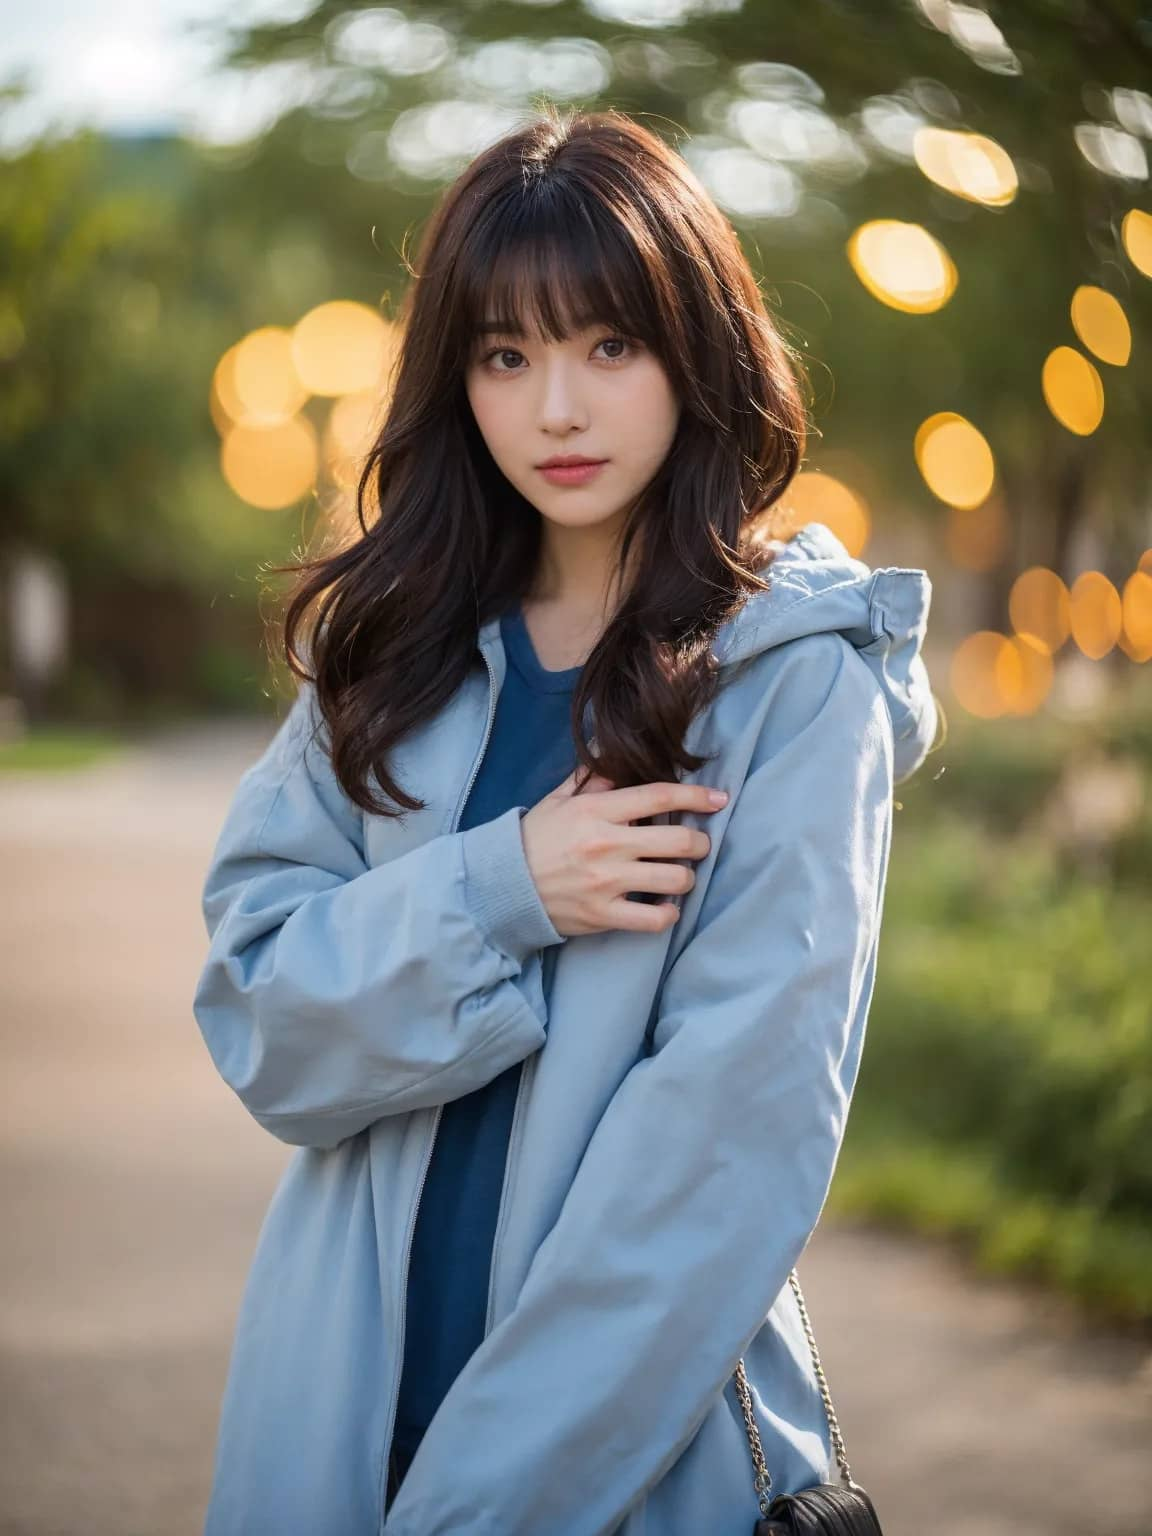
\includegraphics[width=0.24\textwidth]{pictures/example1_origin} %插入图片命令,格式为[配置]{图片路径}
    }
    \quad %空格
    \subfloat[]{
	\label{Fig:SegmentResult1} % 子图2标签名
    	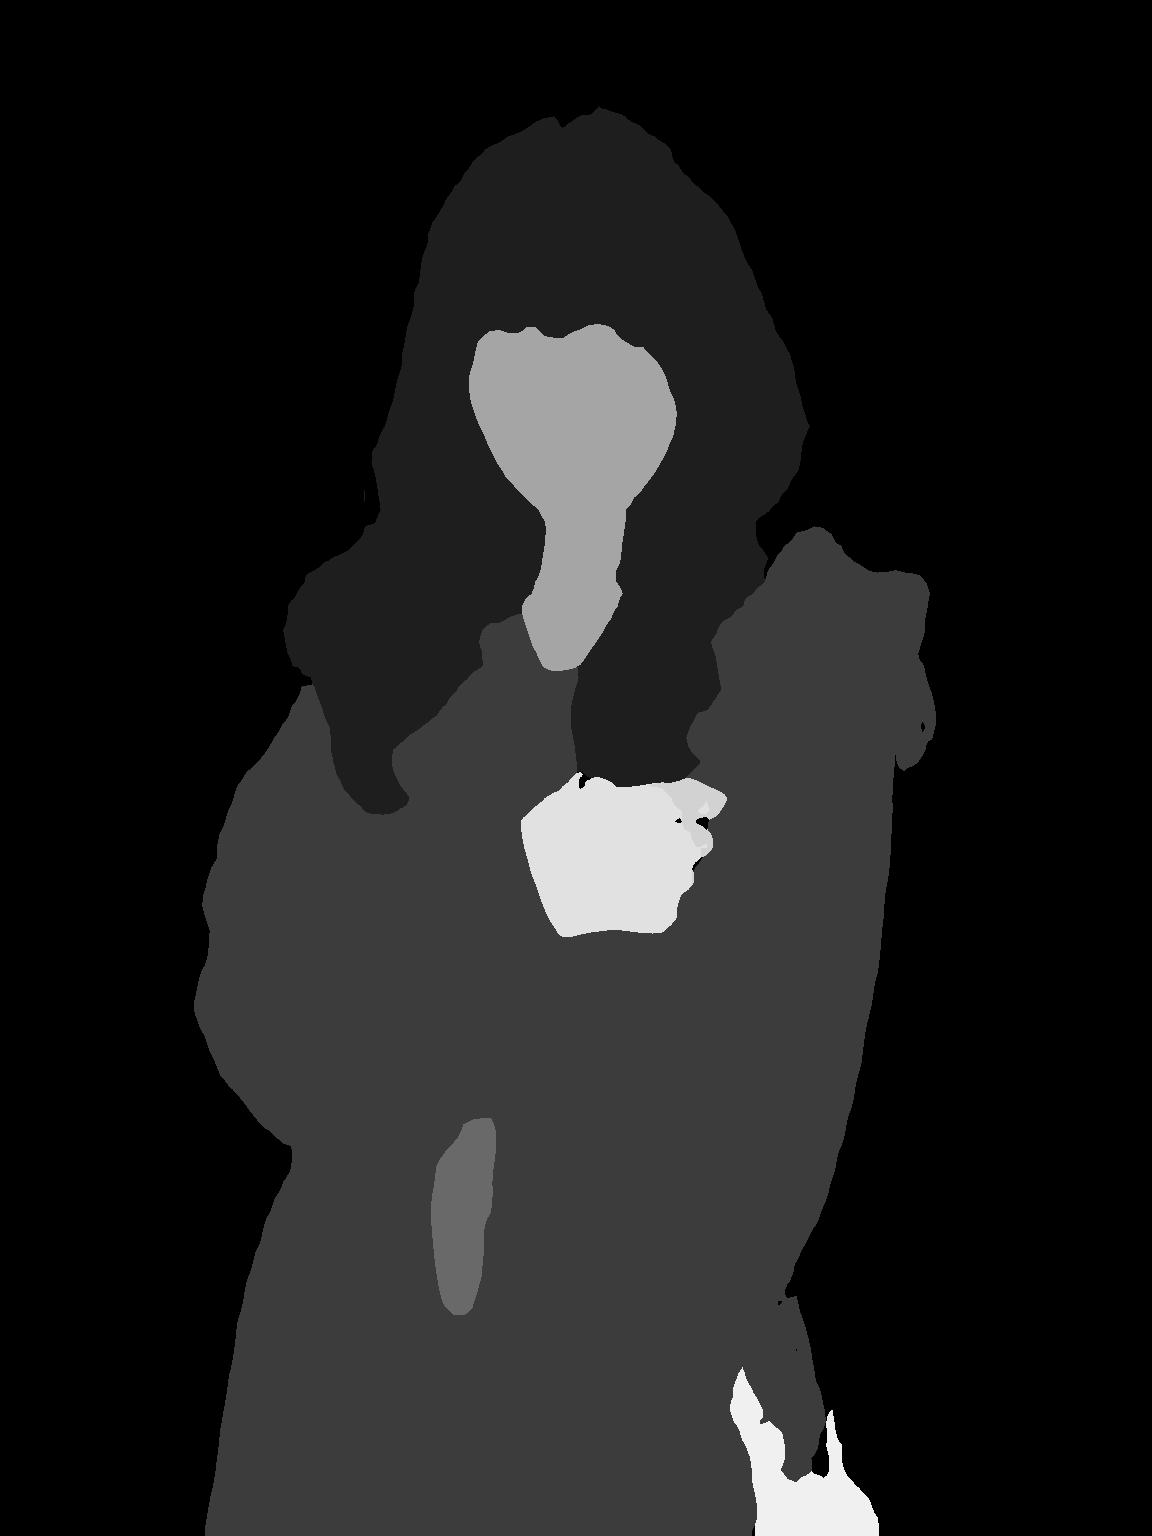
\includegraphics[width=0.24\textwidth]{pictures/example1_segment}
    }
    \caption{图像分割结果:\protect\subref{Fig:SegmentOrigin1}原始图像,\protect\subref{Fig:SegmentResult1}分割结果} %注意须使用\protect\subref{}进行标号引用
    \label{Fig:Segment} % 整个组图的标签名
\end{figure}

\subsubsection{图像自动遮罩}
基于关键词自动生成遮罩的方法会根据关键词和图像分割结果生成自动原始的遮罩,该功能会遍历每个给出的关键词,
若关键词与分割结果之一吻合,则会对相应的分割区域进行遮罩,生成原始的遮罩(如图4-2)。
\begin{figure}[!htbp]
    \centering
    \subfloat[]{ %[]对齐方式,t为top,b为bottom,留空即可
	\label{Fig:SegmentOrigin2} % 子图1标签名
    	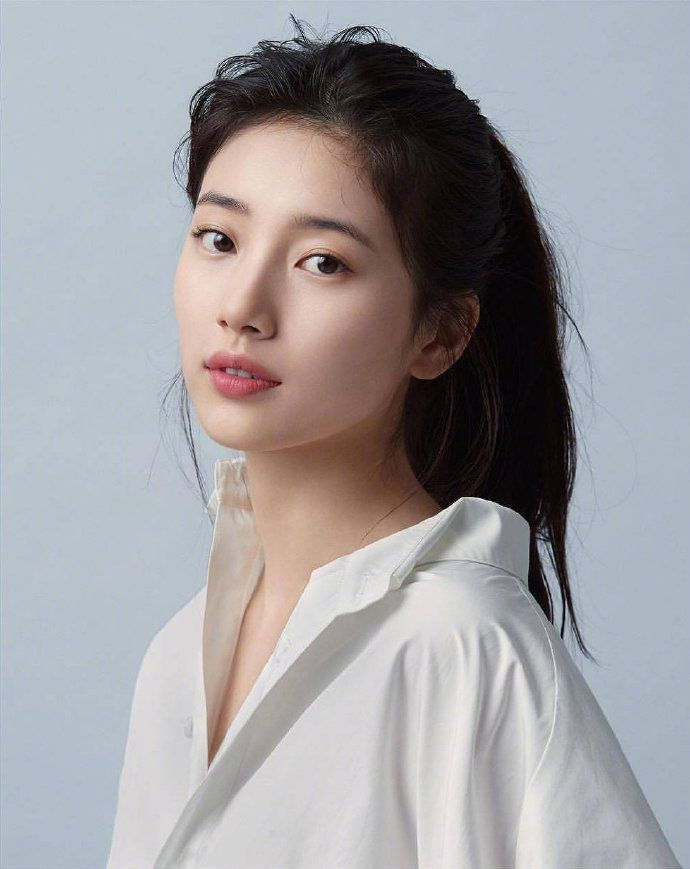
\includegraphics[width=0.24\textwidth]{pictures/example2_origin} %插入图片命令,格式为[配置]{图片路径}
    }
    \quad %空格
    \subfloat[]{
	\label{Fig:SegmentResult2} % 子图2标签名
    	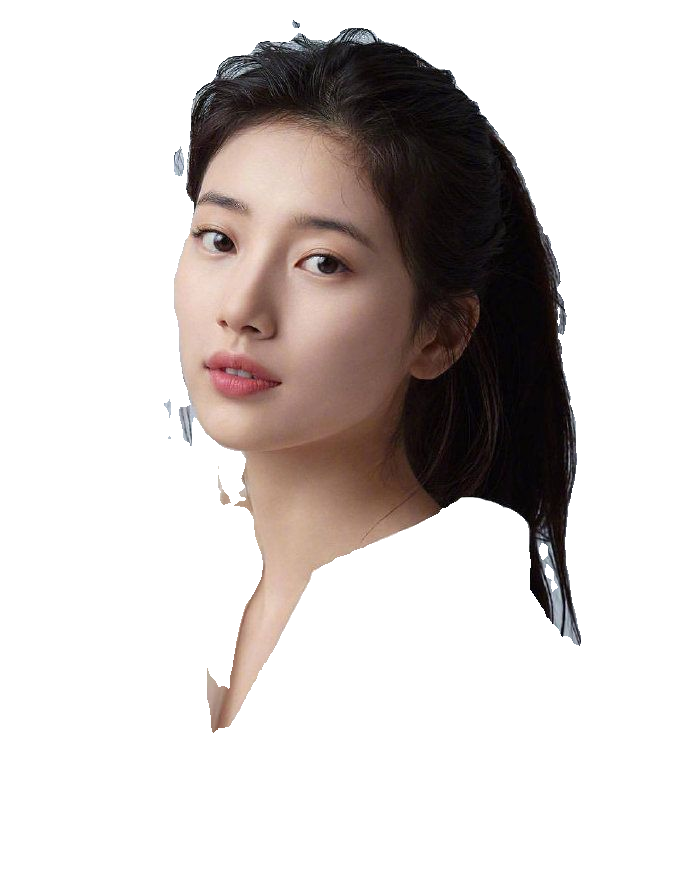
\includegraphics[width=0.24\textwidth]{pictures/example2_step1}
    }
    \caption{关键词自动生成遮罩结果:\protect\subref{Fig:SegmentOrigin2}原始图像,\protect\subref{Fig:SegmentResult2}kewords=['Background', 'Upper-clothes', 'Dress', 'Right-arm']得到的遮罩} %注意须使用\protect\subref{}进行标号引用
    \label{Fig:SegmentKeywords} % 整个组图的标签名
\end{figure}

基于已给出的点自动填充生成遮罩的方法会根据在图片中标记的点和图像分割结果生成自动原始的遮罩,该功能会遍历每个给出的点,
将该点所在的部分全部进行遮罩,最后生成原始的遮罩(如图4-3)。
\begin{figure}[!htbp]
    \centering
    \subfloat[]{
	\label{Fig:SegmentPoints} 
    	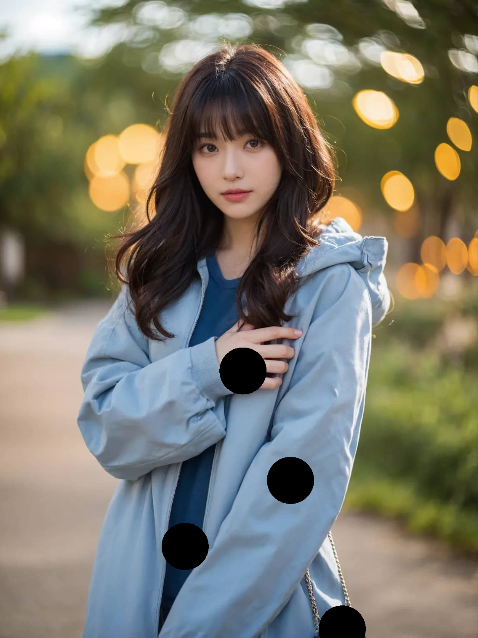
\includegraphics[width=0.24\textwidth]{pictures/example1_points}
    }
    \quad %空格
    \subfloat[]{
	\label{Fig:SegmentStep1} 
    	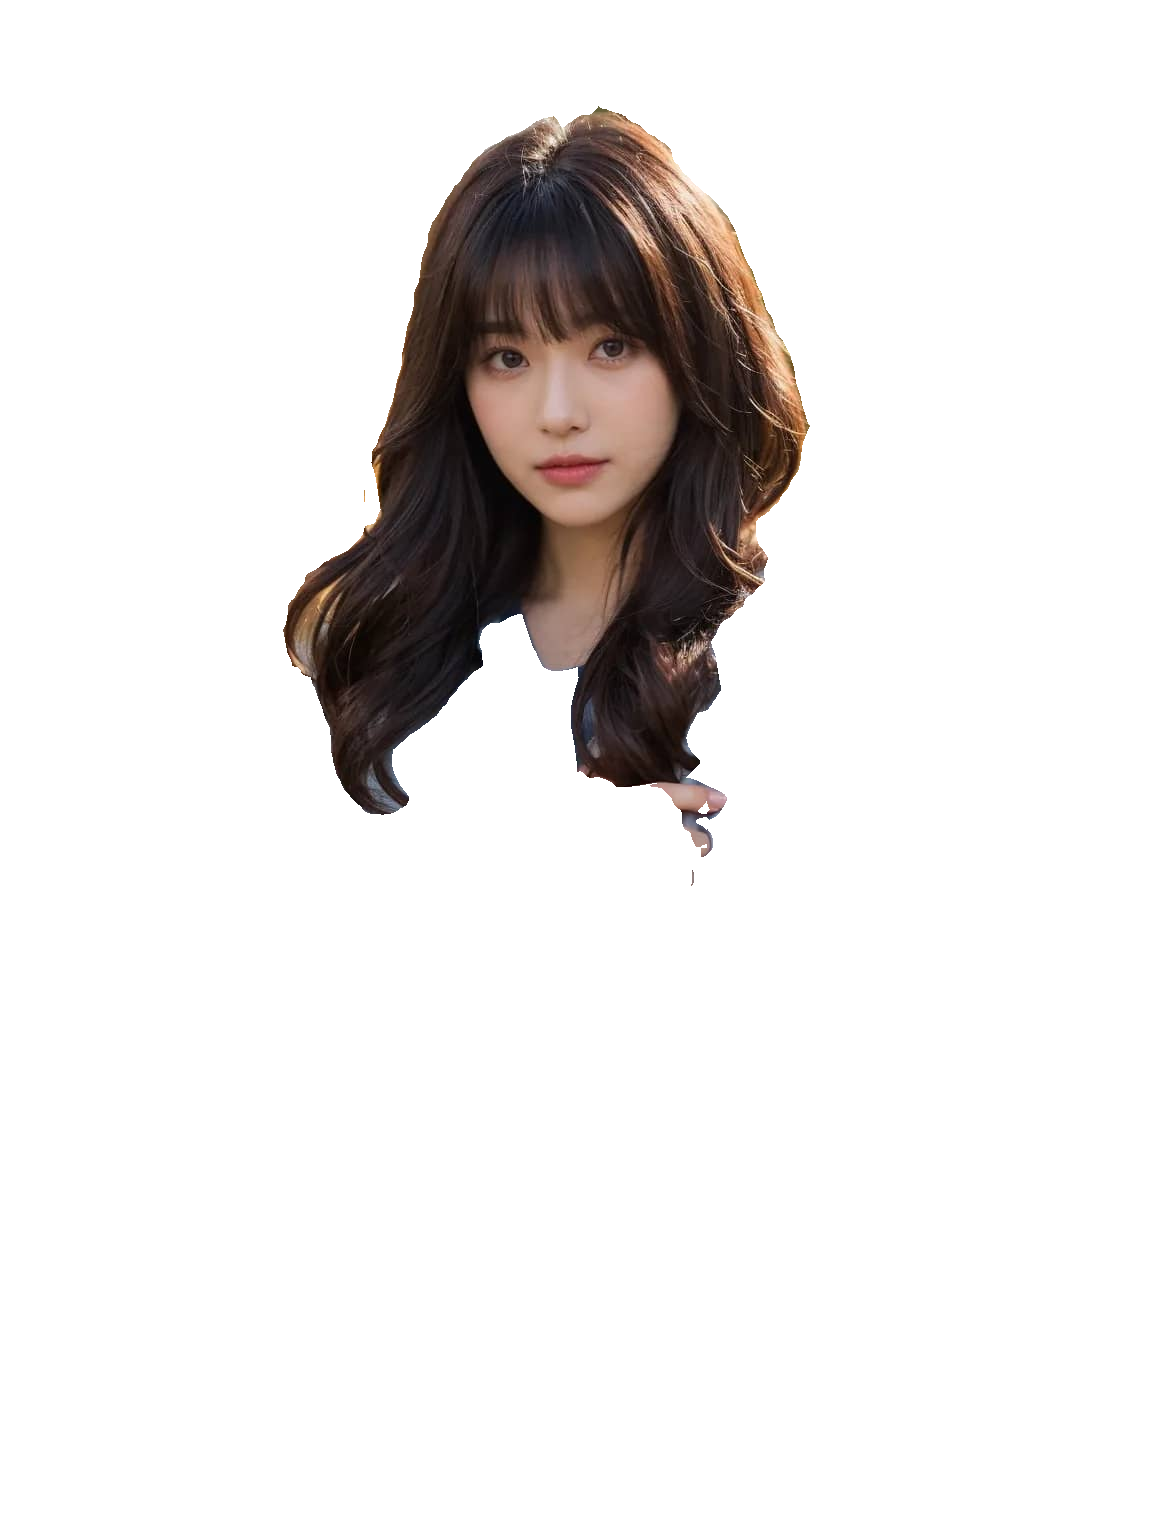
\includegraphics[width=0.24\textwidth]{pictures/example1_step1}
    }
    \caption{基于已给出的点自动填充生成遮罩:\protect\subref{Fig:SegmentPoints}标记后的图像,\protect\subref{Fig:SegmentStep1}生成的遮罩} %注意须使用\protect\subref{}进行标号引用
    \label{Fig:Point} 
\end{figure}

\subsubsection{图像遮罩性能优化}
LRU(Least Recently Used)缓存是一种常用的缓存淘汰算法,用于在有限的缓存空间中管理数据。它的核心思想是优先淘汰最长时间未被使用的数据项。
functools.lru\_cache是python标准库中functools模块提供的一个装饰器,它实现了LRU缓存机制。该装饰器可以非常方便地被添加到任何想要进行缓存的参数可哈希的函数上,自动地保存最近执行的函数调用结果并在后续相同的调用中直接返回缓存的结果,避免重复计算的开销。

由于在本项目中图像遮罩存在一张图片多次调用的特点,本项目使用了LRU缓存实现性能优化。由于python中PIL.Image.Image对象不可哈希,缓存分割结果时将图像转为base64字符串进行映射。
\subsubsection{对自动生成的遮罩进行优化}
由于分割模型性能的限制,生成的原始遮罩可能在某些细节上表现不佳而影响图像编辑模型的结果,因此设计了一个算法对自动生成的遮罩
进行优化。算法5可以根据配置文件的设置,对特定的未被遮罩的部分在遮罩的边缘进行收缩。

\begin{algorithm} 
	\begin{spacing}{1.3}
		\floatname{algorithm}{算法}
		\caption{遮罩优化算法} 
		\label{MaskOptimizationAlgorithm}
		\renewcommand{\algorithmicrequire}{\textbf{输入:}}
		\renewcommand{\algorithmicensure}{\textbf{输出:}} 
			\begin{algorithmic}[1] 
				\Require 原始遮罩$OriginMask$,图像分割结果$SegmentResult$,配置文件$Config$
				\Ensure 优化后的遮罩$OptimizedMask$
				\State 获取遮罩与非遮罩的描边得到像素$EdgePixcels$
				\State 从配置文件和图像分割结果获取$ConfigPixcels$
                \State 仅保留出现在$EdgePixcels$中的$ConfigPixcels$
                \For{$pixcel$ in $ConfigPixcels$}
                    \State Apply MinFilter $Kernel$(in $Config$) in $OriginMask$[$pixcel$]
                \EndFor
                \State 得到优化后的遮罩$OptimizedMask$
			\end{algorithmic}
	\end{spacing}
\end{algorithm}

由于该算法仅会对遮罩边缘上的像素进行卷积且在设计时充分考虑到了内存中像素的存储顺序的原因,虽然需要复杂的处理过程,但经过多次的迭代后算法的时间复杂度降低至$O(mnr)$($m$,$n$表示图片的长宽,$r$表示设置的优化强度)。算法实现的效果如 图4-4 所示,可见在发丝附近遮罩的质量得到了明显的改善。
\begin{figure}[!htbp]
    \centering
    \subfloat[]{ %[]对齐方式,t为top,b为bottom,留空即可
	\label{Fig:MaskOrigin} % 子图1标签名
    	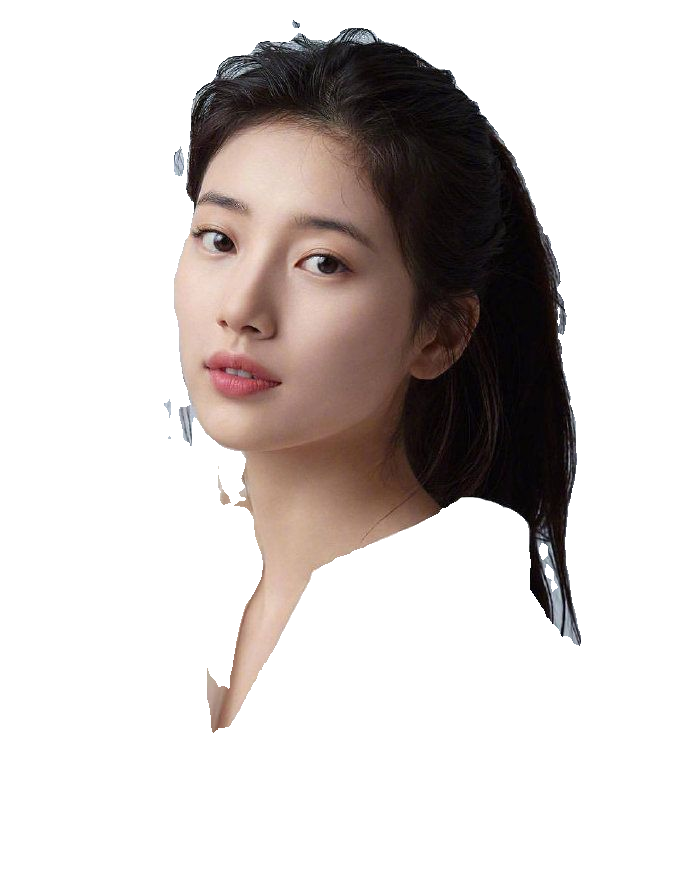
\includegraphics[width=0.24\textwidth]{pictures/example2_step1} %插入图片命令,格式为[配置]{图片路径}
    }
    \quad %空格
    \subfloat[]{
	\label{Fig:MaskOptimized} % 子图2标签名
    	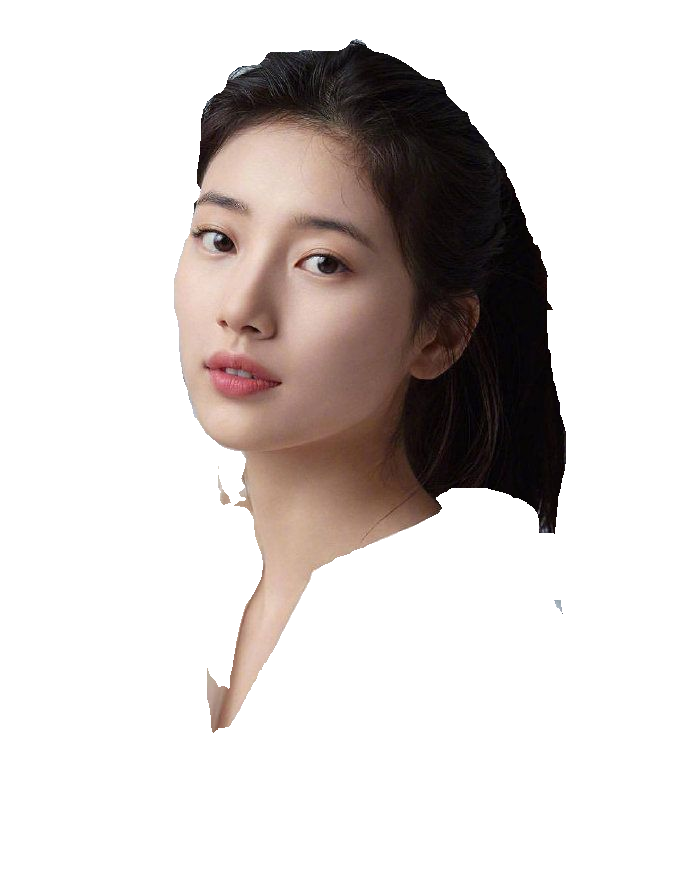
\includegraphics[width=0.24\textwidth]{pictures/example2_step2}
    }
    \caption{遮罩优化结果:\protect\subref{Fig:MaskOrigin}原始遮罩,\protect\subref{Fig:MaskOptimized}算法优化后的遮罩} %注意须使用\protect\subref{}进行标号引用
    \label{Fig:MaskOptimize} % 整个组图的标签名
\end{figure}


\subsection{多模态}
如何打通大语言模型和图像生成模型是本项目的关键。本项目通过特定的prompt和图像分割结果,使用大语言模型生成JSON格式的指令并校验,并支持多轮对话。
用户可有选择性地执行生成的指令或执行全部指令。系统首先会按照给定的规则对指令进行预处理和排序,然后通过指令生成请求参数来调用图像生成模型。多模态任务的实现方式如图4-5。
\buptfigure[width=0.7\textwidth]{pictures/multimodal.png}{多模态实现方式}{multimodal_TMP}

\subsubsection{JSON指令生成}
JSON(JavaScript Object Notation)是一种轻量级的数据交换格式,易于人阅读和编写,同时也易于机器解析和生成。
它基于JavaScript的一个子集,但独立于语言,被广泛应用于许多编程语言中。JSON主要用于网络应用间浏览器与服务器之间的数据传输。
在JSON中,数据以键值对的形式存在,可以表示数组、布尔值、数字、对象或字符串。由于其简洁性和易于交互的特性,JSON已成为Web应用中数据交换的主流技术。
由于JSON应用范围广且大语言模型JSON处理能力较强,本项目采用此格式来承载大语言模型和图像生成模型的联系。

通过特定的prompt和图像分割结果以及用户输入的修改意图,本项目可使用GPT3.5Turbo、GPT4Turbo、
微调后的ChatGLM2-6B生成JSON指令。例:当图像分割结果为Background, Hair, Upper-clothes, Dress, Face, Right-arm,用户输入为
“将背景更换为蓝天白云,将衣服更改为白色的T-shirt”时,生成的JSON指令如 代码4-1 所示。

\begin{lstlisting}[language=Python, caption=生成的指令, label=plus, tabsize=2]  
    [
        {
            "command" : "change",
            "paras" : [ ["Background","Upper-clothes"] , "blue sky, white T-shirt"]
        }
    ]
\end{lstlisting} 

\subsubsection{JSON指令校验}
由于大语言模型生成指令不稳定,需要对生成指令的合规性进行校验。校验规则存储为一个JSON文件,以修改非面部和面部的指令为例,指令校验的算法如 算法6 所示,其中校验规则如 代码 附-1 所示。
\begin{algorithm} 
	\begin{spacing}{1.3}
		\floatname{algorithm}{算法}
		\caption{JSON指令校验算法} 
		\label{JsonCommandCheckAlgorithm}
		\renewcommand{\algorithmicrequire}{\textbf{输入:}}
		\renewcommand{\algorithmicensure}{\textbf{输出:}} 
			\begin{algorithmic}[1] 
				\Require 待校验的指令$JsonCommands$、校验规则$Rules$
				\Ensure 校验后的指令$ValidJsonCommands$
                \For{$Command$ in $JsonCommands$}
                    \If {$Command$ satisfy $Rules$}
                        \State Add $Command$ to $ValidJsonCommands$
                    \EndIf
                \EndFor
			\end{algorithmic}
	\end{spacing}
\end{algorithm}

\subsubsection{多指令处理}
由于一次执行可能会涉及到多个指令,会遇到指令重复、指令优先性等问题,所以会对需要执行的指令进行合并与排序。
指令合并的算法如下:
\begin{algorithm} 
	\begin{spacing}{1.3}
		\floatname{algorithm}{算法}
		\caption{多指令处理算法} 
		\label{JsonCommandsProcessingAlgorithm}
		\renewcommand{\algorithmicrequire}{\textbf{输入:}}
		\renewcommand{\algorithmicensure}{\textbf{输出:}} 
			\begin{algorithmic}[1] 
				\Require 待处理的指令$OriginCommands$、指令合并规则$Rules$、指令优先性$Priority$
				\Ensure 处理后的指令$ProcessedCommands$
                \For{$Command$ in $OriginCommands$}
                    \If {Same $Command$ type already in $ProcessedCommands$}
                        \State Combine $Command$ to the same one in $ValidJsonCommands$ use $Rules$
                    \EndIf
                \EndFor
                \State 根据$Priority$对$ValidJsonCommands$进行排序
			\end{algorithmic}
	\end{spacing}
\end{algorithm}

\subsubsection{图像模型请求参数生成}
图像模型请求参数生成较为复杂,对于某个参数,其可能来源于GUI中可修改的设置,可能来源于指令,可能来源于模版,否则设置为默认参数。
由于每个参数来说,其来源的优先性可能不一致,因此设计了 算法8 来生成图像模型请求参数。
\begin{algorithm} 
	\begin{spacing}{1.3}
		\floatname{algorithm}{算法}
		\caption{图像模型请求参数生成算法} 
		\label{ImageParasGenAlgorithm}
		\renewcommand{\algorithmicrequire}{\textbf{输入:}}
		\renewcommand{\algorithmicensure}{\textbf{输出:}} 
			\begin{algorithmic}[1] 
				\Require 指令$Command$、设置$Settings$、默认参数$Default$、参数来源优先性$PriorityRules$
				\Ensure 图像模型请求参数$Parameters$
                \For{$ParaKey$ in $Parameters$}
                    \State Get $Template$ from $Command$
                    \If {$ParaKey$ found in $Command$ or $Settings$ or $Template$}
                        \State Choose the highest priority source use $PriorityRules$[$ParaKey$]
                    \Else
                        \State Set this parameter to $Default$[$ParaKey$]
                    \EndIf
                \EndFor
			\end{algorithmic}
	\end{spacing}
\end{algorithm}

\subsection{图像修改建议}
本项目提供了根据图像自动生成图像建议的功能。由于传统的大语言模型只能接受文本输入,因此本项目采用了GPT4V来自动生成图像修改建议。

GPT-4V是由OpenAI开发的多模态大型语言模型,是GPT系列基础模型的第四代。该模型具有视觉能力,可以将图片作为输入,进行各种任务,例如描述图片中的幽默、总结截图文本、回答包含图表的考试题目等。

用户通过GUI界面的Advise按键,可以生成建议并将其转换为指令。

\section{Middleware的构建} % 641 + 94 + 19 = 754
在本项目中,Middleware作为核心组件,通过整合来自不同平台的API,为GUI提供了统一且易于接入的API服务。
其整合了多个图像生成和大语言语言模型,通过统一的接口设计,使得GUI能够方便地调用所需的功能。
此外,Middleware采用了Golang语言和Beego框架,不仅保证了API服务的高并发处理能力和稳定性,
还通过模块化的设计提高了系统的可维护性和可扩展性。主要API服务包括Stable Diffusion和DALL-E2模型、
图像分割模型,以及多种大语言模型。这样的架构设计不仅优化了开发效率,也确保了系统的稳定运行和长期发展。
\subsection{对多个平台的API进行配置和整合}
Middleware通过整合不同平台如图像生成模型、语言模型等的API,使得GUI开发者可以通过一个统一的接口调用多种功能。
这种整合不仅包括API的聚合,还涉及统一API调用的风格和路由规范,不仅保证了API服务的高稳定性和可靠性,还便于日后的维护和扩展。例如,无论是调用ChatGLM2-6B模型还是多种GPT模型,
GUI都能通过相同的结构化请求方式访问不同的服务。


\subsection{使用Beego框架提供API服务}
本项目使用beego框架构建了Middleware组件提供了多个API服务,以便GUI可以高效地使用各种模型和工具。
$PostSDTxt2Img$和$PostSDImg2Img$是通过Stable Diffusion模型来生成或修改图像的API,这使得用户能够通过简单的API调用,进行复杂的图像生成和编辑操作。$GetLoras$这个API用于获取Stable Diffusion模型可用的LoRA模型列表。
$PostDALLE2Edit$利用DALL-E2模型修改图片,这进一步扩展了图像处理的能力,在Stable Diffusion模型不可用时作为替代。
$PostHuggingFaceImgSegment$ API通过可在部署在本地的分割模型不可用时通过调用Hugging Face上的图像分割模型API来实现图像分割。
在文本处理方面,$PostGPT3Dot5Turbo$、$PostGPT4Turbo$和$PostGPT4V$等API利用OpenAI的不同版本GPT模型来处理指令理解和生成任务,$PostChatGLM2\_6B$可调用微调后的ChatGLM2-6B模型来进行指令生成。

\section{LLM的微调} % 1820 + 119 + 197 = 2136
大语言模型(LLM)的微调是一种在预训练模型基础上通过特定数据集进一步训练的过程,用于优化模型在特定任务或场景中的表现。特别是对于参数量较小的LLM,微调不仅可以提升其性能,还能增强其针对具体任务的适应性和泛化能力。
微调的一个主要优势是性能提升,即使是较小的模型,通过针对性的微调,可以在特定任务上实现甚至超过大型模型未经微调时的性能,可见微调能够根据具体需求调整模型的行为,使其更加专注于特定的输出目标。
微调技术提供了一种有效途径,通过少量的定制化数据提升模型的应用性能,特别是在参数量较小的模型中,这种优势尤为显著。

原始的ChatGLM2-6B模型已经通过大规模数据预训练,具备了强大的语言理解和生成能力,但受制于参数量较小,其在本项目需要高精准度的指令生成任务上表现不佳,因此本项目通过自动生成并进行筛选的高质量指令生成微调数据集对ChatGLM2-6B进行微调以进一步提升模型在指令生成任务的表现。

本项目利用开源项目LLaMA-Factory\footnote{https://github.com/hiyouga/LLaMA-Factory}和本项目中自动生成的指令生成任务数据集对ChatGLM2-6B模型进行微调。
\subsection{LLM微调数据集生成与性能评估方法}
\subsubsection{微调数据集生成}
在大语言模型(LLM)的微调过程中,数据集的功能和作用至关重要。微调数据集不仅提供了模型训练所需的具体数据,还直接影响了模型微调后的性能和适应性。
对于参数量较小的模型,高质量的微调数据集尤其重要,因为这些模型通常缺乏足够的参数量来从大规模数据中学习复杂的特征。通过高质量的微调数据集,参数量较小的大语言模型可以有效地提高这些模型的学习效率和最终性能。
构造高质量的微调数据集涉及两个关键步骤:数据收集和数据预处理。数据收集需要确保获得足够多的、具有代表性的数据,这些数据能够覆盖模型在实际应用中可能遇到的各种情况。数据预处理是将收集到的原始数据转换成模型可以直接处理的格式,这可能包括数据清洗、特征提取、标签编码等。

由于没有适用于本任务的开源数据集,本项目尝试建立一个自动化工作流程,
通过利用ATR Dataset\footnote{https://github.com/lemondan/HumanParsing-Dataset}调用多个模型和一定的校验规则来生成所需的数据并整合为一个数据集。数据集生成的流程如 图4-6。
同时,在系统使用过程中产生的数据可设置是否保存,这些数据也会在运行数据集生成脚本添加到数据集中。
\buptfigure[width=0.65\textwidth]{pictures/dataset.png}{数据集自动生成流程}{dataset_TMP}

通过建立的自动化工作流程,本项目创建了一个包含3000个样本的数据集,数据集中的每一项数据都经过合法性校验以保证数据集的质量。数据集的格式满足LLaMA-Factory的要求并可使用此数据集对ChatGLM2-6B进行微调。
\subsubsection{LLM指令生成任务性能评估方法}
性能评估是大语言模型(LLM)开发和应用的关键环节,尤其是在模型的实用性和可靠性方面。有效的评估方法可以帮助研究者和开发者了解模型在特定任务上的表现,从而进行进一步的优化和调整。

由于需要一种直观的性能评估方法来对不同的大语言模型在指令生成任务上的性能进行评估,本项目采用生成指令的合法率对不同的大语言模型在指令生成任务上的性能进行评估。


\subsection{ChatGLM2-6B针对指令生成任务的微调}
LoRA: Low-Rank Adaptation of Large Language Models\cite{hu2021lora}这篇论文提出了一种新颖且高效的$LoRA$微调方法,用于微调大型预训练语言模型以适应特定任务。传统的微调方法往往需要重新训练模型的所有参数,而全参数训练的方法在模型参数规模庞大时需要巨大的量。算法主要通过在Transformer模型的每一层中注入低秩的分解矩阵来更新权重,而不改动预训练的权重,其具体算法描述见算法9。
\begin{algorithm}
	\begin{spacing}{1.3}
		\floatname{algorithm}{算法}
		\caption{LoRA: 大型语言模型的低秩适配} 
		\label{LoRA_model}
		\renewcommand{\algorithmicrequire}{\textbf{输入:}}
		\renewcommand{\algorithmicensure}{\textbf{输出:}} 
			\begin{algorithmic}[1] 
				\Require 预训练权重矩阵 $W_0 \in \mathbb{R}^{d \times d}$, 输入 $x$, 秩 $r$
				\Ensure 调整后的输出 $h$
				\State 初始化低秩矩阵 $A \in \mathbb{R}^{r \times d}$ 和 $B \in \mathbb{R}^{d \times r}$
				\State 冻结预训练权重 $W_0$
				\For {对于每个训练步骤:}
				    \State 计算更新矩阵 $\Delta W = BA$
				    \State 应用更新:$W = W_0 + \Delta W$
				    \State 计算输出:$h = Wx$
				\EndFor
				\State 优化参数 $A$ 和 $B$ 以最小化损失函数
			\end{algorithmic}
	\end{spacing}
\end{algorithm}


本项目使用生成的指令生成任务数据集结合$LoRA$方法,通过开源项目LLaMA-Factory\footnote{https://github.com/hiyouga/LLaMA-Factory}对ChatGLM2-6B模型进行微调。
LoRA微调在大语言模型上的训练损失随训练步数变化的情况如 图4-7所示。从图中可以看出,最初损失值很高,但随着训练步数的增加,损失值迅速下降,特别是在前50步之内下降最为显著。
在经过约50步之后,损失下降的速度开始放缓,但仍然持续下降,表明模型继续从训练数据中学习。在约200步之后,损失曲线趋于平缓,说明模型已经接近收敛,额外的训练步骤在减少损失方面的效果变得有限。
图中还展示了一个平滑处理的损失曲线,更清晰地显示了训练过程的整体趋势,而不是每一步的波动。
\buptfigure[width=0.6\textwidth]{pictures/training_loss}{step-loss图}{pic_step_loss}

\subsection{各个LLM在本任务下的性能评估}
结合本项目的LLM指令生成任务性能评估方法,本项目对不同的大语言模型进行了指令生成任务性能评估。各个模型的性能表现如 表4-2 和 图4-8 所示。
\begin{bupttable}{LLM 指令生成性能}{table_llm_scores}
    \begin{tabular}{|l|l|l|}
        \hline \textbf{模型} & \textbf{测试样本数} & \textbf{合格率} \\
        \hline GPT3.5Turbo & 100 & 97\% \\
        \hline GPT4Turbo & 100 & 99\% \\
        \hline ChatGLM2-6B(Origin) & 100 & 6\% \\
        \hline ChatGLM2-6B(LoRA trained 50 steps) & 1000 & 19.1\% \\
        \hline ChatGLM2-6B(LoRA trained 60 steps) & 1000 & 43.7\% \\
        \hline ChatGLM2-6B(LoRA trained 80 steps) & 1000 & 77.8\% \\
        \hline ChatGLM2-6B(LoRA trained 100 steps) & 1000 & 88.1\% \\
        \hline ChatGLM2-6B(LoRA trained 150 steps) & 1000 & 93.9\% \\
        \hline ChatGLM2-6B(LoRA trained 200 steps) & 1000 & 95.8\% \\
        \hline ChatGLM2-6B(LoRA trained 250 steps) & 1000 & 95.2\% \\
        \hline ChatGLM2-6B(LoRA trained 300 steps) & 1000 & 96.7\% \\
        \hline
    \end{tabular}
\end{bupttable}

\buptfigure[width=0.7\textwidth]{pictures/5e56eff9-d478-4134-9d08-b1084e92f408}{LLM 指令生成性能}{model_performance_TMP}


可观察到原始的ChatGLM2-6B模型在未经过微调时,在指令生成任务中的合格率仅为6\%。
这一低下的性能表现暴露了ChatGLM2-6B模型在没有针对性训练的情况下难以完成需要高紧准度指令生成任务。
通过使用LoRA方法进行微调,模型性能随着微调步骤的增加显著提升。当微调步骤增至80步时,合格率提升至77.8\%;
而在经过200步的微调后,合格率达到95.8\%,并在300步训练后稳定在96\%左右。
与ChatGLM2-6B相比,GPT3.5Turbo和GPT4Turbo在无需额外训练的情况下即可达到分别为97\%和99\%的高合格率。

\section{Stable Diffusion及扩展的使用} % 439 + 106 + 37 = 582
Stable Diffusion是一种基于深度学习的图像生成模型,能够根据文本描述生成高质量的图像。该模型利用条件生成技术,允许用户通过简单的文本指令来引导图像的生成过程。这种技术在艺术创作、媒体娱乐、广告以及数字营销等多个领域显示了广泛的应用潜力。

除了Stable Diffusion的基础功能外,本项目还集成了多个扩展,如ControlNet和roop。ControlNet允许用户对生成的图像进行更精确的控制,通过这种方式ControlNet增强了图像的细节质量和一致性,使生成的图像更贴近用户的具体需求。
roop专注于提供面部替换功能,这一功能特别适用于需要在图像中修改人物面部特征的场景。roop通过简单的操作接口,使得用户能够轻松地将一张人脸图像替换到另一张人脸上,而不需要复杂的图像处理知识背景。

sd-webui-controlnet\footnote{https://github.com/Mikubill/sd-webui-controlnet}使用了ControlNet的原理,
旨在增强原有 Stable Diffusion 模型的图像生成控制能力。通过集成一个额外的控制网络(ControlNet),
允许用户精确指导图像的具体内容,显著提升了生成图像的细节质量和一致性。

sd-webui-roop\footnote{https://github.com/s0md3v/sd-webui-roop}基于DeepFake\cite{van2021deepfake},
允许用户在图片中进行面部替换,简化了面部交换的过程,无需训练特定的模型,大大降低了使用复杂度。

系统还提供了丰富的参数调整选项,如调整噪声去除强度。这些功能为用户提供了广泛的自定义空间,可以根据具体的应用场景调整生成效果,以满足不同的视觉表达需求。Stable Diffusion模型及其扩展的结合使用,为本项目的图像编辑方面提供了强大的功能和更高的灵活性。

\subsection{Stable Diffusion API的使用}
本项目通过将开源项目stable-diffusion-webui\footnote{https://github.com/AUTOMATIC1111/stable-diffusion-webui}部署在揽睿星舟机器学习平台\footnote{https://www.lanrui-ai.com},通过API来调用Stable Diffusion模型,
主要使用的参数见表4-3。
\begin{bupttable}{主要使用的Stable Diffusion webui img2img API 参数}{sdapi_params}
    \begin{tabular}{|l|l|l|}
        \hline \textbf{参数} & \textbf{描述} & \textbf{形式} \\
        \hline \texttt{prompt} & 输出图像的期望修改或主题 & str \\
        \hline \texttt{negative\_prompt} & 生成图像中应避免的内容 & str(base64 Image) \\
        \hline \texttt{mask} & 选择性编辑或生成的区域的图像遮罩 & str \\
        \hline \texttt{inpainting\_fill} & 修补时的填充方法 & int \\
        \hline \texttt{inpaint\_full\_res} & 是否在图像的全分辨率下应用修补 & bool \\
        \hline \texttt{inpaint\_full\_res\_padding} & 使用全分辨率时修补区域周围的填充 & int \\
        \hline \texttt{inpainting\_mask\_invert} & 是否反转修补遮罩 & bool \\
        \hline \texttt{mask\_blur} & 遮罩边缘的模糊量 & float \\
        \hline \texttt{denoising\_strength} & 去噪强度 & float \\
        \hline \texttt{sampler\_index} & 采样算法 & str \\
        \hline \texttt{seed} & 初始化随机数生成器的值 & int \\
        \hline \texttt{steps} & 生成图像时的步骤数 & int \\
        \hline \texttt{width} & 输出图像的宽度 & int \\
        \hline \texttt{height} & 输出图像的高度 & float \\
        \hline \texttt{cfg\_scale} & 输入提示的权重 & float \\
        \hline \texttt{restore\_faces} & 是否修复生成图像中的面部 & bool \\
        \hline \texttt{alwayson\_scripts} & 插件参数 & dict \\
        \hline
    \end{tabular}
\end{bupttable}

\subsection{ControlNet的使用及效果}
sd-webui-controlnet\footnote{https://github.com/Mikubill/sd-webui-controlnet}是一个用于stable-diffusion-webui的扩展,允许用户通过添加额外的条件来控制扩散模型的行为,从而增强生成图像的精确度和控制性。这一扩展可以实时添加到原始的 Stable Diffusion 模型中,不需要进行合并处理。
本项目使用该插件以保持原始图像的主要轮廓和布局不受改变,其实现的效果如图4-9。
\begin{figure}[!htbp]
    \centering
    \subfloat[]{ %[]对齐方式,t为top,b为bottom,留空即可
	\label{Fig:InitImage} % 子图1标签名
    	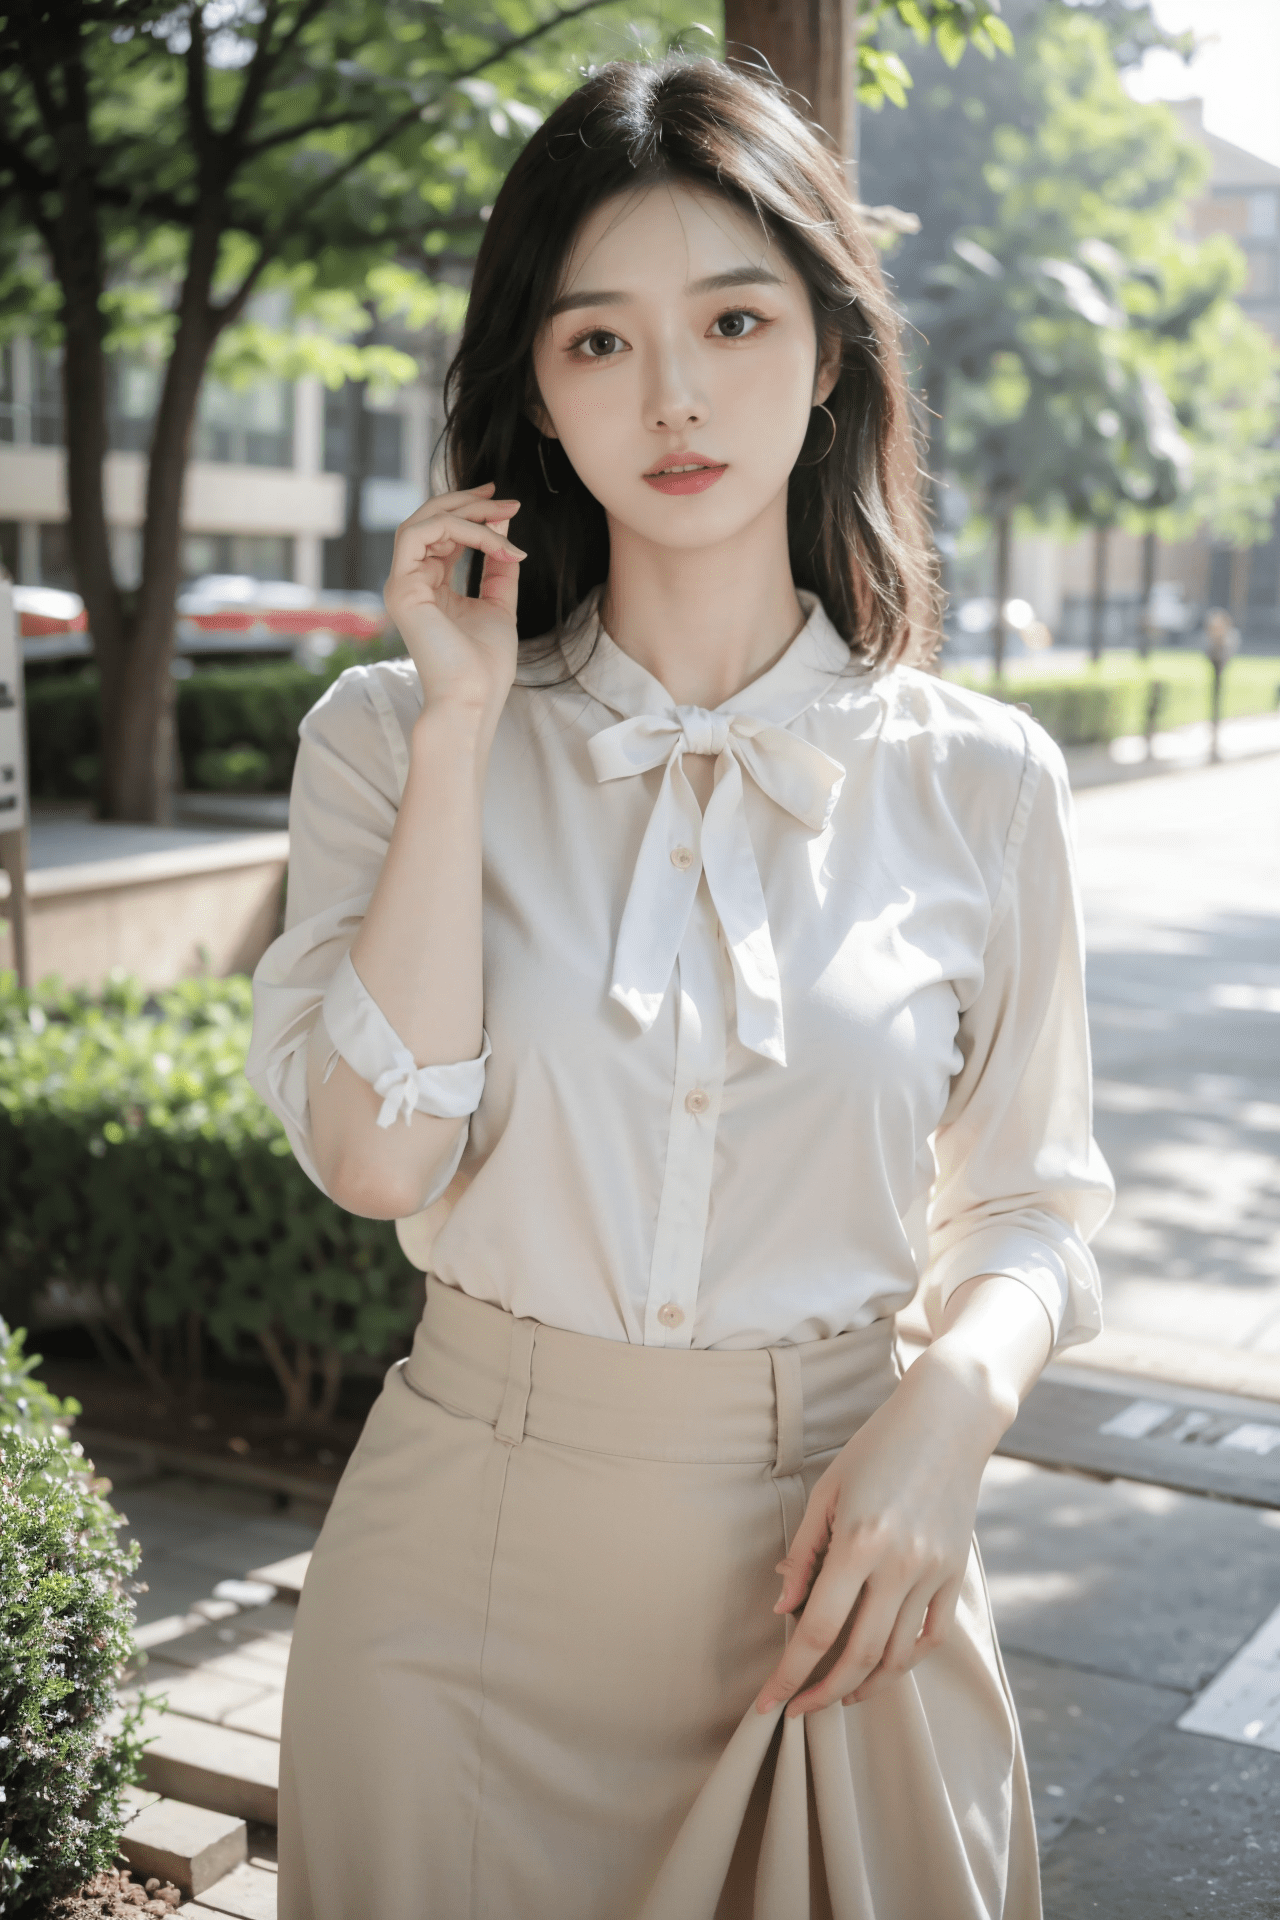
\includegraphics[width=0.24\textwidth]{pictures/253cdd65-d088-4fd2-9ccf-bcb85e909ada} %插入图片命令,格式为[配置]{图片路径}
    }
    \quad %空格
    \subfloat[]{ %[]对齐方式,t为top,b为bottom,留空即可
	\label{Fig:NoCanny} % 子图1标签名
    	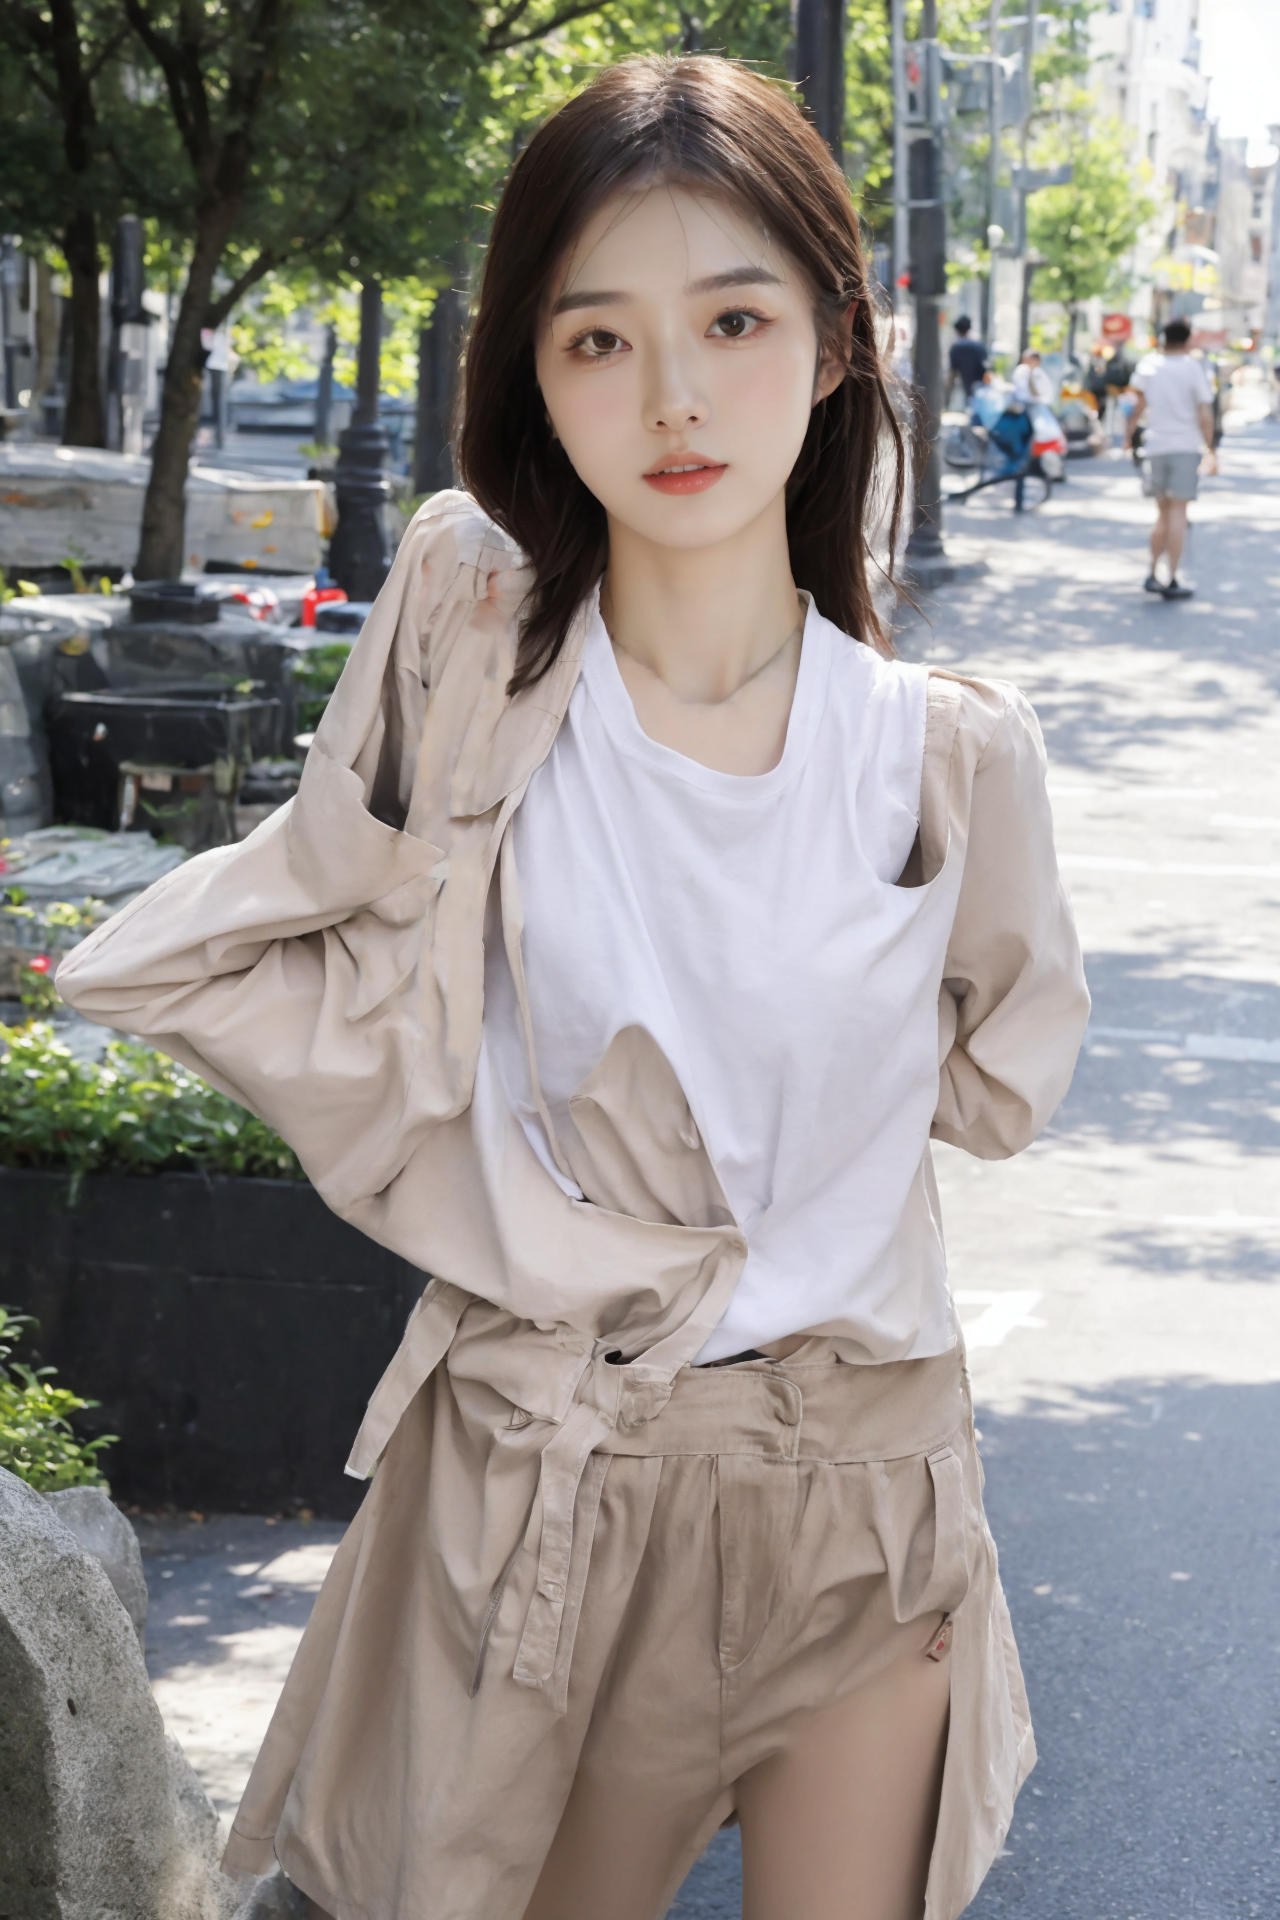
\includegraphics[width=0.24\textwidth]{pictures/00010-43719289} %插入图片命令,格式为[配置]{图片路径}
    }
    \quad %空格
    \subfloat[]{
	\label{Fig:Canny} % 子图2标签名
    	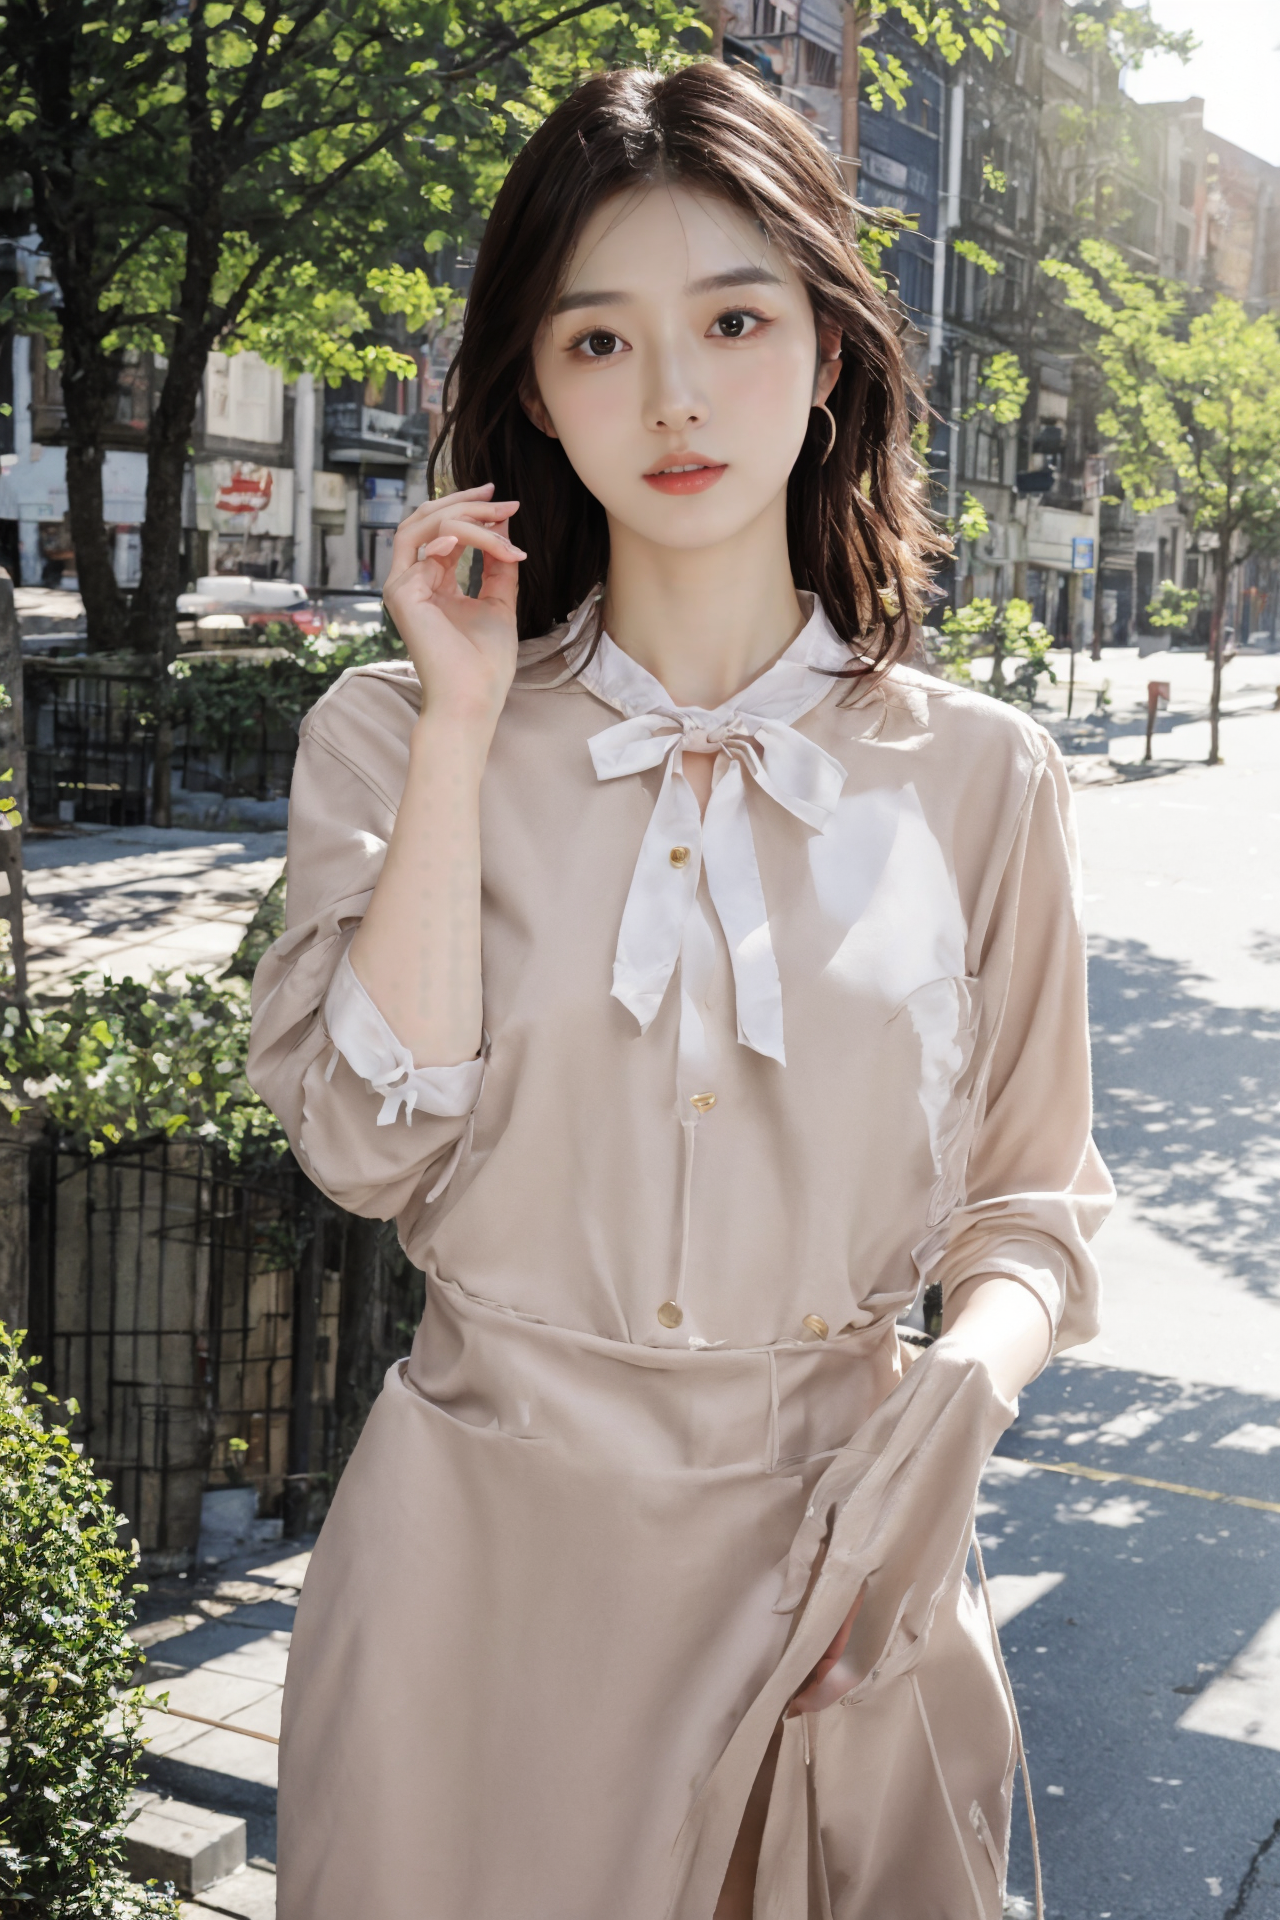
\includegraphics[width=0.24\textwidth]{pictures/00013-743295153}
    }
    \caption{ControNet效果:\protect\subref{Fig:InitImage}原始图像,\protect\subref{Fig:NoCanny}未使用ControlNet,\protect\subref{Fig:Canny}使用ControlNet} %注意须使用\protect\subref{}进行标号引用
    \label{Fig:ControlNet} % 整个组图的标签名
\end{figure}
\subsection{Roop的使用及效果}
roop\footnote{https://github.com/s0md3v/sd-webui-roop}是一个用于stable-diffusion-webui的扩展,提供面部替换的功能。这个扩展需要一张原始图像和目标图像,并能将原始图像的面部替换到目标图像上。
其实现的效果如图4-10。
\begin{figure}[!htbp]
    \centering
    \subfloat[]{ %[]对齐方式,t为top,b为bottom,留空即可
	\label{Fig:init} % 子图1标签名
    	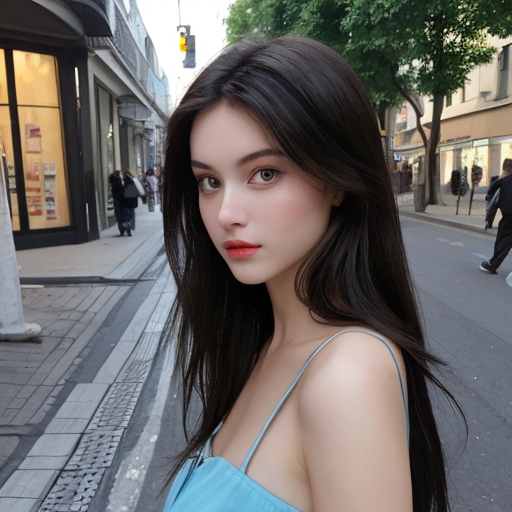
\includegraphics[width=0.26\textwidth]{pictures/00003-736437415} %插入图片命令,格式为[配置]{图片路径}
    }
    \quad %空格
    \subfloat[]{
	\label{Fig:target} % 子图2标签名
    	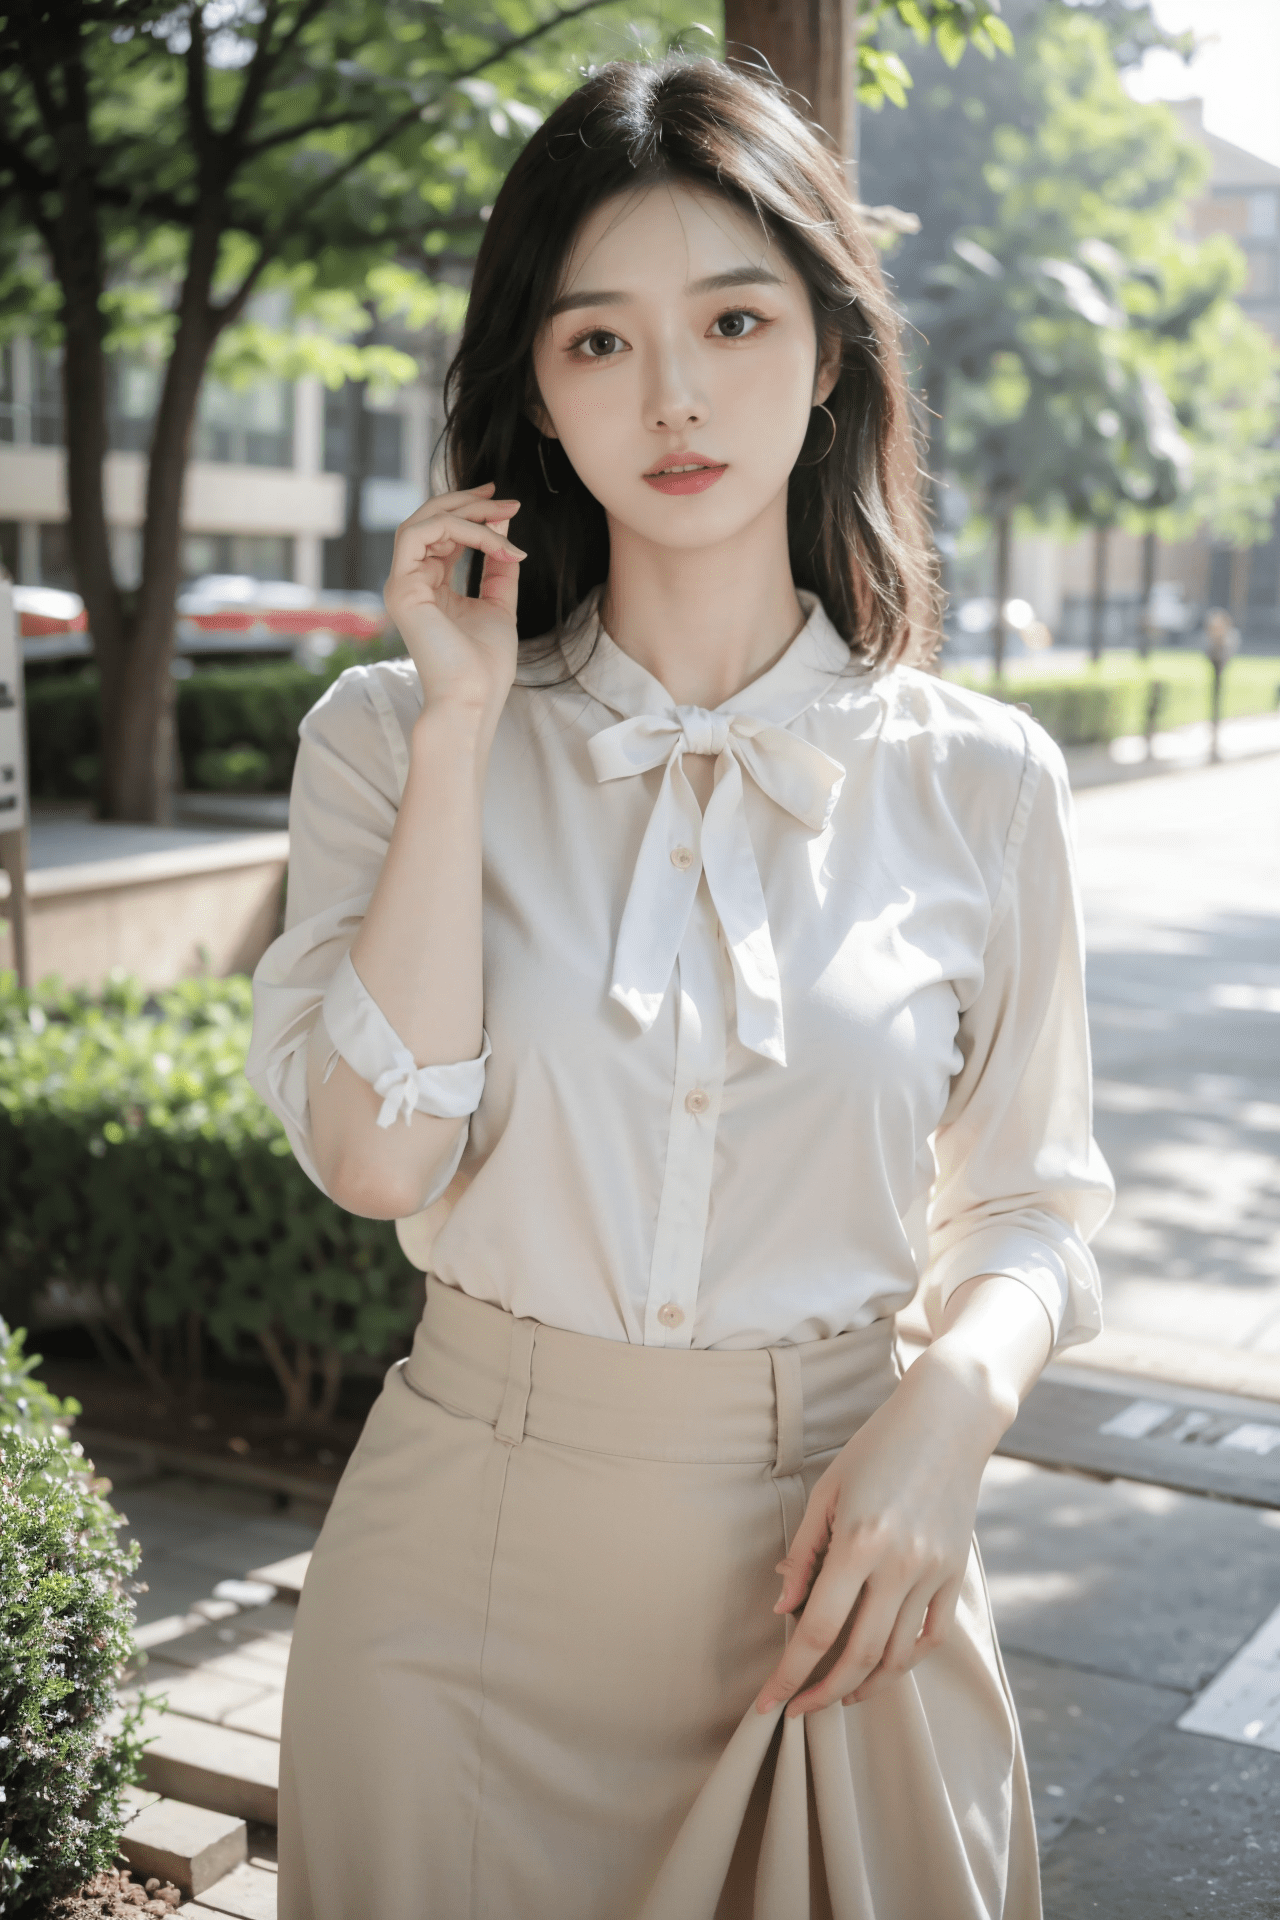
\includegraphics[width=0.2\textwidth]{pictures/253cdd65-d088-4fd2-9ccf-bcb85e909ada}
    }
    \quad %空格
    \subfloat[]{
	\label{Fig:result} % 子图3标签名
    	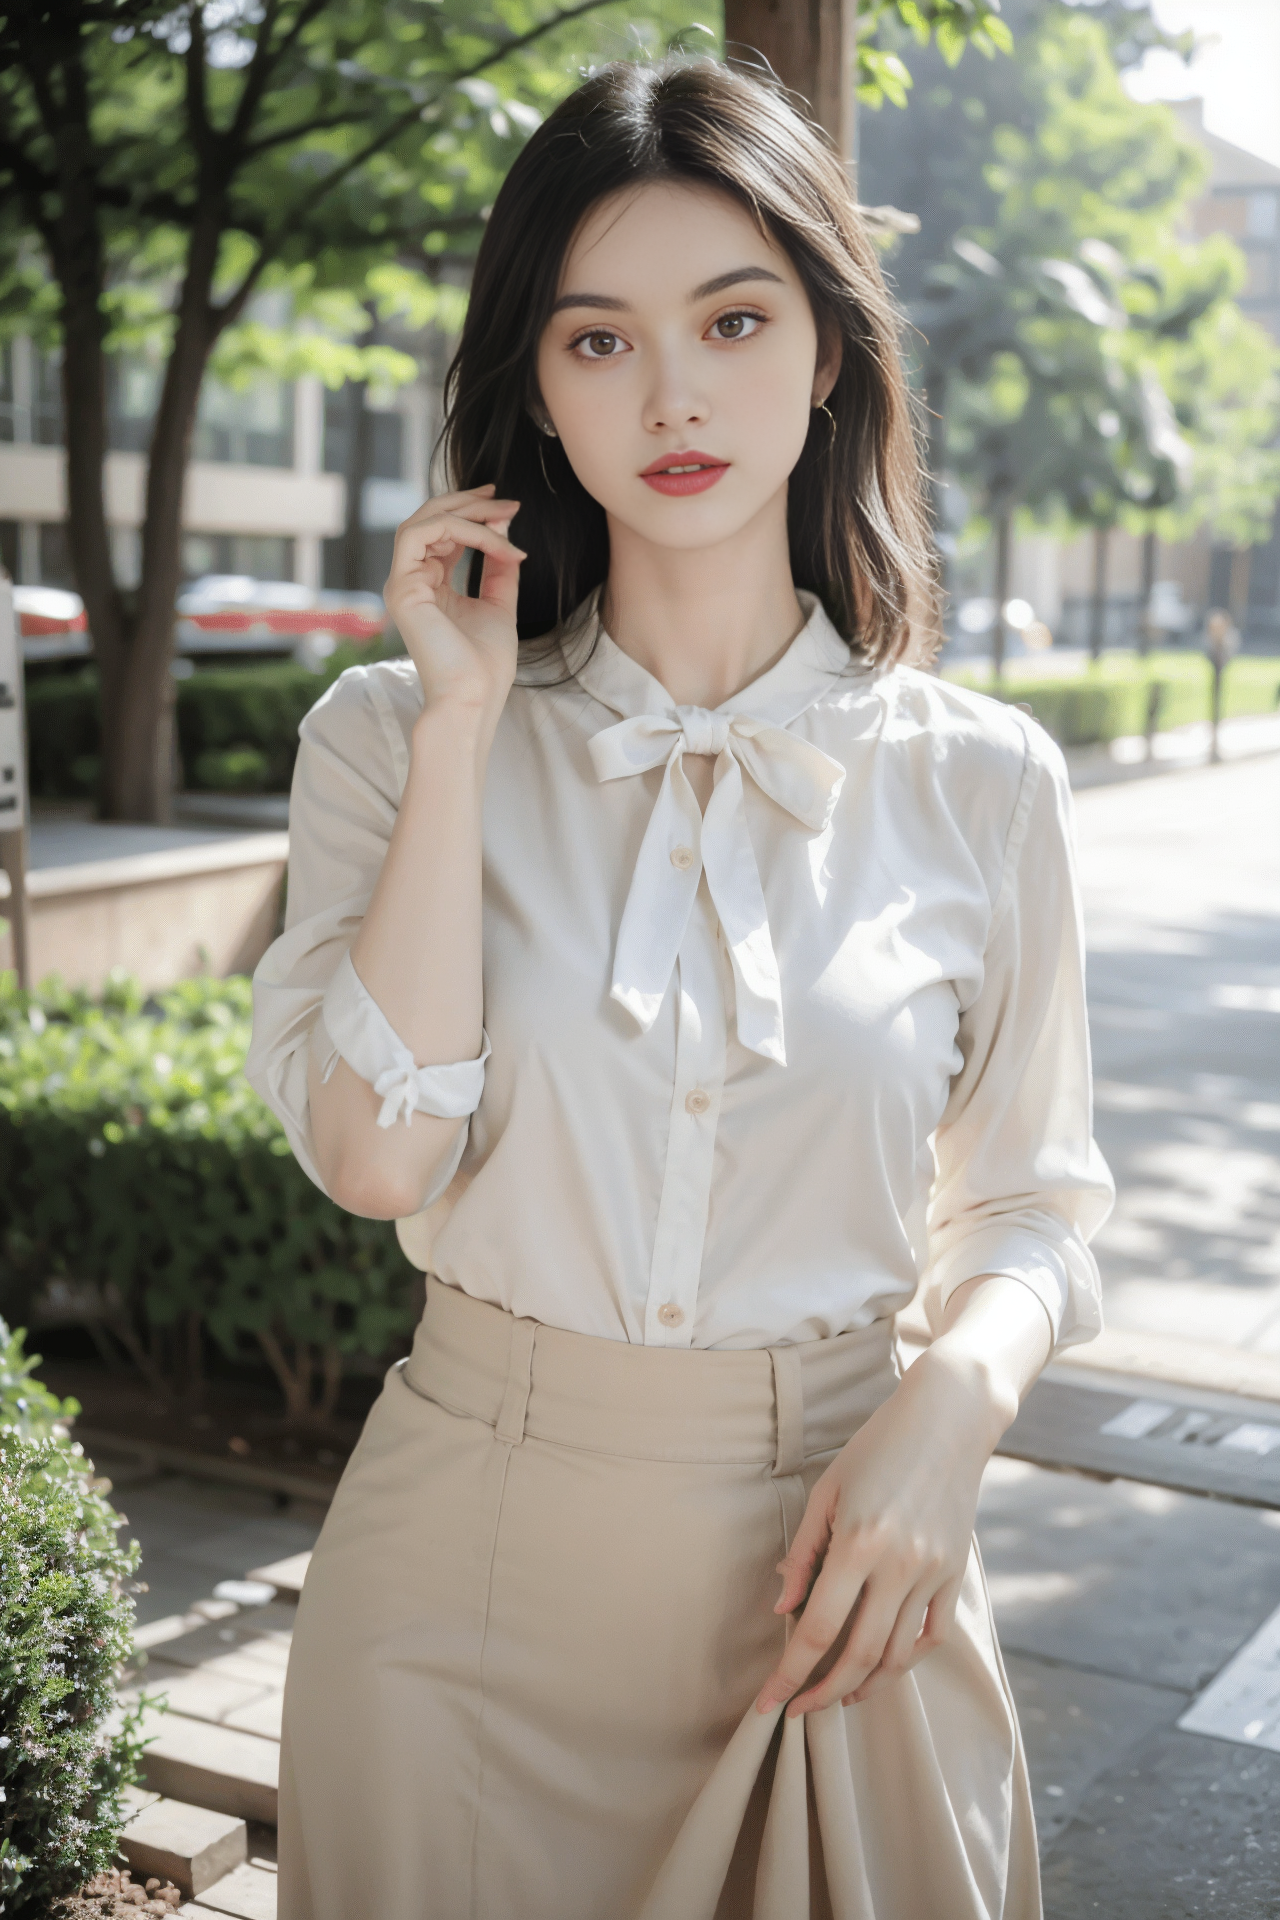
\includegraphics[width=0.2\textwidth]{pictures/image-10}
    }
    \caption{roop效果:\protect\subref{Fig:init}原始图像,\protect\subref{Fig:target}目标图像,\protect\subref{Fig:result}结果} %注意须使用\protect\subref{}进行标号引用
    \label{Fig:Roop} % 整个组图的标签名
\end{figure}

\section{本章小结}
本章中详细介绍了基于大语言模型(LLM)的交互式多模态图像编辑系统的设计与实现。本章首先阐述了图形用户界面(GUI)的构建过程,接着描述了中间件的开发过程,还探讨了LLM的微调技术及其在本系统中的应用,以及如何利用Stable Diffusion模型和其他技术来增强图像编辑的功能。这些元素共同构成了一个高效、直观的图像编辑系统。
\chapter{系统实现效果与使用} % 1196
系统实现的核心在于其高度集成的图形用户界面(GUI),该界面不仅简洁易用,还充分支持复杂的图像处理操作。GUI设计考虑了用户的操作习惯,提供了直观的图像上传、编辑和预览功能。用户可以通过简单的点击和拖拽操作,实现图像的上传和编辑。GUI还集成了多个图像生成模型和大语言模型并提供控制选项,如模型选择、参数调整等,使用户能够根据具体需求调整图像处理流程。
\section{系统实现效果}
系统实现了一个简单易用的GUI,可通过特定端口进行访问。GUI的总体效果如图5-1所示。
\buptfigure[width=0.8\textwidth]{pictures/gui}{GUI总体效果}{gui_TMP}

可使用GUI的Auto模块进行LLM微调数据生成和LLM指令生成任务性能测试,其实现效果如图5-2所示。
\buptfigure[width=0.7\textwidth]{pictures/gui_auto}{Auto模块}{gui_auto_TMP}

可使用GUI的Manual模块查看GUI使用方法,其实现效果如图5-3所示。
\buptfigure[width=0.7\textwidth]{pictures/gui_manual}{Manual模块}{gui_manual_TMP}

使用GUI进行基于LLM的交互式图像编辑时,系统主要模块效果如图5-4所示。
\buptfigure[width=0.6\textwidth]{pictures/gui_multimodal}{交互式图像编辑}{gui_multimodal_TMP}

\section{系统使用方法}
\subsection{系统部署}
本项目提供了Docker、Kubernetes等多种常用的项目部署方式以适应不同的用户需求和操作环境。
如果选择通过Docker进行部署,用户可以根据需求选择不同的镜像。通过运行命令docker run --name multimodal -p 27777:80 binciluo/multimodal:latest,可以在本地部署图像分割模型。
如果希望通过Hugging Face API使用图像分割功能以在性能受限的设备上运行,则可以使用命令docker run --name multimodal -p 27777:80 binciluo/multimodal:mini\_latest。
部署完成后,用户可通过访问本地地址127.0.0.1:27777来使用服务。
对于Kubernetes部署,用户需要先切换到包含Kubernetes配置文件的目录,使用kubectl apply -f pod.yaml命令部署服务(对于使用Arm架构的用户,则需使用kubectl apply -f pod\_arm.yaml)。非Linux用户需运行kubectl port-forward mm-service-pod -n default 27777:27777以访问服务。服务可通过127.0.0.1:27777地址访问。

项目还支持本地直接运行。用户需要先安装Golang和Beego框架,然后安装Python所需的依赖包。首先安装Golang,接着通过命令go install github.com/beego/bee/v2@latest安装Beego,然后运行pip install -r gradio\_web/requirements.txt安装Python依赖。最终,通过运行脚本runner.sh启动服务,或者设置环境变量SEG\_MODEL\_ENV='local'并运行runner\_local.sh脚本以在本地使用图像分割模型。

\subsection{GUI使用说明}
1. 上传基础图像:
您可以上传您的基础图像,或者使用在Base Image中的Examples提供的示例图像。图像上传后,系统会自动地进行图像分割任务并在Chat界面显示分割结果。

2. 与LLM对话
您可以就如何编辑基础图像提出您的看法,或者使用在Chat中的Examples提供的示例。LLM的回复会被识别是否含有指令,若有指令存在则会对指令进行提取并自动添加至Operation Board中。

3. 选择指令来修改基础图像
您可以在Operation Board中选择单个或多个指令,并有两个按钮可供选择:Exec Selected Commands和Exec All Commands。Exec Selected Commands会执行选中的指令,而Exec All Commands会执行所有指令。系统会对这些指令进行合并与排序等预处理,然后生成对应的参数向图像编辑模型发起请求。

4. 预览编辑后的图像并设置为基础图像
您可以在Edited Image标签中预览编辑后的图像,并点击Set as Base Image将其设置为新的基础图像。

5. 替换面部
您可以使用Edit Image标签中的Change Face功能,将基础图像的面部(仅支持单一面部)替换为特定面部。

6. 编辑遮罩
如果您对自动生成的遮罩不满意,可以在Edit Image标签的Editor中手动编辑,然后重新运行之前的指令。

7. 检查服务器状态
您可以点击Check Server Status来确认所有服务是否可用。系统会在大约三秒后弹出提示框显示哪些服务目前不可用。

8. 自动生成LLM微调数据
您可在Auto模块中的Gen Data选择图片,输入OpenAI的API Key并指定生成数量和线程数以生成LLM微调数据。

9. 对LLM指令生成合格率进行测试
您可在Auto模块中的Test LLM选择测试集并指定测试样本数量和线程数以对LLM指令生成合格率进行测试。

\section{本章小结}
在本章中,我们展示了基于LLM的交互式多模态图像编辑系统的实际运行效果和用户使用方法,提供了详细的用户操作指南,确保用户能够充分利用系统功能进行图像编辑。

\chapter{项目管理与维护} % 1755 + 149 + 26 = 1930
\section{代码管理}
Git是一个开源的分布式版本控制系统,其允许多个开发者在共同的代码基础上工作,同时能够追踪和记录所有文件的历史变更,
兼具高性能与灵活性。Git能处理从小到大的项目,让开发者能够在本地机器上工作,并保持代码的多个版本,
以便在不同的分支上进行试验和开发新功能而不影响主代码库。

GitHub\footnote{https://github.com}是一个基于Git的代码托管和协作平台,其为开发者提供了一个强大而便捷的环境来管理代码和协作,
不仅能够追踪和记录代码的变更历史以确保代码的完整性和回溯能力,还能通过分支管理支持多线程的工作流以允许多个开发者同时推进不同的功能。
GitHub的pull请求机制促进了团队成员之间的代码审查和讨论,不仅提高了代码质量也加强了团队协作能力。GitHub的集成系统支持持续集成和持续部署流程,
与各种开发工具链的无缝连接,使得项目管理更加高效。由于其承载了众多开源项目,GitHub成为开发者的一个展示和交流的平台,促进了知识共享和技术交流。

为了便于进行代码管理和版本控制,本项目在GitHub上创建了一个仓库\footnote{https://github.com/BinciLuo/multimodal-service},结合GitHub的其他功能,将其发展成了功能完整、文档详细的开源项目。


\section{自动化测试}
自动化测试是一种利用软件来控制执行测试的过程,其能自动比较实际的运行结果与预期结果来验证被测软件功能是否符合预期。
自动化测试的主要功能是提高测试的效率和覆盖率,其可以快速地执行大量的测试用例,并且可以反复运行这些测试,在软件开发的早期发现缺陷,从而减少修复缺陷的成本并确保软件在开发迭代中未引入错误。
自动化测试还可以将测试人员从繁琐的手动测试工作中解脱出来,使他们有更多时间专注于更复杂的测试任务。
在持续集成和持续部署(CI/CD)的实践中,自动化测试是不可或缺的一环,它提高了软件交付的速度和质量,是现代软件开发流程中的关键组成部分。

GitHub Actions是GitHub提供的一个持续集成与持续部署(CI/CD)平台,允许用户在代码仓库中直接自动化、自定义地执行特定的软件开发工作流程相关任务。
用户可定义一系列的事件和操作,当如代码推送、合并请求等指定事件发生时,GitHub Actions会自动运行对应的构建代码、运行测试、部署到生产环境等任务。
GitHub Actions使得开发者无需离开GitHub环境就能自动化处理软件的构建、测试和部署过程,从而大幅提升开发的效率。它支持多种操作系统,提供了大量现成的Actions供用户使用,
并且允许创建私有的、自定义的Actions。作为CI/CD的解决方案,GitHub Actions简化了开发流程,加快了从编写代码到部署产品的过程,同时还提高了软件的质量和交付的可靠性。

本项目使用GitHub Actions对代码中的部分模块进行自动化测试以保证代码的正确性和项目的稳定性。当有新的pull请求对main或dev分支进行更新时,自动化测试工作将在最新版本的Ubuntu运行环境上执行。
其首先会使用actions/checkout@v3获取最新的仓库代码,利用actions/setup-python@v3来设置Python 3.10版本的Python环境。
当设置好Python环境后,需要安装测试所需的依赖。在gradio\_web目录下首先升级pip,然后安装本项目自动化测试所需的代码检查和测试框架flake8和pytest,
如果存在requirements.txt文件,还会安装该文件中列出的依赖。最后,流程将继续在gradio\_web目录下执行名为test\_utils.py的测试脚本。

\section{持续集成与持续部署}
持续集成(Continuous Integration, CI)和持续部署(Continuous Deployment, CD)是现代软件开发流程中的关键部分。
CI的核心是自动化地将代码变合并到特定分支时自动运行构建和测试流程,这样可以迅速发现并解决集成错误,提高代码质量,缩短反馈周期。
CD扩展了CI的概念,不仅包括自动化测试,还包括自动化部署过程,确保经过测试的代码可以被自动地部署到指定环境中。这使得产品能够快速迭代,
缩短从开发到产品投放市场的时间,同时减少了部署过程中的人为错误,提升了软件交付的速度和安全性。CI/CD通过自动化的流程减少了手动工作以使开发团队更加专注于功能开发和创新。

本项目使用GitHub Actions进行CI和CD流程。除了测试外,本项目还有几个关键的CI/CD流程,主要包括部署将项目部署到Azure Web应用和Docker镜像构建。

名为“Build and deploy container app to Azure Web App - gradio-app”的Action在代码推送到main分支时手动触发,自动化了在Azure Web App上的部署过程。
其首先构建gradio\_web的Docker镜像,并将其推送到DockerHub,随后将镜像部署到Azure的生产环境,从而实现高效和一致的应用发布。
名为“Build and deploy container app to Azure Web App - middleware-app”的Action以相近的方式实现了Middleware在Azure Web App上的自动化部署。

名为“Docker Image CI”的Action主要用于构建和推送Docker镜像到DockerHub。当代码被推送到main分支时,此工作流程触发并执行以下操作:
使用最新的Ubuntu环境,首先通过GitHub Secrets进行Docker登录,然后分别从docker/Dockerfile和docker/DockerfileMini两个文件构建构建标准镜像和更小的Mini镜像,
其区别为标准镜像使用本地的模型进行图像分割而Mini模型使用HuggingFace\footnote{https://huggingface.co}的API进行图像分割。
这些镜像将在构建完成后被标记并推送到DockerHub账户下,确保最新的容器镜像版本可供部署和分发。此自动化流程加快了软件的交付速度,保证了镜像的最新状态和可用性。名为“Docker Image CI for ARM64”的Action通过相同的方式实现了适用于arm64架构的镜像的构建与发布。

\section{本章小结}
在本章中,我们探讨了项目管理与维护的关键策略和实践,确保了基于LLM的交互式多模态图像编辑系统的高效开发和长期可持续性发展。本章详细介绍了项目的代码管理方式、自动化测试以及持续集成与部署的实施方法。这些管理和维护策略不仅提高了开发过程的效率,也确保了系统在实际部署后的稳定性和可靠性,为未来可能的功能扩展和技术升级打下了坚实的基础。

\chapter{总结及未来展望} % 1555
\section{总结}
本系统的研发始于当前图像编辑工具的局限性,这些工具往往需要用户具备专业知识和技能,且操作复杂,难以满足非专业用户的需求。为了解决这些问题,本项目通过打通最新的大语言模型和图像生成模型,开发了一个既强大又用户友好的图像编辑系统。
系统的核心在于其能够通过简单的与大语言模型聊天的方式来自动化地生成图像编辑的指令从而调用图像生成模型来执行复杂的图像编辑任务。从系统架构层面,打通大语言模型和图像生成模型需要两个主要组件的协同工作:一个直观的图形用户界面(GUI)和一个功能强大的中间件(Middleware)。

图形用户界面(GUI)的设计充分考虑了易用性和高效性,使得即使是没有图像编辑经验的用户也能够轻松使用。通过各个简洁明了的模块,用户可以执行包括文本交互、图像自动遮罩、更换面部、参数设置等多种任务。
GUI既为用户提供了足够简单易用的自动化操作,也能让用户对如遮罩生成等高精度要求的操作进行手动的调整。GUI不仅提高了操作的直观性,还通过使用中间件(middlreware)访问一些对资源需求较大的模型,极大地降低了对用户设备性能的需求。

项目的中间件(Middleware)部分是整个系统的枢纽。它整合了多个不同平台、不同请求格式、不同返回格式的API,包括图像生成模型如Stable Diffusion、DALL-E2和大语言模型如ChatGLM2-6B、GPT-3.5 Turbo和GPT-4 Turbo。
中间件(Middleware)的设计保证了这些模型的高效协同工作,支持了GUI所需的从文本交互到图像编辑的一系列高级功能。此外,中间件(Middleware)还处理所有后端逻辑,包括一对多且互相隔离的服务、以及用户请求的响应。

系统创新地引入了LoRA进行大语言模型的微调,通过训练专门的LoRA模型,原在本任务下表现较差的ChatGLM2-6B模型能够理解复杂的用户输入并精准地将其转化为指令,然后自动对指令进行抽取并执行高质量的图像编辑任务。
微调数据集的自动生成是其中的一个重要环节,系统采用了结合多个模型输出和验证规则的自动化工作流程。在已有的图像数据集下,利用现有的图像分割模型和文本生成模型,自动地生成图像编辑的要求、指令,并进行数据合格校验,生成了大量高质量的训练数据。
系统设计了自动化的测试流程对各个大语言模型的指令生成能力进行评估,并对ChatGLM2-6B的多个微调模型和GPT3.5 turbo、GPT4 Turbo进行评估,以便对不同的模型的指令生成能力进行量化。从结果中可观察到GPT3.5 turbo、GPT4 Turbo在不进行微调的情况下就已经具有很强的能力,而参数量较小、初始能力极弱的ChatGLM2-6B模型在微调后在指令生成上也能达到接近GPT3.5 turbo的能力。

\section{未来展望}
随着最近几年GPU和TPU等专用硬件的发展,深度学习的训练和推理速度得到了极大的提升,深度学习在图像和语音识别、自然语言处理和自动驾驶等许多领域都取得了显著进展。在文本生成和图像生成任务上,深度学习技术已从理论探索逐步过渡到实际应用,
图像生成技术已经实现了从简单的图像生成到复杂的场景重构的跨越,在这一领域,生成对抗网络(GANs)和最新的扩散模型都已经能够生成高质量的图像内容。而OpenAI的GPT系列和清华大学的ChatGLM2-6B等大语言模型也已经能够理解并生成复杂的自然语言文本。
在这些新技术的加持下,通过一定的方法对大语言模型和图像生成模型进行链接,从而使基于LLM的交互式图像编辑系统成为可能。
本项目尝试了基于特定指令链接大语言模型和图像生成模型的方法,并搭建了基础框架且得到了优异的效果。

大语言模型和图像生成技术的结合带来了许多机遇,但也存在不少技术和伦理方面的挑战。如何确保生成的内容的准确性和适当性,防止生成有偏见或不当信息的风险,数据隐私和安全成为重点关注的问题,必须妥善处理,确保内容合规性和用户信息收到保护的同时不妨碍技术的有效应用。

随着深度学习技术的继续发展,未来的交互式技术必将更加智能和高效。大语言模型和图像生成技术的结合不仅能提升用户在图像编辑领域的体验,还将开启全新的应用,为创新和改进现有服务提供强大动力。


% \chapter{基础模块示例}

% \section{特殊文本类型}
% \subsection{脚注}
% % 如果你的项目来源于科研项目,可以使用以下指令插入无编号脚注于正文第一页
% \blfootnote{本项目来源于科研项目“基于\LaTeX{}的本科毕业设计”,项目编号1124}
% 社交媒体是一种供用户创建在线社群来分享信息、观点、个人信息和其它内容(如视频)的电子化交流平台,社交网络服务(social network service, SNS)和微博客(microblogging)都属于社交媒体的范畴\cite{webster_social_media},国外较为知名的有Facebook\footnote{http://www.facebook.com/}、Instagram\footnote{https://www.instagram.com/}、Twitter\footnote{http://www.twitter.com/}、LinkedIn\footnote{http://www.linkedin.com/}等,国内较为知名的有新浪微博\footnote{http://www.weibo.com/}。

% 在社交媒体的强覆盖下,新闻信息的传播渠道也悄然了发生变化。\cite{false_news_spread_2018}

% \subsection{定义、定理与引理等}
% \begin{definition}
% 这是一条我也不知道在说什么的定义,反正我就是写在这里做个样子罢了,也没人会仔细读。\cite{周兴2017基于深度学习的谣言检测及模式挖掘}
% \end{definition}

% \begin{theorem}
% 这是一条我也不知道在说什么的定理,反正我就是写在这里做个样子罢了,也没人会仔细读。
% \end{theorem}

% \begin{axiom}
% 这是一条我也不知道在说什么的公理,反正我就是写在这里做个样子罢了,也没人会仔细读。
% \end{axiom}

% \begin{lemma}
% 这是一条我也不知道在说什么的引理,反正我就是写在这里做个样子罢了,也没人会仔细读。
% \end{lemma}

% \begin{proposition}
% 这是一条我也不知道在说什么的命题,反正我就是写在这里做个样子罢了,也没人会仔细读。
% \end{proposition}

% \begin{corollary}
% 这是一条我也不知道在说什么的推论,反正我就是写在这里做个样子罢了,也没人会仔细读。
% \end{corollary}

% \subsection{中英文文献、学位论文引用}
% 根据美国皮尤研究中心的2017年9月发布的调查结果\cite{pew_news_use_2017},67\%的美国民众会从社交媒体上获取新闻信息,其中高使用频率用户占20\%。在国内,中国互联网信息中心《2016年中国互联网新闻市场研究报告》\cite{internet_news_2016}也显示,社交媒体已逐渐成为新闻获取、评论、转发、跳转的重要渠道,在2016年下半年,曾经通过社交媒体获取过新闻资讯的用户比例高达90.7\%,在微信、微博等社交媒体参与新闻评论的比例分别为62.8\%和50.2\%。社交媒体正在成为网络上热门事件生成并发酵的源头,在形成传播影响力后带动传统媒体跟进报道,最终形成更大规模的舆论浪潮。\cite{Yang2012Automatic}

% 在国内,新浪微博由于其发布方便、传播迅速、受众广泛且总量大的特点,成为了虚假信息传播的重灾区:《中国新媒体发展报告(2013)》\cite{唐绪军2013中国新媒体发展报告}显示,2012年的100件微博热点舆情案例中,有超过1/3出现谣言;《中国新媒体发展报告(2015)》\cite{唐绪军2015中国新媒体发展报告}对2014年传播较广、比较典型的92条假新闻进行了多维度分析,发现有59\%的虚假新闻首发于新浪微博。

% 此等信息的传播严重损害了有关公众人物的名誉权,降低了社交媒体服务商的商业美誉度,扰乱了网络空间秩序,冲击着网民的认知,极易对民众造成误导,带来诸多麻烦和经济损失,甚至会导致社会秩序的混乱。针对社交媒体谣言采取行动成为了有关部门、服务提供商和广大民众的共同选择。\cite{周兴2017基于深度学习的谣言检测及模式挖掘}

% \section{图表及其引用}
% 此处引用了简单的表\ref{crowdwisdom_TMP}。

% 请注意,\LaTeX{}的图表排版规则决定了图表\textbf{不一定会乖乖呆在你插入的地方},这是为了避免Word中由于图片尺寸不匹配在页面下部出现的的空白,所以请不要使用“下图”“下表”作为指向文字,应使用“图1-1所示”这样的表述。

% \begin{bupttable}{基于浏览者行为的特征}{crowdwisdom_TMP}

%     \begin{tabular}{l|l|l}
% 		\hline \textbf{特征} & \textbf{描述} & \textbf{形式与理论范围}\\
% 		\hline 点赞量 & 微博的点赞数量 & 数值,$\mathbb{N}$ \\
% 		\hline 评论量 & 微博的评论数量 & 数值,$\mathbb{N}$ \\
% 		\hline 转发量 & 微博的转发数量 & 数值,$\mathbb{N}$ \\
% 		\hline
%     \end{tabular}
% \end{bupttable}

% 此处引用了复杂的表\ref{complexcrowdwisdom_TMP}。


% \begin{bupttable}{基于浏览者行为的复杂特征}{complexcrowdwisdom_TMP}
%     \begin{tabular}{l|l|l|l}
%         \hline
%         \multicolumn{1}{c|}{\multirow{2}{*}{\textbf{类别}}} & \multicolumn{1}{c|}{\multirow{2}{*}{\textbf{特征}}} & \multicolumn{2}{c}{\textbf{不知道叫什么的表头}} \\
%         \cline{3-4}
%         & & \multicolumn{1}{c|}{\textbf{描述}} & \multicolumn{1}{c}{\textbf{形式与理论范围}} \\
%         \hline
%         \multirow{3}{*}{正常互动} & 点赞量 & 微博的点赞数量 & 数值,$\mathbb{N}$ \\
%         \cline{2-4}
%         & 评论量 & 微博的评论数量 & 数值,$\mathbb{N}$ \\
%         \cline{2-4}
%         & 转发量 & 微博的转发数量 & 数值,$\mathbb{N}$ \\
%         \hline
%         非正常互动 & 羡慕量 & 微博的羡慕数量 & 数值,$\mathbb{N}$ \\
%         \hline
%     \end{tabular}
% \end{bupttable}

% 此处展示了更专业的表\ref{tab:abbr_table},一个好的表格没有竖线。
% % 请注意1)tabularx环境对多行文本的处理;2)booktabs宏包中支持的更粗的顶端和底端表格边界线,边界线与文本间更大的间距。
% \begin{bupttable}{红警2名词解释}{tab:abbr_table}
%     \begin{tabularx}{\textwidth}{llX}
%         \toprule
%         \textbf{术语类别} & \textbf{缩略语} & \textbf{解释} \\ \midrule
%         & 兵营 & 兵营(Barracks),《命令与征服\ 红色警戒2:尤里的复仇》游戏中的一种生产建筑,用以生产步兵单位 \\ \cmidrule(l){2-3}
%         & 建造场 & 建造场(Construction Yard),《命令与征服\ 红色警戒2:尤里的复仇》游戏中的一种基础建筑,用以支持其他建筑的建造 \\ \cmidrule(l){2-3}
%         & 矿厂 & 矿石精炼厂(Ore Refinery),《命令与征服\ 红色警戒2:尤里的复仇》游戏中的一种资源建筑,用以将矿车采集的矿石转化为游戏资金 \\ \cmidrule(l){2-3}
%         游戏 & 空指 & 空指部(Airforce Command Headquarters),《命令与征服\ 红色警戒2:尤里的复仇》游戏中的一种资源建筑,用以提供雷达功能和T2科技及生产部分空军单位 \\ \cmidrule(l){2-3}
%         & 相机 & 游戏术语,特指游戏内的观察区域和视角 \\ \cmidrule(l){2-3}
%         & 重工 & 战车工厂(War Factory),《命令与征服\ 红色警戒2:尤里的复仇》游戏中的一种生产建筑,用以生产载具单位 \\ \cmidrule(l){2-3}
%         & 战争迷雾 & 游戏术语,《命令与征服\ 红色警戒2:尤里的复仇》中指黑色的未探索区域 \\ \bottomrule
%     \end{tabularx}
% \end{bupttable}

% 此处引用了一张图。图\ref{autoencoder_TMP}表示的是一个由含有4个神经元的输入层、含有3个神经元的隐藏层和含有4个神经元的输出层组成的自编码器,$+1$代表偏置项。

% %图片宽度设置为文本宽度的75%,可以调整为合适的比例
% \buptfigure[width=0.7\textwidth]{pictures/autoencoder}{自编码器结构}{autoencoder_TMP}

% %组图示例,已按照指导手册要求设计,由于子图数量不同,无法压缩成\buptfigure那样,大家对照示例即可
% \begin{figure}[!htbp]
%     \centering
%     \subfloat[]{ %[]对齐方式,t为top,b为bottom,留空即可
% 	\label{Fig:R1} % 子图1标签名
%     	\includegraphics[width=0.45\textwidth]{pictures/autoencoder} %插入图片命令,格式为[配置]{图片路径}
%     }
%     \quad %空格
%     \subfloat[]{
% 	\label{Fig:R2} % 子图2标签名
%     	\includegraphics[width=0.45\textwidth]{pictures/autoencoder}
%     }
%     \caption{这是两个自编码器结构,我就是排一下子图的效果:\protect\subref{Fig:R1}左边的自编码器,\protect\subref{Fig:R2}右边的自编码器} %注意须使用\protect\subref{}进行标号引用
%     \label{Fig:RecAccuracy} % 整个组图的标签名
% \end{figure}

% \section{公式与算法表示}

% \subsection{例子:基于主成分分析}

% \subsubsection{主成分分析算法}

% 下面对主成分分析进行介绍。

% 主成分分析是一种简单的机器学习算法,其功能可以从两方面解释:一方面可以认为它提供了一种压缩数据的方式,另一方面也可以认为它是一种学习数据表示的无监督学习算法。\cite{Goodfellow2016DeepLearning}
% 通过PCA,我们可以得到一个恰当的超平面及一个投影矩阵,通过投影矩阵,样本点将被投影在这一超平面上,且满足最大可分性(投影后样本点的方差最大化),直观上讲,也就是能尽可能分开。

% 对中心化后的样本点集$\bm{X}=\{\bm{x}_1,\bm{x}_2,\ldots,\bm{x}_i,\ldots,\bm{x}_m\}$(有$\sum_{i=1}^{m}\bm{x}_i = 0$),考虑将其最大可分地投影到新坐标系\ $\bm{W}= \{\bm{w}_1,\bm{w}_2,\ldots,\bm{w}_i,\ldots,\bm{w}_d\} $,其中$\bm{w}_i$是标准正交基向量,满足$\|\bm{w}_i\|_2 = 1$, $\bm{w}_i^T\bm{w}_j = 0$($i \not= j$)。假设我们需要$d^\prime$($d^\prime < d$)个主成分,那么样本点$\bm{x}_i$在低维坐标系中的投影是$\bm{z}_i = (z_{i1};z_{i2};\ldots;z_{id^\prime})$,其中$z_{ij} = \bm{w}_j^\mathrm{T}\bm{x}_i$,是$\bm{x}_i$在低维坐标系下第$j$维的坐标。
% 对整个样本集,投影后样本点的方差是
% \begin{equation}
% \begin{aligned}
%     & \frac{1}{m}\sum_{i=1}^m \bm{z}_i^\mathrm{T}\bm{z}_i \\
% = & \frac{1}{m}\sum_{i=1}^m (\bm{x}_i^\mathrm{T}\bm{W})^\mathrm{T}(\bm{x}_i^\mathrm{T}\bm{W}) \\
% = & \frac{1}{m}\sum_{i=1}^m \bm{W}^\mathrm{T}\bm{x}_i\bm{x}_i^\mathrm{T}\bm{W} \\
% = & \frac{1}{m} \bm{W}^\mathrm{T}\bm{X}\bm{X}^\mathrm{T}\bm{W} \\
% \end{aligned}
% \end{equation}

% 由于我们知道新坐标系$\bm{W}$的列向量是标准正交基向量,且样本点集$\bm{X}$已经过中心化,则PCA的优化目标可以写为
% \begin{equation}
% \label{PCA_goal_TMP}
% \begin{aligned}
% & \max_{\substack{\bm{W}}}  &  tr(\bm{W}^\mathrm{T}\bm{X}\bm{X}^ \mathrm{T}\bm{W}) \\
% & \operatorname{ s.t. }  &  \bm{W}^\mathrm{T}\bm{W} = \bm{I} \\
% \end{aligned}
% \end{equation}

% 由于$\bm{X}\bm{X}^ \mathrm{ T }$是协方差矩阵,那么只需对它做特征值分解,即
% \begin{equation}
% \label{PCA_eigenvalue}
% \bm{X}^ \mathrm{ T }\bm{X} = \bm{W}\bm{\Lambda}\bm{W}^ \mathrm{ T } \\
% \end{equation}
% 其中$\bm{\Lambda}=diag(\bm{\lambda})$,$\bm{\lambda} = \{\lambda_1,\lambda_2,\ldots,\lambda_m\}$。

% 具体地,考虑到它是半正定矩阵的二次型,存在最大值,可对\eqref{PCA_goal_TMP}使用拉格朗日乘数法
% \begin{equation}
% \bm{X}\bm{X}^ \mathrm{ T }\bm{w}_i  = \lambda_i \bm{w}_i \\
% \end{equation}

% 之后将求得的特征值降序排列,取前$d^\prime$个特征值对应的特征向量组成所需的投影矩阵$\bm{W}^\prime =(\bm{w}_1,\bm{w}_2,\ldots,\bm{w}_{d^\prime})$,即可得到PCA的解。PCA算法的描述如算法\ref{PCA_algorithm}所示。

% \begin{algorithm} 
% 	\begin{spacing}{1.3}
% 		\floatname{algorithm}{算法}
% 		\caption{主成分分析(PCA)} 
% 		\label{PCA_algorithm}
% 		\renewcommand{\algorithmicrequire}{\textbf{输入:}}
% 		\renewcommand{\algorithmicensure}{\textbf{输出:}} 
% 		\begin{algorithmic}[1] 
% 			\Require 样本集$\bm{x}=\{\bm{x}_1,\bm{x}_2,\ldots,\bm{x}_i,\ldots,\bm{x}_m\}$,低维空间维数$d^\prime$ 
% 			\Ensure 投影矩阵  $\bm{W}^\prime =(\bm{w}_1,\bm{w}_2,\ldots,\bm{w}_{d^\prime})$
% 			\State 对所有样本中心化$\bm{x}_i \gets \bm{x}_i - \frac{1}{m}\sum_{i=1}^m \bm{x}_i$
% 			\State  计算样本的协方差$\bm{X}\bm{X}^ \mathrm{T}$
% 			\State 对协方差矩阵$\bm{X}\bm{X}^ \mathrm{T}$做特征值分解
% 			\State 取最大的$d^\prime$个特征值所对应的特征向量$\bm{w}_1,\bm{w}_2,\ldots,\bm{w}_{d^\prime}$
% 		\end{algorithmic}  
% 	\end{spacing}
% \end{algorithm}

% \subsubsection{主成分分析可信度评估方法}
% 记待判定微博$\bm{w}_0$的经典特征向量为$\bm{f}^{c}_{0}$,它的发布者在$\bm{w_0}$前发布的$k$条微博为$\bm{W} = \bm{w}_1,\bm{w}_2,\ldots,\bm{w}_k$,这$k$条微博对应的经典特征向量集为$\bm{F}^{c}_{W} = \{ \bm{f}^{c}_{1},\bm{f}^{c}_{2},\ldots,\bm{f}^{c}_{k} \}$。令$label = 1$代表谣言,$label = 0$代表非谣言。算法的具体流程如算法\ref{PCA_model}所示。

% \begin{algorithm}
% 	\begin{spacing}{1.3}
% 		\floatname{algorithm}{算法}
% 		\caption{基于PCA的信息可信度评估} 
% 		\label{PCA_model}
% 		\renewcommand{\algorithmicrequire}{\textbf{输入:}}
% 		\renewcommand{\algorithmicensure}{\textbf{输出:}} 
% 			\begin{algorithmic}[1] 
% 				\Require $\bm{f}^{c}_{0}$,$\bm{F}^{c}_{W}$,保留主成分数$n$
% 				\Ensure 标签$label\in \{0,1\}$
% 				\State 对所有特征向量应用PCA,保留前$n$个主成分$\bm{o}^{c}_{i} \gets PCA(\bm{f}^{c}_{i}, n)$($i = 0,1,\ldots,k$)
% 				\State 计算$\bm{F}^{c}_{W}$中各向量的平均距离$\mu$和标准差$\sigma$
% 				\State 计算阈值$thr = {\mu} / {\sigma}$
% 				\If {$\min_{1<j\le k} \|\bm{o}^{c}_{0} - \bm{o}^{c}_{j} \|_2 > thr$}
% 					\State $ label \gets 1 $
% 				\Else
% 					\State $ label \gets 0 $
% 				\EndIf
% 			\end{algorithmic}
% 	\end{spacing}
% \end{algorithm}

% \section{代码表示}

% %据悉以下语言被lstlisting支持:Awk, bash, Basi4, C#, C++, C, Delphi, erlang, Fortran, GCL, Haskell, HTML, Java, JVMIS, Lisp, Logo, Lua, make, Mathematica, Matlab, Objective C , Octave, Pascal, Perl, PHP, Prolog,  Python, R, Ruby, SAS, Scilab, sh, SHELXL, Simula, SQL, tcl, TeX, VBScript, Verilog, VHDL, XML, XSLT
% %遗憾的是,JavaScript不被支持,请上网搜索支持该语言的方法

% \subsection{直接书写代码在.tex中}
% 下面的代码\ref{plus}是用Python编写的加法函数。

% \begin{lstlisting}[language=Python, caption=加法, label=plus, tabsize=2]  
% def plusFunc(a, b):
% 	return a + b 
% \end{lstlisting}  

% \subsection{引用代码文件}
% 下面的代码\ref{recursion}是用Python文件中引入的倒序打印$x$到$1$的函数,请查看code文件夹。

% \lstinputlisting[language=Python, caption=倒序打印数字, label=recursion, tabsize=2]{code/recursion.py}

% \section{列表样式}

% \subsection{使用圆点作为项目符号}

% \begin{itemize}
% \item \textbf{第一章为基础模块示例},是的,本章的名字就是基础模块示例,正如你看到这个样子。
% \item \textbf{第二章为不存在},是的,其实它不存在。
% \end{itemize}

% \subsection{使用数字作为项目符号}

% \begin{enumerate}
% \item \textbf{第一章为基础模块示例},是的,本章的名字就是基础模块示例,正如你看到这个样子。
% \item \textbf{第二章为不存在},是的,其实它不存在。
% \end{enumerate}

% \subsection{句中数字编号列表样式}

% \begin{enumerate*}
%     \item \textbf{第一章为基础模块示例},是的,本章的名字就是基础模块示例,正如你看到这个样子;
%     \item \textbf{第二章为不存在},是的,其实它不存在。
% \end{enumerate*}

% \chapter{为了目录撑到第二页}
% \section{我不得不再添加一点内容}
% \section{尽管这些章节一点正文都没有}
% \section{是的}
% \section{真的没有}
% \section{我已经不知道说什么了}
% \section{如果有,我们就祝愿一下学校教务处什么时候转变一下思维}
% \section{把控制格式这种事情往前做}
% \section{不要总是觉得折磨学生是合理的}
% \section{你拿着教学管理岗位的工资}
% \section{你需要折磨一下你自己才对}
% \section{不要觉得我对别人要求太高,对自己太低}
% \section{我对自己要求低的话也不至于想要修订这份模板}
%%%%%%%%%%%%%%%%%%%%%%% Main Area ENDs Here %%%%%%%%%%%%%%%%%%%%%%%%
%\let\cleardoublepage=\cleardoublepagebak

\begin{nopagenumber}
% Reference
\clearpage\phantomsection\addcontentsline{toc}{chapter}{参考文献}
\bibliographystyle{buptbachelor}
\refbodyfont{\bibliography{ref}}

% Thanks to page
\clearpage
\chapter{致\qquad{}谢}
\normalsize\thankwords

% Appendix
\setcounter{figure}{0} 
\renewcommand{\thefigure}{~附-\arabic{figure}~}
\setcounter{equation}{0} 
\renewcommand{\theequation}{~附-\arabic{equation}~}
\setcounter{table}{0} 
\renewcommand{\thetable}{~附-\arabic{table}~}
\setcounter{lstlisting}{0} 
\makeatletter
  \renewcommand \thelstlisting
       {附-\@arabic\c@lstlisting}
\makeatother


\chapter*{附\qquad{}录}
\phantomsection\addcontentsline{toc}{chapter}{附\qquad{}录}
\begin{lstlisting}[language=Python, caption=指令校验规则, label=plus, tabsize=2]  
    {
    "face": {
        "paras_type": [
            "<class 'str'>"
        ],
        "paras_enum": null,
        "paras_min": null,
        "paras_max": null,
        "combine": true,
        "priority": 1
    },
    "change": {
        "paras_type": [
            "<class 'list'>",
            "<class 'str'>"
        ],
        "paras_enum": null,
        "paras_min": null,
        "paras_max": null,
        "combine": true,
        "priority": 1
    }
}
\end{lstlisting} 

% \phantomsection\addcontentsline{toc}{section}{附录1\quad{}缩略语表}
% \section*{附录1\quad{}缩略语表}

% \begin{bupttable}{基于浏览者行为的特征}{crowdwisdom2}
%     \begin{tabular}{l|l|l}
%         \hline \textbf{特征} & \textbf{描述} & \textbf{形式与理论范围}\\
%         \hline 点赞量 & 微博的点赞数量 & 数值,$\mathbb{N}$ \\
%         \hline 评论量 & 微博的评论数量 & 数值,$\mathbb{N}$ \\
%         \hline 转发量 & 微博的转发数量 & 数值,$\mathbb{N}$ \\
%         \hline
%     \end{tabular}
% \end{bupttable}

% \begin{bupttable}{基于浏览者行为的复杂特征}{complexcrowdwisdom2}
%     \begin{tabular}{l|l|l|l}
% 		\hline
%         \multicolumn{1}{c|}{\multirow{2}{*}{\textbf{类别}}} & \multicolumn{1}{c|}{\multirow{2}{*}{\textbf{特征}}} & \multicolumn{2}{c}{\textbf{不知道叫什么的表头}} \\
%         \cline{3-4}
%          & & \multicolumn{1}{c|}{\textbf{描述}} & \multicolumn{1}{c}{\textbf{形式与理论范围}} \\
% 		\hline
%         \multirow{3}{*}{正常互动} & 点赞量 & 微博的点赞数量 & 数值,$\mathbb{N}$ \\
% 		\cline{2-4}
%          & 评论量 & 微博的评论数量 & 数值,$\mathbb{N}$ \\
% 		\cline{2-4}
%          & 转发量 & 微博的转发数量 & 数值,$\mathbb{N}$ \\
% 		\hline
%         非正常互动 & 羡慕量 & 微博的羡慕数量 & 数值,$\mathbb{N}$ \\
%         \hline
%     \end{tabular}
% \end{bupttable}
% \buptfigure[width=0.15\textheight]{pictures/autoencoder}{自编码器结构}{autoencoder}

% \begin{lstlisting}[language=Python, caption=减法, label=minus, tabsize=2]  
% def minusFunc(a, b):
% 	return a - b 
% \end{lstlisting}  

% \begin{equation}
% \label{PCA_goal}
% \begin{aligned}
% \max_{\substack{\bm{W}}}  &  tr(\bm{W}^\mathrm{T}\bm{X}\bm{X}^ \mathrm{T}\bm{W})
% \end{aligned}
% \end{equation}

% \clearpage
% \phantomsection\addcontentsline{toc}{section}{附录2\quad{}数学符号}
% \section*{附录2\quad{}数学符号}
% \begin{center}
% 	\begin{tabular}{ccc}
% 		\multicolumn{2}{c}{\textbf{数和数组}} \\
% 		\\
% 		$a$ & 标量(整数或实数)\\
% 		$\bm{a}$ & 向量\\
% 		$dim()$ & 向量的维数\\
% 		$\bm{A}$ & 矩阵\\
% 		$\bm{A}^\mathrm{T}$ & 矩阵$\textbf{A}$的转置\\
% 		$\bm{I}$ & 单位矩阵(维度依据上下文而定) \\
%  		$diag(\bm{a})$ & 对角方阵,其中对角元素由向量$\bm{a}$确定 \\

% 	\end{tabular}
% \end{center}


% Translated Article
\newpage\backmatter
\thispagestyle{empty}
\phantomsection\addcontentsline{toc}{chapter}{外\quad{}文\quad{}资\quad{}料}
% 原文第一页,PDF缩放比例为0.95,可以自行调整
\includepdf[pages=1, scale=0.95, pagecommand=\begin{center}\translationtitlefont{外\quad{}文\quad{}资\quad{}料}\end{center}]{docs/ControlNet.pdf}
% 原文剩余部分
\includepdf[pages=2-, scale=0.95]{docs/ControlNet.pdf}

% Translation
\setcounter{chapter}{0}
\renewcommand{\thefigure}{~外\arabic{chapter}-\arabic{figure}~}
\renewcommand{\theequation}{~外\arabic{chapter}-\arabic{equation}~}
\renewcommand{\thetable}{~外\arabic{chapter}-\arabic{table}~}
\renewcommand{\thelstlisting}{~外\arabic{chapter}-\arabic{lstlisting}~}

\begin{center}
\phantomsection\addcontentsline{toc}{chapter}{外\quad{}文\quad{}译\quad{}文}
\translationtitlefont{外\quad{}文\quad{}译\quad{}文}
\end{center}
\vspace{8mm}
\thispagestyle{empty}


\begin{center}
\sanhao\heiti\textbf{向文本到图像扩散模型添加条件控制}

\xiaosihao\songti{Lvmin Zhang, Anyi Rao, Maneesh Agrawala}

\xiaosihao\songti{斯坦福大学}
\end{center}

\songti{}
\begingroup % 限制两个let语句的作用范围在外文译文部分
\let\clearpage\relax
\let\cleardoublepage\relax

%以下是排版示例,在这里为了使章节编号不出现在目录中,使用了无编号的样式,代价是这些数字都要自己书写。

\buptfigure[width=1\textwidth]{pictures/trans_img1.png}{}{trans_img1}
\chapter*{第一章\quad{}引言}
\newtranschapter
我们许多人都有过想要捕捉视觉灵感的时刻,希望将其呈现为独特的图像。随着文本到图像扩散模型的出现,我们现在可以通过输入文本提示创建视觉上令人惊叹的图像。然而,这些文本到图像模型在图像空间组成控制方面存在局限性;仅通过文本提示来精确表达复杂的布局、姿势、形状和形式可能很困难。生成准确匹配我们心中图像的图像通常需要多次的试验和错误,通过编辑提示、检查生成的图像并重新编辑提示来完成。

我们能否通过让用户提供附加图像来直接指定他们期望的图像组成,从而实现更精细的空间控制?在计算机视觉和机器学习中,这些附加图像(例如边缘图、人类姿势骨架、分割图、深度、法线等)通常被视为图像生成过程中的条件。图像到图像翻译模型学习从条件图像到目标图像的映射。研究社区也采取了一些步骤,通过空间掩码、图像编辑指令、个性化微调等控制文本到图像模型。虽然一些问题(例如生成图像变化、修补)可以通过无训练技术解决,如限制去噪扩散过程或编辑注意层激活,但更多问题(如深度到图像、姿势到图像)需要端到端学习和数据驱动的解决方案。

在端到端方式中学习大型文本到图像扩散模型的条件控制是具有挑战性的。特定条件的训练数据量可能显著小于用于一般文本到图像训练的数据。例如,用于各种特定问题(如对象形状/法线、人体姿势提取等)的最大数据集通常约为10万,这比用于训练稳定扩散的LAION-5B数据集小5万倍。直接微调或继续训练大型预训练模型可能导致过拟合和灾难性遗忘。研究人员已经表明,通过限制可训练参数的数量或排名,可以减轻这种遗忘。对于我们的问题,设计更深或更定制化的神经架构可能是处理具有复杂形状和多样化高级语义的自然条件图像的必要条件。

本文提出了ControlNet,这是一种端到端神经网络架构,可以为大型预训练的文本到图像扩散模型(在我们的实现中为稳定扩散)学习条件控制。ControlNet通过锁定其参数并同时制作其编码层的可训练副本来保留大型模型的质量和能力。这种架构将大型预训练模型视为学习多样化条件控制的强大骨干。可训练副本和原始锁定模型通过零卷积层连接,权重初始化为零,使其在训练过程中逐步增长。这种架构确保在训练开始时不会向大型扩散模型的深层特征添加有害噪声,并保护可训练副本中的大规模预训练骨干不受此类噪声的损害。

我们的实验表明,ControlNet可以通过各种条件输入(包括Canny边缘、Hough线、用户涂鸦、人类关键点、分割图、形状法线、深度等)控制稳定扩散。我们测试了单个条件图像的使用,有或没有文本提示,并演示了我们的方法如何支持多个条件的组合。此外,我们报告了ControlNet在不同大小数据集上的训练是稳健和可扩展的,并且在某些任务(如深度到图像条件)中,在单个NVIDIA RTX 3090Ti GPU上的训练结果可以与在大型计算集群上训练的工业模型竞争。最后,我们进行了消融研究,研究了我们模型每个组件的贡献,并通过用户研究将我们的模型与几个强大的条件图像生成基准进行了比较。

总结来说,(1)我们提出了ControlNet,这是一种神经网络架构,可以通过高效微调向预训练的文本到图像扩散模型添加空间定位的输入条件;(2)我们提出了预训练的ControlNet,用于控制稳定扩散,条件包括Canny边缘、Hough线、用户涂鸦、人类关键点、分割图、形状法线、深度和卡通线条图;(3)通过消融实验与几种替代架构进行比较,以及针对不同任务的几个先前基准的用户研究验证了该方法。

\newpage

\chapter*{第二章\quad{}相关工作}
\newtranschapter

\section*{2.1\quad{}微调神经网络}
微调神经网络的一种方法是直接使用附加的训练数据继续训练它。但是这种方法可能导致过拟合、模式崩溃和灾难性遗忘。广泛的研究集中在开发避免这些问题的微调策略上。

HyperNetwork是一种起源于自然语言处理(NLP)领域的方法,旨在训练一个小型递归神经网络来影响一个更大网络的权重。它已经应用于生成对抗网络(GANs)中的图像生成。Heathen等人和Kurumuz实现了Stable Diffusion的HyperNetworks,用于改变其输出图像的艺术风格。

Adapter方法 广泛应用于NLP,用于通过嵌入新模块层将预训练的Transformer模型自定义为其他任务。在计算机视觉中,适配器用于增量学习和域适应。这种技术通常与CLIP一起使用,以将预训练的骨干模型转移到不同任务中。最近,适配器在视觉Transformer中取得了成功的结果。与我们同时进行的工作中,T2I-Adapter将Stable Diffusion适应于外部条件。

加法学习 通过冻结原始模型权重并使用学习的权重掩码添加少量新参数来避免遗忘。Side-Tuning使用一个侧枝模型通过线性混合冻结模型和添加网络的输出来学习额外的功能,具有预定义的混合权重计划。

低秩适配 通过使用低秩矩阵学习参数的偏移量来防止灾难性遗忘,基于观察到许多过参数化模型位于低内在维度子空间中。

零初始化层 被ControlNet用于连接网络块。神经网络的研究广泛讨论了网络权重的初始化和操作。例如,高斯初始化权重比零初始化风险更小。最近,Nichol等人讨论了在扩散模型中缩放卷积层初始权重以改善训练的方式,他们的“零模块”实现是将权重缩放为零的极端情况。Stability的模型卡片也提到了在神经层中使用零权重。在ProGAN、StyleGAN和Noise2Noise中也讨论了初始卷积权重的操作。

\section*{2.2\quad{}图像扩散}
图像扩散模型 首次由Sohl-Dickstein等人引入,最近已应用于图像生成。潜在扩散模型(LDM) 在潜在图像空间中执行扩散步骤,从而降低计算成本。文本到图像扩散模型通过预训练的语言模型(如CLIP)将文本输入编码为潜在向量,达到最先进的图像生成结果。Glide 是一个支持图像生成和编辑的文本引导扩散模型。Disco Diffusion 使用clip指导处理文本提示。Stable Diffusion 是潜在扩散的大规模实现。Imagen 直接使用金字塔结构扩散像素而不使用潜在图像。商业产品包括DALL-E2 和Midjourney。

控制图像扩散模型 促进个性化、自定义或任务特定的图像生成。图像扩散过程直接提供对颜色变化和修补的一些控制。文本引导的控制方法集中于调整提示、操作CLIP特征和修改交叉注意力。MakeAScene 将分割掩码编码为标记以控制图像生成。SpaText 将分割掩码映射到本地化的标记嵌入。GLIGEN 在扩散模型的注意力层中学习新参数以进行定位生成。Textual Inversion 和DreamBooth 可以通过微调图像扩散模型并使用一小组用户提供的示例图像来个性化生成的内容。基于提示的图像编辑提供了实际的工具来操作提示生成的图像。Voynov等人提出了一种优化方法,通过草图拟合扩散过程。同时进行的工作研究了控制扩散模型的各种方法。
\buptfigure[width=0.7\textwidth]{pictures/trans_img2.png}{}{trans_img2}
\section*{2.3\quad{}图像到图像转换}
Conditional GANs和Transformers可以学习不同图像域之间的映射。例如,Taming Transformer是一种视觉TRANSFORMER方法;Palette是一种从头开始训练的条件扩散模型;PITI是一种基于预训练的条件扩散模型,用于图像到图像的翻译。操作预训练的GAN可以处理特定的图像到图像任务,例如,StyleGANs可以通过额外的编码器进行控制,还有更多的应用研究在以下文献中:[3, 22, 38, 39, 55, 60, 65, 71]。
\newpage


\chapter*{第三章\quad{}方法}
\newtranschapter
ControlNet是一种神经网络架构,可以通过空间定位的任务特定图像条件增强大型预训练的文本到图像扩散模型。我们首先在第3.1节介绍ControlNet的基本结构,然后在第3.2节描述我们如何将ControlNet应用于图像扩散模型Stable Diffusion。我们在第3.3节详细说明我们的训练,并在第3.4节详细介绍推理期间的几个额外考虑,例如组合多个ControlNet。

\section*{3.1\quad{}ControlNet}
ControlNet将附加条件注入神经网络的块中(如图 外2-1所示)。在此,我们使用术语“网络块”指代一组常见组合在一起形成神经网络单元的神经层,例如resnet块、conv-bn-relu块、多头注意力块、变压器块等。假设F(·; Θ)是这样一个训练好的神经块,其参数为Θ,它将输入特征图x转换为另一个特征图y,如下所示:
\[ y = F(x; \Theta) \]

在我们的设置中,x和y通常是2D特征图,即x ∈ Rh×w×c,其中{h, w, c}分别表示图的高度、宽度和通道数(如图 外2-1a所示)。

为了向这样的预训练神经块添加ControlNet,我们冻结原始块的参数Θ,并同时克隆该块以创建一个具有参数Θc的可训练副本(如图 外2-1b所示)。可训练副本接受一个外部条件向量c作为输入。当这种结构应用于大型模型(如Stable Diffusion)时,锁定的参数保留了通过数十亿图像训练的生产就绪模型,而可训练副本重用这样的大规模预训练模型,以建立处理多样化输入条件的深度、稳健且强大的骨干。

可训练副本通过零卷积层与锁定模型连接,记为Z(·; ·)。具体来说,Z(·; ·)是一个1×1卷积层,权重和偏置初始化为零。为了构建ControlNet,我们使用两个零卷积实例,参数分别为Θz1和Θz2。完整的ControlNet计算如下:
\[ y_{c} = F(x; \Theta) + Z(F(x + Z(c; \Theta{z1}); \Theta{c}); \Theta{z2}) \]

其中yc是ControlNet块的输出。在第一次训练步骤中,由于零卷积层的权重和偏置参数初始化为零,方程(2)中的两个Z(·; ·)项都等于零,因此:
\[ y_{c} = y \]

这样,在训练开始时,有害噪声无法影响可训练副本中神经网络层的隐藏状态。此外,由于Z(c; Θz1) = 0且可训练副本也接收输入图像x,可训练副本是完全功能性的,并保留了大型预训练模型的能力,使其能够作为进一步学习的强大骨干。零卷积通过在初始训练步骤中消除梯度中的随机噪声来保护这个骨干。我们在补充材料中详细介绍了零卷积的梯度计算。

\section*{3.2\quad{}用于文本到图像扩散的ControlNet}
我们使用Stable Diffusion作为示例,展示如何将ControlNet添加到大型预训练扩散模型中。Stable Diffusion本质上是一个U-Net结构,包含一个编码器、中间块和一个带跳过连接的解码器。编码器和解码器各包含12个块,整个模型包含25个块,包括中间块。在25个块中,有8个是下采样或上采样卷积层,其他17个是主要块,每个包含4个resnet层和2个视觉Transformer(ViTs)。每个ViT包含几个交叉注意力和自注意力机制。例如,在图 外3-1a中,“SD编码器块A”包含4个resnet层和2个ViT,而“×3”表示该块重复三次。文本提示使用CLIP文本编码器进行编码,扩散时间步使用位置编码的时间编码器进行编码。

ControlNet结构应用于U-net的每个编码器级别(如图 外3-1b所示)。特别是,我们使用ControlNet创建Stable Diffusion的12个编码块和1个中间块的可训练副本。12个编码块分为4种分辨率(64×64, 32×32, 16×16, 8×8),每个分辨率重复3次。输出被添加到U-net的12个跳过连接和1个中间块中。由于Stable Diffusion是典型的U-net结构,这种ControlNet架构可能适用于其他模型。

我们连接ControlNet的方式在计算上是高效的——由于锁定的副本参数被冻结,微调时无需计算原始锁定编码器的梯度。这种方法加快了训练速度,节省了GPU内存。经测试,在单个NVIDIA A100 PCIE 40GB上,使用ControlNet优化Stable Diffusion比不使用ControlNet优化Stable Diffusion在每次训练迭代中仅多消耗约23%的GPU内存和34%的时间。

图像扩散模型学习逐步去噪图像并生成来自训练域的样本。去噪过程可以在像素空间或从训练数据编码的潜在空间中进行。Stable Diffusion使用潜在图像作为训练域,因为在该空间中工作已被证明可以稳定训练过程。具体来说,Stable Diffusion使用类似于VQ-GAN的预处理方法,将512×512像素空间图像转换为较小的64×64潜在图像。为了将ControlNet添加到Stable Diffusion,我们首先将每个输入条件图像(例如边缘、姿势、深度等)从输入大小512×512转换为与Stable Diffusion大小匹配的64×64特征空间向量。特别是,我们使用一个小型网络E(·),由四个卷积层组成,卷积核大小为4×4,步幅为2×2(使用ReLU激活,分别使用16、32、64、128通道,高斯权重初始化,并与完整模型一起训练),将图像空间条件ci编码为特征空间条件向量cf,如下所示:
\[ c_{f} = E(c_{i}) \]

然后将条件向量$c_{f}$传递到ControlNet中。
\buptfigure[width=0.7\textwidth]{pictures/trans_img3.png}{}{trans_img3}

\section*{3.3\quad{}训练}
给定输入图像 \(z_0\),图像扩散算法逐渐向图像添加噪声并生成一个噪声图像 \(z_t\),其中 \(t\) 表示添加噪声的次数。给定一组条件,包括时间步 \(t\)、文本提示 \(c_t\) 以及任务特定条件 \(c_f\),图像扩散算法学习一个网络 \(\epsilon_\theta\) 来预测添加到噪声图像 \(z_t\) 的噪声,公式如下:

\[ L = E_{z_0,t,c_t,c_f,\epsilon \sim N(0,1)} \left[ \|\epsilon - \epsilon_\theta(z_t, t, c_t, c_f)\|^2_2 \right] \]

其中 \(L\) 是整个扩散模型的总体学习目标。这个学习目标直接用于使用 ControlNet 进行微调扩散模型。

在训练过程中,我们随机将50\%的文本提示 \(c_t\) 替换为空字符串。这种方法提高了 ControlNet 直接识别输入条件图像(例如边缘、姿势、深度等)中语义的能力,以替代提示。

在训练过程中,由于零卷积不会向网络添加噪声,模型应该始终能够预测高质量的图像。我们观察到,模型不是逐步学习控制条件,而是突然成功地遵循输入条件图像;通常在不到10,000次优化步骤内。正如图 外3-2所示,我们称之为“突然收敛现象”。

\section*{3.4\quad{}推理}

我们可以通过几种方式进一步控制 ControlNet 的额外条件如何影响去噪扩散过程。

无分类器引导分辨率加权。Stable Diffusion 依赖于一种称为无分类器引导(Classifier-Free Guidance, CFG)[29] 的技术来生成高质量图像。CFG 的公式为:

\[ \epsilon_{prd} = \epsilon_{uc} + \beta_{cfg} (\epsilon_c - \epsilon_{uc}) \]

其中 \(\epsilon_{prd}\)、\(\epsilon_{uc}\)、\(\epsilon_c\)、\(\beta_{cfg}\) 分别是模型的最终输出、无条件输出、条件输出和用户指定的权重。当通过 ControlNet 添加条件图像时,它可以同时添加到 \(\epsilon_{uc}\) 和 \(\epsilon_c\),也可以只添加到 \(\epsilon_c\)。在具有挑战性的情况下,例如没有提示时,同时添加到 \(\epsilon_{uc}\) 和 \(\epsilon_c\) 会完全移除 CFG 引导(图 外3-3b);仅使用 \(\epsilon_c\) 会使引导非常强(图 外3-3c)。我们的解决方案是首先将条件图像添加到 \(\epsilon_c\),然后根据每个块的分辨率将一个权重 \(w_i\) 乘以 Stable Diffusion 和 ControlNet 之间的每个连接,其中 \(w_i = 64/h_i\),\(h_i\) 是第 \(i\) 个块的大小,例如 \(h_1 = 8\)、\(h_2 = 16\)、...、\(h_{13} = 64\)。通过降低 CFG 引导强度,我们可以实现图 外3-3d所示的结果,我们称之为 CFG 分辨率加权。

组合多个 ControlNet。为了将多个条件图像(例如 Canny 边缘和姿势)应用于一个 Stable Diffusion 实例,我们可以直接将相应 ControlNet 的输出添加到 Stable Diffusion 模型中(图 外3-4)。对于这样的组合,不需要额外的加权或线性插值。

\buptfigure[width=0.7\textwidth]{pictures/trans_img4.png}{}{trans_img4}
\buptfigure[width=0.7\textwidth]{pictures/trans_img5.png}{}{trans_img5}
\buptfigure[width=0.7\textwidth]{pictures/trans_img6.png}{}{trans_img6}
\buptfigure[width=1\textwidth]{pictures/trans_img7.png}{}{trans_img7}



\newpage
% TODO:
\chapter*{第四章\quad{}方法}
\newtranschapter
我们在Stable Diffusion中实现了ControlNet,以测试各种条件,包括Canny边缘[11]、深度图[69]、法线图[87]、M-LSD线[24]、HED软边缘[91]、ADE20K分割[96]、Openpose[12]和用户手绘草图。有关每种条件的示例以及详细的训练和推理参数,请参见补充材料。
\section*{4.1\quad{} 质量结果}
图 外0-1展示了在几种提示设置下生成的图像。图 外3-5展示了在没有提示的情况下,我们在各种条件下的结果,其中ControlNet能够稳健地解释多样化输入条件图像中的内容语义。
\section*{4.2\quad{} 消融研究}
我们通过以下两种方法研究了ControlNet的替代结构:(1)用高斯权重初始化的标准卷积层替换零卷积层,(2)用单个卷积层替换每个块的可训练副本,我们称之为ControlNet-lite。有关这些消融结构的详细信息,请参见补充材料。

我们提供了4种提示设置,以测试现实世界用户的可能行为:(1)无提示;(2)不足的提示,未完全覆盖条件图像中的对象,例如本文的默认提示“高质量、详细和专业的图像”;(3)改变条件图像语义的冲突提示;(4)描述必要内容语义的完美提示,例如“漂亮的房子”。图 外4-1a显示,ControlNet在所有4种设置中均成功。轻量级的ControlNet-lite(图 外4-1c)不够强大,无法解释条件图像,在不足和无提示条件下失败。当替换零卷积时,ControlNet的性能下降到与ControlNet-lite差不多,表明在微调过程中破坏了可训练副本的预训练骨干(图 外4-1b)。
\buptfigure[width=1\textwidth]{pictures/trans_img8.png}{}{trans_img8}

\section*{4.3\quad{} 定量评估}
用户研究。我们采样了20幅未见过的手绘草图,然后将每幅草图分配给5种方法:PITI[89]的草图模型,默认边缘引导比例(\(\beta = 1.6\))的Sketch-Guided Diffusion(SGD)[88],相对较高边缘引导比例(\(\beta = 3.2\))的SGD[88],上述ControlNet-lite和ControlNet。我们邀请12名用户根据“显示图像的质量”和“草图的保真度”分别对这20组5个结果进行排名。通过这种方式,我们获得了100个质量排名和100个条件保真度排名。我们使用平均人类排名(AHR)作为偏好指标,用户对每个结果的排名从1到5(低分较差)。平均排名如表 外4-1所示。
\begin{table}[ht]
    \centering
    \begin{tabular}{l c c}
        \hline
        \textbf{方法} & \textbf{结果质量 ↑} & \textbf{条件保真度 ↑} \\
        \hline
        PITI [89](sketch) & 1.10 ± 0.05 & 1.02 ± 0.01 \\
        Sketch-Guided [88] (\(\beta = 1.6\)) & 3.21 ± 0.62 & 2.31 ± 0.57 \\
        Sketch-Guided [88] (\(\beta = 3.2\)) & 2.52 ± 0.44 & 3.28 ± 0.72 \\
        ControlNet-lite & 3.93 ± 0.59 & 4.09 ± 0.46 \\
        ControlNet & \textbf{4.22 ± 0.43} & \textbf{4.28 ± 0.45} \\
        \hline
    \end{tabular}
    \caption{用户排名平均值(AUR)评估结果质量和条件保真度。我们报告了不同方法的用户偏好排名(1到5,分数越低越差)。}
    \label{tab:user-ranking}
\end{table}



\begin{table}[ht]
    \centering
    \begin{tabular}{|l|c|}
        \hline
        \textbf{方法} & \textbf{IoU} \\
        \hline
        ADE20K (GT) & 0.58 ± 0.10 \\
        VQGAN [19] & 0.21 ± 0.15 \\
        LDM [72] & 0.31 ± 0.09 \\
        PITI [89] & 0.26 ± 0.16 \\
        ControlNet-lite & 0.32 ± 0.12 \\
        ControlNet & \textbf{0.35 ± 0.14} \\
        \hline
    \end{tabular}
    \caption{在ADE20K数据集上的语义分割标签重建评估,使用Intersection over Union(IoU ↑)。}
    \label{tab:ade20k-eval}
\end{table}

\begin{table}[ht]
    \centering
    \begin{tabular}{|l|c|c|c|}
        \hline
        \textbf{方法} & \textbf{FID ↓} & \textbf{CLIP-score ↑} & \textbf{CLIP-aes ↑} \\
        \hline
        Stable Diffusion & 6.09 & 0.26 & 6.32 \\
        VQGAN [19](seg.)* & 26.28 & 0.17 & 5.14 \\
        LDM [72](seg.)* & 25.35 & 0.18 & 5.15 \\
        PITI [89](seg.)* & 19.74 & 0.20 & 5.77 \\
        ControlNet-lite & 17.92 & 0.26 & 6.30 \\
        ControlNet & \textbf{15.27} & 0.26 & 6.31 \\
        \hline
    \end{tabular}
    \caption{图像生成条件语义分割的评估。我们报告了FID、CLIP文本图像分数和CLIP美学分数。我们还报告了没有分割条件的Stable Diffusion的性能。用“*”标记的方法是从头训练的。}
    \label{tab:fid-clip-eval}
\end{table}

与工业模型的比较。Stable Diffusion V2 Depth-to-Image(SDv2-D2I)[83]使用大型NVIDIA A100集群、数千GPU小时和超过1200万训练图像进行训练。我们为SD V2训练了一个ControlNet,使用相同的深度条件,但只用了20万训练样本、单个NVIDIA RTX 3090Ti和5天的训练。我们使用每个SDv2-D2I和ControlNet生成的100幅图像来教12名用户区分这两种方法。随后,我们生成200幅图像,并要求用户辨别每幅图像是由哪种模型生成的。用户的平均准确率为0.52 ± 0.17,表明这两种方法的结果几乎无法区分。

条件重建和FID分数。我们使用ADE20K[96]的测试集来评估条件保真度。最先进的分割方法OneFormer[35]在真实标签集上实现了0.58的交并比(IoU)。我们使用不同的方法生成带有ADE20K分割的图像,然后应用One-Former再次检测这些分割,以计算重建的IoU(表 外4-2)。此外,我们使用弗雷歇特嵌入距离(FID)[28]来测量使用不同分割条件方法随机生成的512×512图像集的分布距离,以及表 外4-3中的文本图像CLIP分数[66]和CLIP美学分数[79]。有关详细设置,请参见补充材料。

\section*{4.4\quad{} 与以前方法的比较}
图 外4-2展示了基准方法和我们方法(Stable Diffusion + ControlNet)的视觉比较。特别是,我们展示了PITI[89]、Sketch-Guided Diffusion[88]和Taming Transformers[19]的结果。(请注意,PITI的骨干是OpenAI GLIDE[57],其视觉质量和性能不同。)我们观察到,ControlNet可以稳健地处理多样化的条件图像,并实现清晰锐利的结果。
\buptfigure[width=0.7\textwidth]{pictures/trans_img9.png}{}{trans_img9}

\section*{4.5\quad{} 讨论}
训练数据集大小的影响。我们在图 外4-3中展示了ControlNet训练的稳健性。即使在有限的1000张图像下,训练也不会崩溃,并且允许模型生成可识别的狮子。当提供更多数据时,学习是可扩展的。

解释内容的能力。我们在图 外4-4中展示了ControlNet从输入条件图像中捕捉语义的能力。

向社区模型的转移。由于ControlNet不改变预训练SD模型的网络拓扑结构,它可以直接应用于Stable Diffusion社区中的各种模型,例如Comic Diffusion[61]和Protogen 3.4[16],如图 外4-5所示。
\buptfigure[width=0.7\textwidth]{pictures/trans_img10.png}{}{trans_img10}
\buptfigure[width=0.7\textwidth]{pictures/trans_img11.png}{}{trans_img11}
\buptfigure[width=0.7\textwidth]{pictures/trans_img12.png}{}{trans_img12}

\newpage
\chapter*{第五章\quad{}结论}
\newtranschapter
ControlNet是一种神经网络结构,用于学习大型预训练文本到图像扩散模型的条件控制。它重用了源模型的大规模预训练层,构建了一个深度且强大的编码器,以学习特定条件。原始模型和可训练副本通过“零卷积”层连接,这些层在训练期间消除了有害噪声。广泛的实验验证了ControlNet能够在单一或多重条件下,有或没有提示的情况下,有效地控制Stable Diffusion。在多样化条件数据集上的结果表明,ControlNet结构可能适用于更广泛的条件,并促进相关应用。

\newpage
\chapter*{致谢}
\newtranschapter
本工作部分由斯坦福人本AI研究院和布朗媒体创新研究所支持。
\newpage
\chapter*{引用}
\noindent
[1] Sadia Afrin. Weight initialization in neural network, inspired by andrew ng, https://medium.-
\noindent
com/@safrin1128/weightinitialization-in-neural-network-inspired-by-andrew-nge0066dc4a566, 2020.

\noindent
[2] Armen Aghajanyan, Sonal Gupta, and Luke Zettlemoyer. Intrinsic dimensionality explains the effectiveness of language model fine-tuning. In Proceedings of the 59th Annual Meeting of the Association for Computational Linguistics and the 11th International Joint Conference on Natural Language Processing, pages 7319–7328, Online, Aug. 2021.

\noindent
[3] Yuval Alaluf, Or Patashnik, and Daniel Cohen-Or. Only a matter of style: Age transformation using a style-based regression model. ACM Transactions on Graphics (TOG), 40(4), 2021.

\noindent
[4] YuvalAlaluf,OmerTov,RonMokady,RinonGal,andAmit Bermano. Hyperstyle: Stylegan inversion with hypernetworks for real image editing. In Proceedings of the IEEE/CVF Conference on Computer Vision and Pattern Recognition, pages 18511–18521, 2022.

\noindent
[5] Alembics.Discodiffusion,https://github.com/alembics/disco-diffusion, 2022.

\noindent
[6] Omri Avrahami, Thomas Hayes, Oran Gafni, Sonal Gupta, Yaniv Taigman, Devi Parikh, Dani Lischinski, Ohad Fried, and Xi Yin. Spatext: Spatio-textual representation for controllable image generation. arXiv preprint arXiv:2211.14305, 2022.

\noindent
[7] Omri Avrahami, Dani Lischinski, and Ohad Fried. Blended diffusion for text-driven editing of natural images. In Proceedings of the IEEE/CVF Conference on Computer Vision and Pattern Recognition, pages 18208–18218, 2022.

\noindent
[8] Omer Bar-Tal, Lior Yariv, Yaron Lipman, and Tali Dekel. Multidiffusion: Fusing diffusion paths for controlled image generation. arXiv preprint arXiv:2302.08113, 2023.

\noindent
[9] Dina Bashkirova, Jose Lezama, Kihyuk Sohn, Kate Saenko, and Irfan Essa. Masksketch: Unpaired structure-guided masked image generation. arXiv preprint arXiv:2302.05496, 2023.

\noindent
[10] Tim Brooks, Aleksander Holynski, and Alexei A Efros. Instructpix2pix: Learning to follow image editing instructions. arXiv preprint arXiv:2211.09800, 2022.

\noindent
[11] John Canny. A computational approach to edge detection. IEEE Transactions on Pattern Analysis and Machine Intelligence, (6):679–698, 1986.

\noindent
[12] Z. Cao, G. Hidalgo Martinez, T. Simon, S. Wei, and Y. A. Sheikh. Openpose: Realtime multi-person 2d pose estimation using part affinity fields. IEEE Transactions on Pattern Analysis and Machine Intelligence, 2019.

\noindent
[13] HantingChen,YunheWang,TianyuGuo,ChangXu,Yiping Deng, Zhenhua Liu, Siwei Ma, Chunjing Xu, Chao Xu, and Wen Gao. Pre-trained image processing transformer. In Proceedings of the IEEE/CVF Conference on Computer Vision and Pattern Recognition, pages 12299–12310, 2021.

\noindent
[14] Zhe Chen, Yuchen Duan, Wenhai Wang, Junjun He, Tong Lu, Jifeng Dai, and Yu Qiao. Vision transformer adapter for dense predictions. International Conference on Learning Representations, 2023.

\noindent
[15] Yunjey Choi, Minje Choi, Munyoung Kim, Jung-Woo Ha, Sunghun Kim, and Jaegul Choo. Stargan: Unified generative adversarial networks for multi-domain image-to-image translation. In Proceedings of the IEEE/CVF Conference on Computer Vision and Pattern Recognition, pages 8789–8797, 2018.

\noindent
[16] darkstorm2150. Protogen x3.4 (photorealism) official release, https://civitai.com/models/3666/protogen-x34-photorealism-official-release, 2022.

\noindent
[17] Prafulla Dhariwal and Alexander Nichol. Diffusion models beat gans on image synthesis. Advances in Neural Information Processing Systems, 34:8780–8794, 2021.

\noindent
[18] TanM.Dinh,AnhTuanTran,RangNguyen,andBinh-Son Hua. Hyperinverter: Improving stylegan inversion via hypernetwork. In Proceedings of the IEEE/CVF Conference on Computer Vision and Pattern Recognition, pages 11389– 11398, 2022.

\noindent
[19] Patrick Esser, Robin Rombach, and Bjorn Ommer. Taming transformers for high-resolution image synthesis. In Proceedings of the IEEE/CVF Conference on Computer Vision and Pattern Recognition, pages 12873–12883, 2021.

\noindent
[20] Oran Gafni, Adam Polyak, Oron Ashual, Shelly Sheynin, Devi Parikh, and Yaniv Taigman. Make-a-scene: Scenebased text-to-image generation with human priors. In European Conference on Computer Vision (ECCV), pages 89–106. Springer, 2022.

\noindent
[21] Rinon Gal, Yuval Alaluf, Yuval Atzmon, Or Patashnik, Amit H Bermano, Gal Chechik, and Daniel Cohen-Or. An image is worth one word: Personalizing text-to-image generation using textual inversion. arXiv preprint arXiv:2208.01618, 2022.

\noindent
[22] RinonGal,OrPatashnik,HaggaiMaron,AmitHBermano, Gal Chechik, and Daniel Cohen-Or. Stylegan-nada: Clip guided domain adaptation of image generators. ACM Transactions on Graphics (TOG), 41(4):1–13, 2022.

\noindent
[23] Peng Gao, Shijie Geng, Renrui Zhang, Teli Ma, Rongyao Fang, Yongfeng Zhang, Hongsheng Li, and Yu Qiao. Clip adapter: Better vision-language models with feature adapters. arXiv preprint arXiv:2110.04544, 2021.

\noindent
[24] Geonmo Gu, Byungsoo Ko, SeoungHyun Go, Sung-Hyun Lee, Jingeun Lee, and Minchul Shin. Towards light-weight and real-time line segment detection. In Proceedings of the AAAI Conference on Artificial Intelligence, 2022.

\noindent
[25] David Ha, Andrew M. Dai, and Quoc V. Le. Hypernetworks. In International Conference on Learning Representations, 2017.

\noindent
[26] Heathen. Hypernetwork style training, a tiny guide, stable-diffusion-webui, https://github.com/automatic1111/stable-diffusion-webui/discussions/2670, 2022.

\noindent
[27] Amir Hertz, Ron Mokady, Jay Tenenbaum, Kfir Aberman, Yael Pritch, and Daniel Cohen-Or. Prompt-to-prompt image editing with cross attention control. arXiv preprint arXiv:2208.01626, 2022.

\noindent
[28] Martin Heusel, Hubert Ramsauer, Thomas Unterthiner, Bernhard Nessler, and Sepp Hochreiter. Gans trained by a two time-scale update rule converge to a local nash equilibrium. In I. Guyon, U. Von Luxburg, S. Bengio, H. Wallach, R. Fergus, S. Vishwanathan, and R. Garnett, editors, Advances in Neural Information Processing Systems, volume 30. Curran Associates, Inc., 2017.

\noindent
[29] Jonathan Ho and Tim Salimans. Classifier-free diffusion guidance, 2022.

\noindent
[30] Neil Houlsby, Andrei Giurgiu, Stanislaw Jastrzebski, Bruna Morrone, Quentin De Laroussilhe, Andrea Gesmundo, Mona Attariyan, and Sylvain Gelly. Parameter-efficient transfer learning for nlp. In International Conference on Machine Learning, pages 2790–2799, 2019.

\noindent
[31] Edward J Hu, Yelong Shen, Phillip Wallis, Zeyuan Allen-Zhu, Yuanzhi Li, Shean Wang, Lu Wang, and Weizhu Chen. Lora: Low-rank adaptation of large language models. arXiv preprint arXiv:2106.09685, 2021.

\noindent
[32] Lianghua Huang, Di Chen, Yu Liu, Shen Yujun, Deli Zhao, and Zhou Jingren. Composer: Creative and controllable image synthesis with composable conditions. 2023.

\noindent
[33] Nisha Huang, Fan Tang, Weiming Dong, Tong-Yee Lee, and Changsheng Xu. Region-aware diffusion for zero-shot textdriven image editing. arXiv preprint arXiv:2302.11797, 2023.

\noindent
[34] Phillip Isola, Jun-Yan Zhu, Tinghui Zhou, and Alexei A Efros. Image-to-image translation with conditional adversarial networks. In Proceedings of the IEEE Conference on Computer Vision and Pattern Recognition, pages 1125–1134, 2017.

\noindent
[35] Jitesh Jain, Jiachen Li, MangTik Chiu, Ali Hassani, Nikita Orlov, and Humphrey Shi. OneFormer: One Transformer to Rule Universal Image Segmentation. 2023.

\noindent
[36] Tero Karras, Timo Aila, Samuli Laine, and Jaakko Lehtinen. Progressive growing of gans for improved quality, stability, and variation. International Conference on Learning Representations, 2018.

\noindent
[37] Tero Karras, Samuli Laine, and Timo Aila. A style-based generator architecture for generative adversarial networks. In Proceedings of the IEEE/CVF Conference on Computer Vision and Pattern Recognition, pages 4401–4410, 2019.

\noindent
[38] Tero Karras, Samuli Laine, and Timo Aila. A style-based generator architecture for generative adversarial networks. IEEE Transactions on Pattern Analysis, 2021.

\noindent
[39] Oren Katzir, Vicky Perepelook, Dani Lischinski, and Daniel Cohen-Or. Multi-level latent space structuring for generative control. arXiv preprint arXiv:2202.05910, 2022.

\noindent
[40] Bahjat Kawar, Shiran Zada, Oran Lang, Omer Tov, Huiwen Chang, Tali Dekel, Inbar Mosseri, and Michal Irani. Imagic: Text-based real image editing with diffusion models. arXiv preprint arXiv:2210.09276, 2022.

\noindent
[41] Gwanghyun Kim, Taesung Kwon, and Jong Chul Ye. Diffusionclip: Text-guided diffusion models for robust image manipulation. In Proceedings of the IEEE/CVF Conference on Computer Vision and Pattern Recognition, pages 2426– 2435, 2022.

\noindent
[42] Diederik Kingma, Tim Salimans, Ben Poole, and Jonathan Ho. Variational diffusion models. Advances in Neural Information Processing Systems, 34:21696–21707, 2021.

\noindent
[43] Kurumuz. Novelai improvements on stable diffusion, https://blog.novelai.net/novelai-improvements-on-stable-diffusion-e10d38db82ac, 2022.

\noindent
[44] Yann LeCun, Yoshua Bengio, and Geoffrey Hinton. Deep learning. Nature, 521(7553):436–444, May 2015.

\noindent
[45] Y. Lecun, L. Bottou, Y. Bengio, and P. Haffner. Gradient-based learning applied to document recognition. Proceedings of the IEEE, 86(11):2278–2324, 1998.

\noindent
[46] Jaakko Lehtinen, Jacob Munkberg, Jon Hasselgren, Samuli Laine, Tero Karras, Miika Aittala, and Timo Aila. Noise2noise: Learning image restoration without clean data. Proceedings of the 35th International Conference on Machine Learning, 2018.

\noindent
[47] Chunyuan Li, Heerad Farkhoor, Rosanne Liu, and Jason Yosinski. Measuring the intrinsic dimension of objective landscapes. International Conference on Learning Representations, 2018.

\noindent
[48] Yuheng Li, Haotian Liu, Qingyang Wu, Fangzhou Mu, Jian-wei Yang, Jianfeng Gao, Chunyuan Li, and Yong Jae Lee. Gligen: Open-set grounded text-to-image generation. 2023.

\noindent
[49] Yanghao Li, Hanzi Mao, Ross Girshick, and Kaiming He. Exploring plain vision transformer backbones for object detection. arXiv preprint arXiv:2203.16527, 2022.

\noindent
[50] Yanghao Li, Saining Xie, Xinlei Chen, Piotr Dollar, Kaiming He, and Ross Girshick. Benchmarking detection transfer learning with vision transformers. arXiv preprint arXiv:2111.11429, 2021.

\noindent
[51] Arun Mallya, Dillon Davis, and Svetlana Lazebnik. Piggy back: Adapting a single network to multiple tasks by learning to mask weights. In European Conference on Computer Vision (ECCV), pages 67–82, 2018.

\noindent
[52] Arun Mallya and Svetlana Lazebnik. Packnet: Adding multiple tasks to a single network by iterative pruning. In Proceedings of the IEEE/CVF Conference on Computer Vision and Pattern Recognition, pages 7765–7773, 2018.

\noindent
[53] Chenlin Meng, Yutong He, Yang Song, Jiaming Song, Jiajun Wu, Jun-Yan Zhu, and Stefano Ermon. Sdedit: Guided image synthesis and editing with stochastic differential equations. In International Conference on Learning Representations, 2021.

\noindent
[54] Midjourney. https://www.midjourney.com/, 2023.

\noindent
[55] Ron Mokady, Omer Tov, Michal Yarom, Oran Lang, Inbar Mosseri, Tali Dekel, Daniel Cohen-Or, and Michal Irani. Self-distilled stylegan: Towards generation from internet photos. In ACM SIGGRAPH 2022 Conference Proceedings, pages 1–9, 2022.

\noindent
[56] Chong Mou, Xintao Wang, Liangbin Xie, Jian Zhang, Zhongang Qi, Ying Shan, and Xiaohu Qie. T2i-adapter: Learning adapters to dig out more controllable ability for text-to-image diffusion models. arXiv preprint arXiv:2302.08453, 2023.

\noindent
[57] Alex Nichol, Prafulla Dhariwal, Aditya Ramesh, Pranav Shyam, Pamela Mishkin, Bob McGrew, Ilya Sutskever, and Mark Chen. GLIDE: towards photorealistic image generation and editing with text-guided diffusion models. CoRR, 2021.

\noindent
[58] Alex Nichol, Prafulla Dhariwal, Aditya Ramesh, Pranav Shyam, Pamela Mishkin, Bob McGrew, Ilya Sutskever, and Mark Chen. Glide: Towards photorealistic image generation and editing with text-guided diffusion models. 2022.

\noindent
[59] Alexander Quinn Nichol and Prafulla Dhariwal. Improved denoising diffusion probabilistic models. In International Conference on Machine Learning, pages 8162–8171. PMLR, 2021.

\noindent
[60] Yotam Nitzan, Kfir Aberman, Qiurui He, Orly Liba, Michal Yarom, Yossi Gandelsman, Inbar Mosseri, Yael Pritch, and Daniel Cohen-Or. Mystyle: A personalized generative prior. arXiv preprint arXiv:2203.17272, 2022.

\noindent
[61] ogkalu. Comic-diffusion v2, trained on 6 styles at once, https://huggingface.co/ogkalu/comic-diffusion, 2022.

\noindent
[62] OpenAI. Dall-e-2, https://openai.com/product/dall-e-2, 2023.

\noindent
[63] TaesungPark,Ming-YuLiu,Ting-ChunWang,andJun-Yan Zhu. Semantic image synthesis with spatially-adaptive normalization. In Proceedings of the IEEE/CVF Conference on Computer Vision and Pattern Recognition, pages 2337–2346, 2019.

\noindent
[64] Gaurav Parmar, Krishna Kumar Singh, Richard Zhang, Yijun Li, Jingwan Lu, and Jun-Yan Zhu. Zero-shot image-to-image translation. arXiv preprint arXiv:2302.03027, 2023.

\noindent
[65] Or Patashnik, Zongze Wu, Eli Shechtman, Daniel Cohen-Or, and Dani Lischinski. Styleclip: Text-driven manipulation of stylegan imagery. In Proceedings of the IEEE/CVF International Conference on Computer Vision (ICCV), pages 2085–2094, October 2021.

\noindent
[66] Alec Radford, Jong Wook Kim, Chris Hallacy, Aditya Ramesh, Gabriel Goh, Sandhini Agarwal, Girish Sastry, Amanda Askell, Pamela Mishkin, Jack Clark, et al. Learning transferable visual models from natural language supervision. In International Conference on Machine Learning, pages 8748–8763. PMLR, 2021.

\noindent
[67] Aditya Ramesh, Prafulla Dhariwal, Alex Nichol, Casey Chu, and Mark Chen. Hierarchical text-conditional image generation with clip latents. arXiv preprint arXiv:2204.06125, 2022.

\noindent
[68] Aditya Ramesh, Mikhail Pavlov, Gabriel Goh, Scott Gray, Chelsea Voss, Alec Radford, Mark Chen, and Ilya Sutskever. Zero-shot text-to-image generation. In International Conference on Machine Learning, pages 8821–8831. PMLR, 2021.

\noindent
[69] Rene ́ Ranftl, Katrin Lasinger, David Hafner, Konrad Schindler, and Vladlen Koltun. Towards robust monocular depth estimation: Mixing datasets for zero-shot cross-dataset transfer. IEEE Transactions on Pattern Analysis and Machine Intelligence, 44(3):1623–1637, 2020.

\noindent
[70] Sylvestre-Alvise Rebuffi, Hakan Bilen, and Andrea Vedaldi. Efficient parametrization of multi-domain deep neural networks. In Proceedings of the IEEE/CVF Conference on Computer Vision and Pattern Recognition, pages 8119–8127, 2018.

\noindent
[71] Elad Richardson, Yuval Alaluf, Or Patashnik, Yotam Nitzan, Yaniv Azar, Stav Shapiro, and Daniel Cohen-Or. Encoding in style: a stylegan encoder for image-to-image translation. In Proceedings of the IEEE/CVF Conference on Computer Vision and Pattern Recognition, 2021.

\noindent
[72] Robin Rombach, Andreas Blattmann, Dominik Lorenz, Patrick Esser, and Bjo ̈rn Ommer. High-resolution image synthesis with latent diffusion models. In Proceedings of the IEEE/CVF Conference on Computer Vision and Pattern Recognition, pages 10684–10695, 2022.

\noindent
[73] Olaf Ronneberger, Philipp Fischer, and Thomas Brox. U-net: Convolutional networks for biomedical image segmentation. In Medical Image Computing and Computer-Assisted Intervention MICCAI International Conference, pages 234–241, 2015.

\noindent
[74] Amir Rosenfeld and John K Tsotsos. Incremental learning through deep adaptation. IEEE Transactions on Pattern Analysis and Machine Intelligence, 42(3):651–663, 2018.

\noindent
[75] Nataniel Ruiz, Yuanzhen Li, Varun Jampani, Yael Pritch, Michael Rubinstein, and Kfir Aberman. Dreambooth: Fine tuning text-to-image diffusion models for subject-driven generation. arXiv preprint arXiv:2208.12242, 2022.

\noindent
[76] David E. Rumelhart, Geoffrey E. Hinton, and Ronald J. Williams. Learning representations by back-propagating errors. Nature, 323(6088):533–536, Oct. 1986.

\noindent
[77] Chitwan Saharia, William Chan, Huiwen Chang, Chris Lee, Jonathan Ho, Tim Salimans, David Fleet, and Mohammad Norouzi. Palette: Image-to-image diffusion models. In ACM SIGGRAPH 2022 Conference Proceedings, SIGGRAPH ’22, New York, NY, USA, 2022.

\noindent
[78] Chitwan Saharia, William Chan, Saurabh Saxena, Lala Li, Jay Whang, Emily Denton, Seyed Kamyar Seyed Ghasemipour, Burcu Karagol Ayan, S Sara Mahdavi, Rapha Gontijo Lopes, et al. Photorealistic text-to-image diffusion models with deep language understanding. arXiv preprint arXiv:2205.11487, 2022.

\noindent
[79] Christoph Schuhmann, Romain Beaumont, Richard Vencu, Cade W Gordon, Ross Wightman, Mehdi Cherti, Theo Coombes, Aarush Katta, Clayton Mullis, Mitchell Wortsman, Patrick Schramowski, Srivatsa R Kundurthy, Katherine Crowson, Ludwig Schmidt, Robert Kaczmarczyk, and Jenia Jitsev. LAION-5b: An open large-scale dataset for training next generation image-text models. In Thirty-sixth Conference on Neural Information Processing Systems Datasets and Benchmarks Track, 2022.

\noindent
[80] Joan Serra, Didac Suris, Marius Miron, and Alexandros Karatzoglou. Overcoming catastrophic forgetting with hard attention to the task. In International Conference on Machine Learning, pages 4548–4557. PMLR, 2018.

\noindent
[81] Jascha Sohl-Dickstein, Eric Weiss, Niru Maheswaranathan, and Surya Ganguli. Deep unsupervised learning using nonequilibrium thermodynamics. In International Conference on Machine Learning, pages 2256–2265. PMLR, 2015.

\noindent
[82] Stability. Stable diffusion v1.5 model card, https://huggingface.co/runwayml/stable-diffusion-v1-5, 2022.

\noindent
[83] Stability. Stable diffusion v2 model card, stable-diffusion-2-depth, https://huggingface.co/stabilityai/stable-diffusion-2-depth, 2022.

\noindent
[84] Asa Cooper Stickland and Iain Murray. Bert and pals: Projected attention layers for efficient adaptation in multi-task learning. In International Conference on Machine Learning, pages 5986–5995, 2019.

\noindent
[85] Yi-Lin Sung, Jaemin Cho, and Mohit Bansal. Vl-adapter: Parameter-efficient transfer learning for vision-and-language tasks. arXiv preprint arXiv:2112.06825, 2021.

\noindent
[86] NarekTumanyan,MichalGeyer,ShaiBagon,andTaliDekel. Plug-and-play diffusion features for text-driven image-to-image translation. arXiv preprint arXiv:2211.12572, 2022.

\noindent
[87] Igor Vasiljevic, Nick Kolkin, Shanyi Zhang, Ruotian Luo, Haochen Wang, Falcon Z Dai, Andrea F Daniele, Mohammadreza Mostajabi, Steven Basart, Matthew R Walter, et al. Diode: A dense indoor and outdoor depth dataset. arXiv preprint arXiv:1908.00463, 2019.

\noindent
[88] Andrey Voynov, Kfir Abernan, and Daniel Cohen-Or. Sketch guided text-to-image diffusion models. 2022.

\noindent
[89] Tengfei Wang, Ting Zhang, Bo Zhang, Hao Ouyang, Dong Chen, Qifeng Chen, and Fang Wen. Pretraining is all you need for image-to-image translation. 2022.

\noindent
[90] Ting-ChunWang,Ming-YuLiu,Jun-YanZhu,AndrewTao, Jan Kautz, and Bryan Catanzaro. High-resolution image synthesis and semantic manipulation with conditional gans. In Proceedings of the IEEE/CVF Conference on Computer Vision and Pattern Recognition, pages 8798–8807, 2018.

\noindent
[91] Saining Xie and Zhuowen Tu. Holistically-nested edge detection. In Proceedings of the IEEE International Conference on Computer Vision (ICCV), pages 1395–1403, 2015.

\noindent
[92] Jeffrey O. Zhang, Alexander Sax, Amir Zamir, Leonidas J. Guibas, and Jitendra Malik. Side-tuning: Network adaptation via additive side networks. In European Conference on Computer Vision (ECCV), pages 698–714. Springer, 2020.

\noindent
[93] PanZhang,BoZhang,DongChen,LuYuan,andFangWen. Cross-domain correspondence learning for exemplar-based image translation. In Proceedings of the IEEE/CVF Conference on Computer Vision and Pattern Recognition, pages 5143–5153, 2020.

\noindent
[94] Renrui Zhang, Rongyao Fang, Peng Gao, Wei Zhang, Kun chang Li, Jifeng Dai, Yu Qiao, and Hongsheng Li. Tip adapter: Training-free clip-adapter for better vision-language modeling. arXiv preprint arXiv:2111.03930, 2021.

\noindent
[95] Jiawei Zhao, Florian Scha ̈fer, and Anima Anandkumar. Zero initialization: Initializing residual networks with only zeros and ones. arXiv, 2021.

\noindent
[96] BoleiZhou,HangZhao,XavierPuig,SanjaFidler,AdelaBarriuso, and Antonio Torralba. Scene parsing through ade20k dataset. In Proceedings of the IEEE Conference on Computer Vision and Pattern Recognition, pages 633–641, 2017.

\noindent
[97] XingranZhou,BoZhang,TingZhang,PanZhang,Jianmin Bao, Dong Chen, Zhongfei Zhang, and Fang Wen. Cocosnet v2: Full-resolution correspondence learning for image translation. In Proceedings of the IEEE/CVF Conference on Computer Vision and Pattern Recognition, pages 11465– 11475, 2021.

\noindent
[98] Jun-YanZhu,TaesungPark,PhillipIsola,andAlexeiAEfros. Unpaired image-to-image translation using cycle-consistent adversarial networks. In Computer Vision (ICCV), 2017 IEEE International Conference on, 2017.

\noindent
[99] Jun-YanZhu,RichardZhang,DeepakPathak,TrevorDarrell, Alexei A Efros, Oliver Wang, and Eli Shechtman. Toward multimodal image-to-image translation. Advances in Neural Information Processing Systems, 30, 2017.

% TODO:
\endgroup

% 任务书
\blankmatter
\phantomsection\addcontentsline{toc}{chapter}{任\quad{}务\quad{}书}
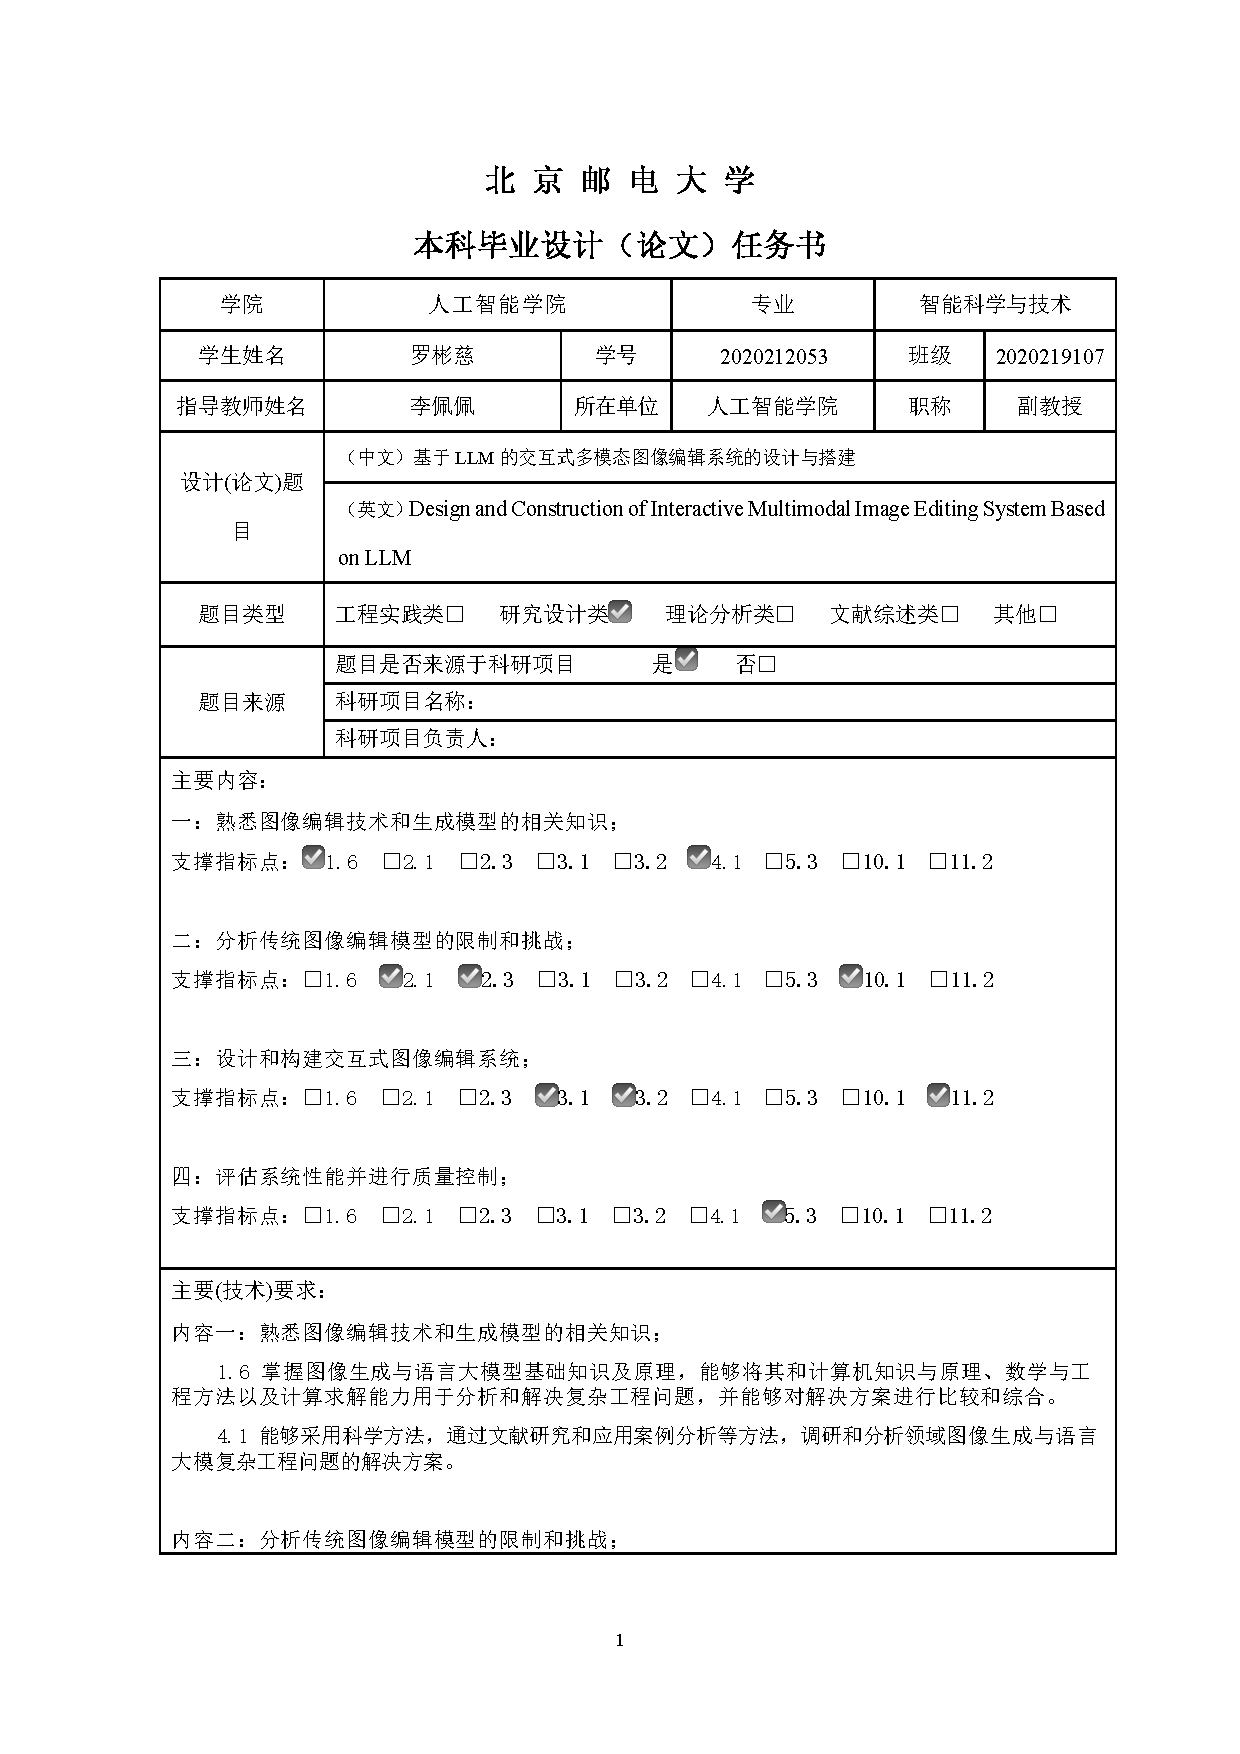
\includepdf[pages=-]{docs/task.pdf}  

% 开题报告
\blankmatter
\phantomsection\addcontentsline{toc}{chapter}{开\quad{}题\quad{}报\quad{}告}
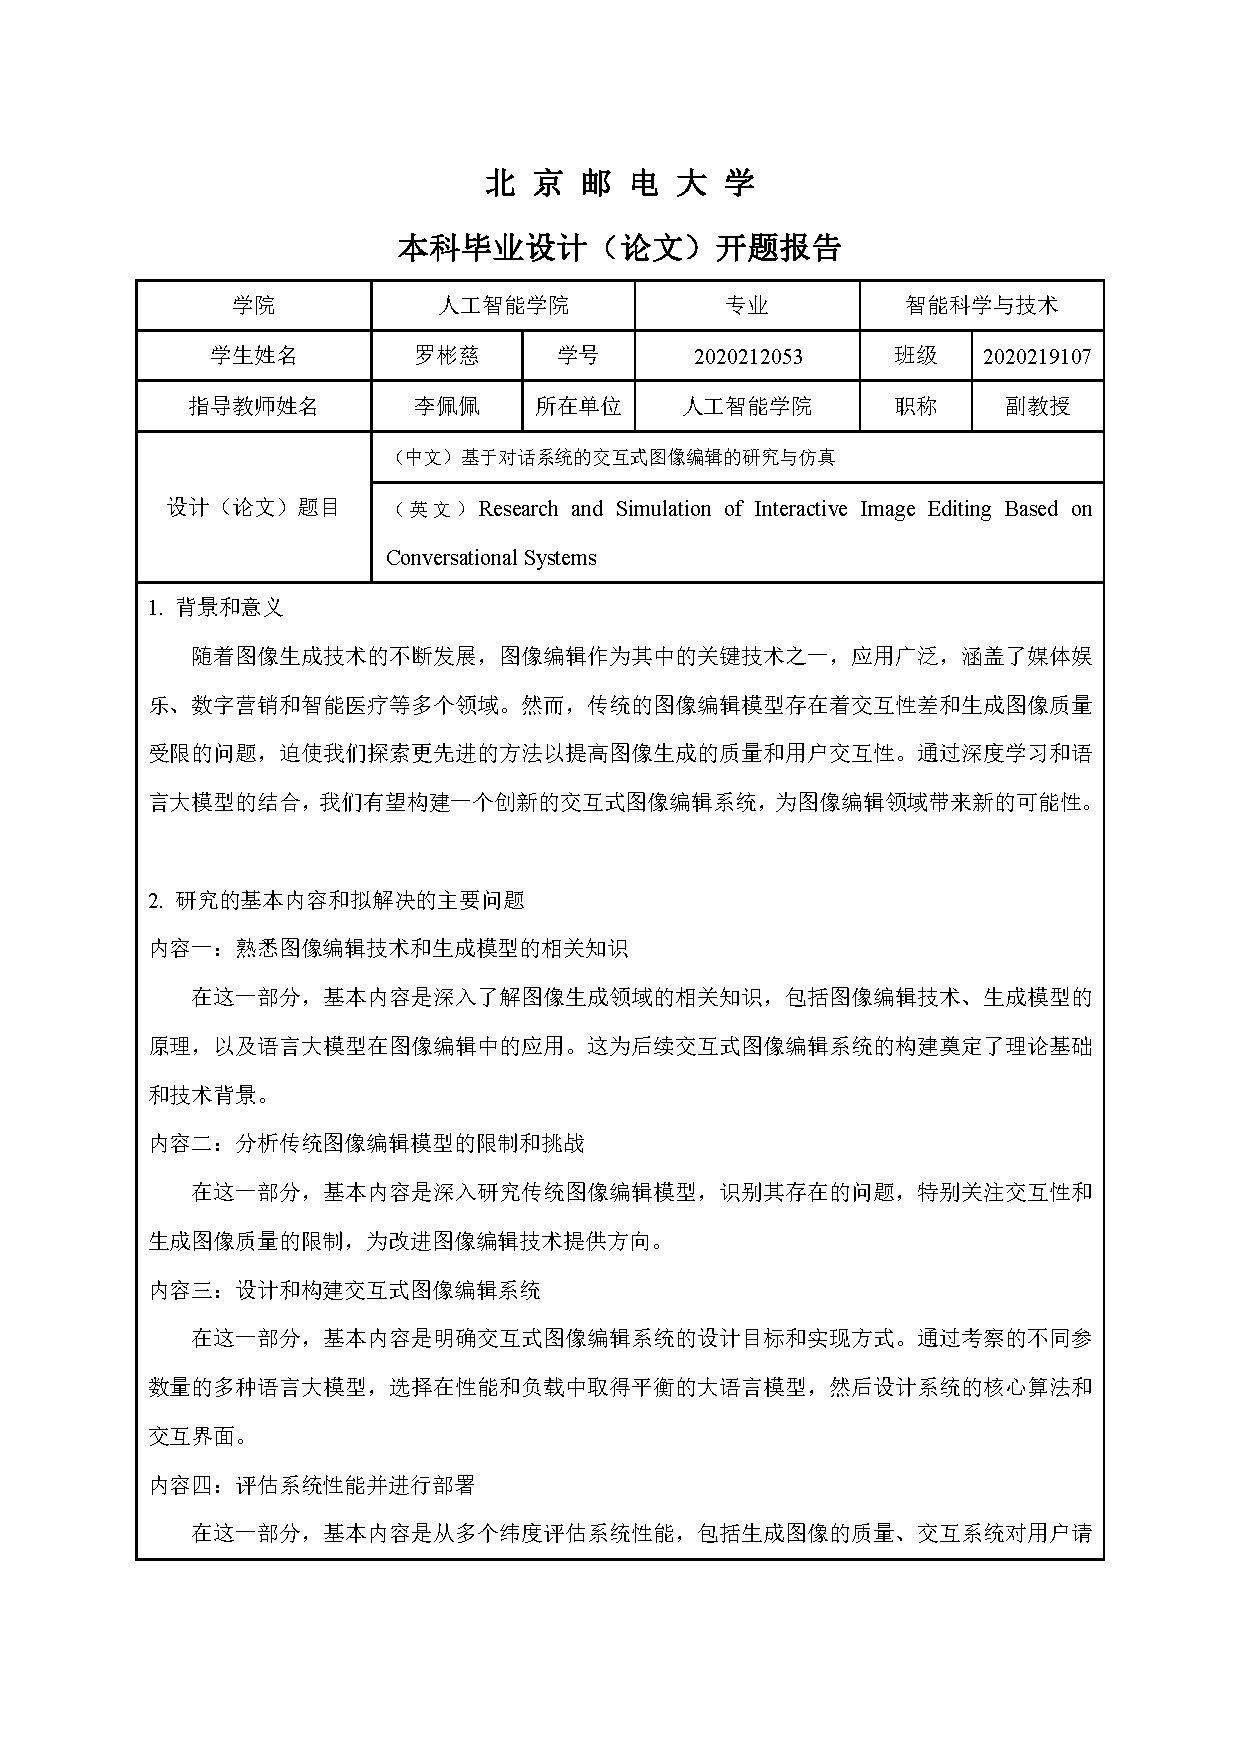
\includepdf[pages=-]{docs/openingReport.pdf}

% 中期检查表
\blankmatter
\phantomsection\addcontentsline{toc}{chapter}{中\quad{}期\quad{}检\quad{}查\quad{}表}
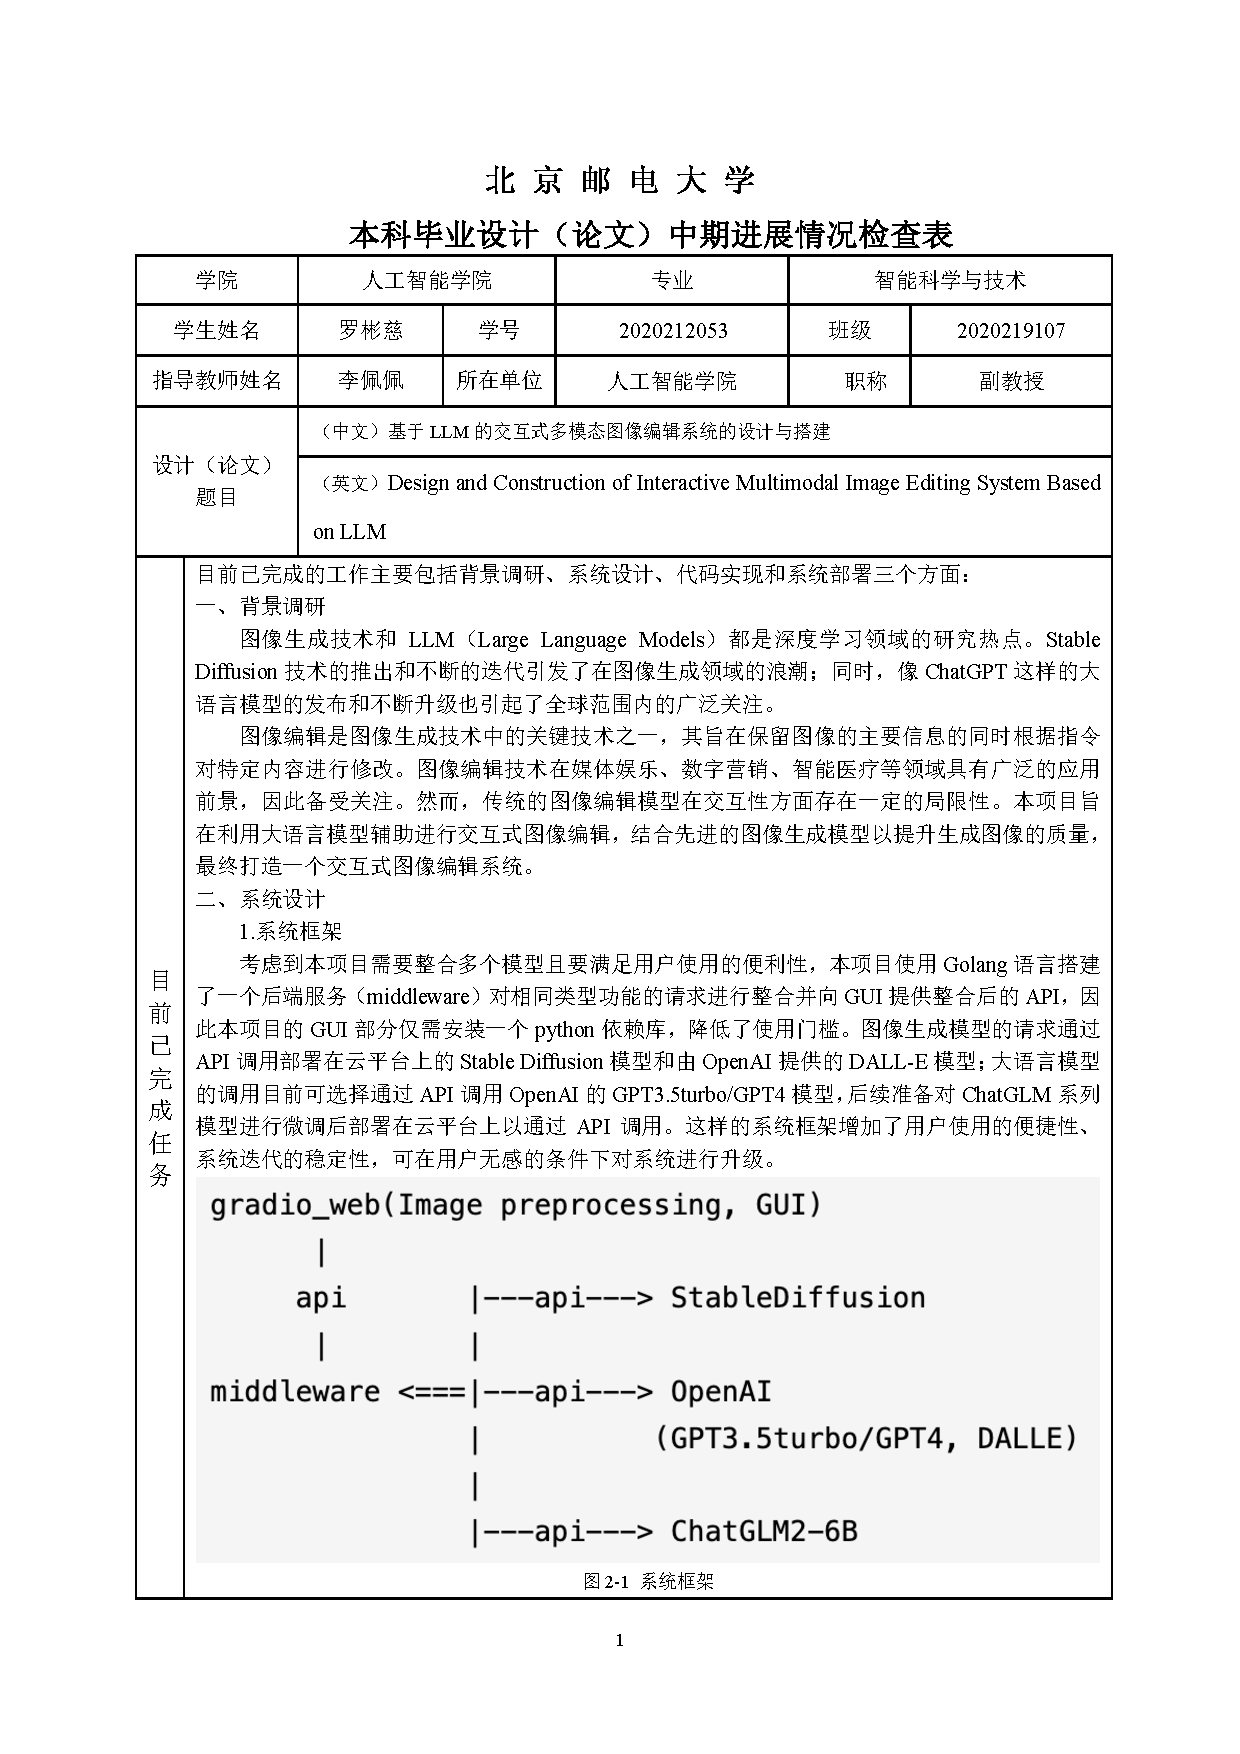
\includepdf[pages=-]{docs/interimReport.pdf}

% 教师指导毕业设计(论文)记录表
\blankmatter
\phantomsection\addcontentsline{toc}{chapter}{教师指导毕业设计(论文)记录表}
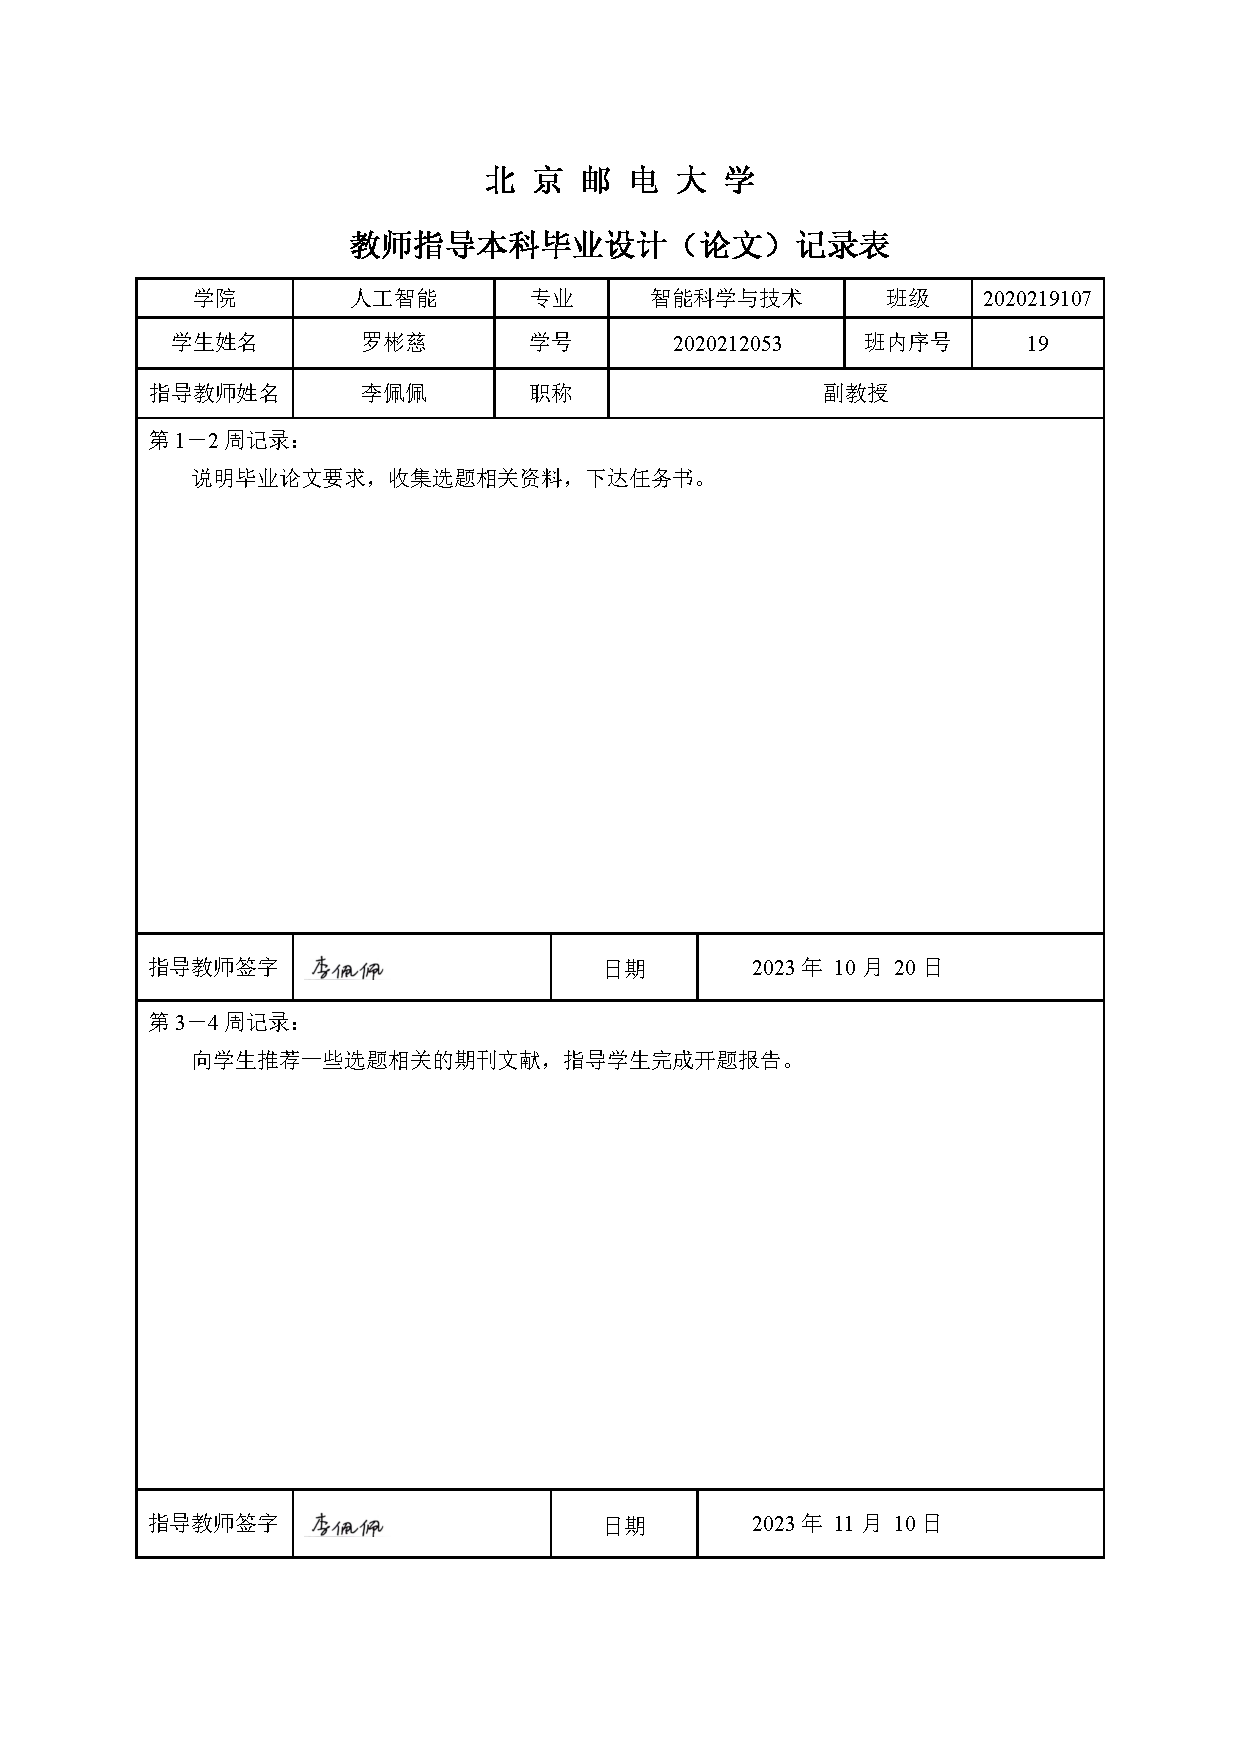
\includepdf[pages=-]{docs/guidance.pdf}

\end{nopagenumber}

\end{document}
